%% Enunturi Fizica Moleculara si Termodinamica %%

\section*{2. FIZICĂ MOLECULARĂ ŞI TERMODINAMICĂ*}
2.1. Într-un vas se află un amestec format din $60 \mathrm{~g}$ de hidrogen, cu masa molară $\mu_{\mathrm{H}}=2 \cdot 10^{-3} \mathrm{~kg} / \mathrm{mol}$ şi $120 \mathrm{~g}$ de dioxid de carbon cu masa molară $\mu_{\mathrm{CO_{2}}}=44 \cdot 10^{-3} \mathrm{~kg} / \mathrm{mol}$. Masa unui mol al acestui amestec este:\\ A) $5 \cdot 10^{-3} \mathrm{~kg} / \mathrm{mol}$; B) $5,5 \cdot 10^{-3} \mathrm{~kg} / \mathrm{mol}$; C) $6 \cdot 10^{-2} \mathrm{~kg} / \mathrm{mol}$; D) $5,5 \cdot 10^{-3} \mathrm{~kg} / \mathrm{kmol}$; E) $5 \cdot 10^{-4} \mathrm{~kg} / \mathrm{mol}$; F) $5,5 \mathrm{~kg}$.\\ (Ion M. Popescu)\\

2.2. Un motor ideal, ce funcționează după un ciclu Carnot, absoarbe într-un ciclu căldura $Q_{1}=2500 \mathrm{~J}$ de la sursa caldă. Temperatura sursei calde este $t_{1}=227^{\circ} \mathrm{C}$, iar temperatura sursei reci $t_{2}=27^{\circ} \mathrm{C}$. Căldura cedată sursei reci este:\\ A) $1500 \mathrm{~J}$; B) $1600 \mathrm{~J}$; C) $1550 \mathrm{~J}$; D) $1000 \mathrm{~J}$; E) $40 \mathrm{~J}$; F) $1605 \mathrm{~J}$.\\ (Ion M. Popescu)\\

2.3. Într-un vas de volum $V=0,3 \mathrm{~m}^{3}$ la presiunea $p_{1}=2 \cdot 10^{5} \mathrm{~N} / \mathrm{m}^{2}$ se află aer care este răcit izocor, pierzând prin răcire căldura $Q=75 \mathrm{~kJ}$. Căldura molară izocoră a aerului fiind $C_{V}=5 R / 2$, presiunea finală a acestuia este:\\ A) $10^{6} \mathrm{~N} / \mathrm{m}^{2}$; В) $5 \cdot 10^{6} \mathrm{~N} / \mathrm{m}^{2}$; C) $10^{8} \mathrm{~N} / \mathrm{m}^{2}$; D) $3 \cdot 10^{6} \mathrm{~N} / \mathrm{m}^{2}$; E) $10^{5} \mathrm{~N} / \mathrm{m}^{2}$; F) $5 \cdot 10^{5} \mathrm{~N} / \mathrm{m}^{2}$.\\ (Ion M. Popescu)\\

2.4. $200 \mathrm{~g}$ de azot se încălzesc la presiune constantă de la temperatura de $20^{\circ} \mathrm{C}$ la $100{ }^{\circ} \mathrm{C}$, căldura specifică a azotului la presiune constantă fiind $c_{p}=1040 \mathrm{~J} / \mathrm{kg} \cdot \mathrm{K}$. Cantitatea de căldură necesară pentru efectuarea acestui proces este:\\ A) $10 \mathrm{~kJ}$; B) $14 \mathrm{~kJ}$; C) $16,64 \mathrm{~kJ}$; D) $14,64 \mathrm{~kJ}$; E) $13,36 \mathrm{~kJ}$; F) $5 \mathrm{~kJ}$.\\ (Ion M. Popescu)\\

2.5. Un gaz care se găseşte într-o stare inițială (1) caracterizată prin parametrii $p_{1}=5 \cdot 10^{5} \mathrm{~N} / \mathrm{m}^{2}$ şi $V_{1}=3 \cdot 10^{-3} \mathrm{~m}^{3}$ poate ajunge în starea (2), situată pe aceeaşi izotermă şi caracterizată prin $p_{2}=3,75 \cdot 10^{5} \mathrm{~N} / \mathrm{m}^{2}$ printr-o transformare izocoră, urmatǎ de una izobară ($1 \rightarrow 3 \rightarrow 2$) (Fig. 2.1). Lucrul mecanic efectuat pentru acest proces este:\\ A) $300 \mathrm{~J}$; B) $350 \mathrm{~J}$; C) $400 \mathrm{~J}$; D) $375 \mathrm{~J}$; E) $380 \mathrm{~J}$; F) $100 \mathrm{~J}$.\\ (Ion M. Popescu)\\ 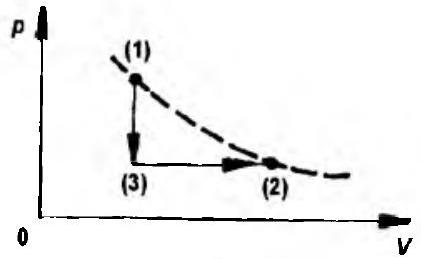
\includegraphics[max width=\textwidth, center]{2025_07_01_5b3ff9fa0d508c8e9f17g-074} Fig. 2.1\\

2.6. O masă de oxigen de volum $V_{1}=2 \mathrm{~m}^{3}$ se află la presiunea $p_{1}=2 \cdot 10^{5} \mathrm{~N} / \mathrm{m}^{2}$. Gazul are $C_{V}=5 R / 2$. El este încălzit izobar şi se destinde până la volumul $V_{2}=6 \mathrm{~m}^{3}$, apoi izocor până ce presiunea devine $p_{3}=5 \cdot 10^{5} \mathrm{~N} / \mathrm{m}^{2}$. Variația energiei interne în aceste procese este:\\ A) $6 \cdot 10^{6} \mathrm{~J}$; B) $6,4 \cdot 10^{6} \mathrm{~J}$; C) $6,5 \cdot 10^{5} \mathrm{~J}$; D) $3 \cdot 10^{8} \mathrm{~J}$; E) $10^{7} \mathrm{~J}$; F) $6,5 \cdot 10^{6} \mathrm{~J}$.\\ (Ion M. Popescu)\\

2.7.* Încălzind un gaz cu $\Delta T=100 \mathrm{~K}$, viteza termică a moleculelor creşte de la $v_{T_{1}}=400 \mathrm{~m} / \mathrm{s}$ la $v_{T_{2}}=500 \mathrm{~m} / \mathrm{s}$. Constanta generală a gazelor fiind $R=8,31 \mathrm{~J} / \mathrm{mol} \cdot \mathrm{K}$ gazul are masa molară:\\ A) $29 \mathrm{~kg} / \mathrm{kmol}$; B) $28 \cdot 10^{-3} \mathrm{~kg} / \mathrm{mol}$; C) $32 \cdot 10^{-3} \mathrm{~kg} / \mathrm{mol}$; D) $30 \mathrm{~kg} / \mathrm{kmol}$; E) $28 \mathrm{~kg} / \mathrm{mol}$; F) $14 \cdot 10^{-3} \mathrm{~kg} / \mathrm{mol}$.\\ (Ion M. Popescu)\\

2.8. În condiții normale de temperatură şi presiune ($T=273,15 \mathrm{~K}$ şi $p=1 \mathrm{~atm}$), numărul lui Avogadro find $N_{A}=6,0234 \cdot 10^{23} \mathrm{molecule} / \mathrm{mol}$ şi volumul molar $V_{\mu_{0}}=22,42 \cdot 10^{-3} \mathrm{~m}^{3} / \mathrm{mol}$, numărul de molecule aflate într-un volum $V=1 \mathrm{~m}^{3}$ de oxigen sau de azot este:\\ A) $2,7 \cdot 10^{25}$ molecule, $2,5 \cdot 10^{25}$ molecule; B) $2 \cdot 10^{26}$ molecule; C) $2,5 \cdot 10^{25}$ molecule, $2,8 \cdot 10^{25}$ molecule; D) $2,7 \cdot 10^{25}$ molecule; E) $2 \cdot 10^{26}$ molecule, $3 \cdot 10^{25}$ molecule; F) $8 \cdot 10^{32}$ molecule.\\ (Ion M. Popescu)\\

2.9. Numărul lui Avogadro fiind $N_{A}=6,024 \cdot 10^{23}$ molecule $/ \mathrm{mol}$ şi masa moleculară a oxigenului $\mu_{\mathrm{O}_{2}}=32 \cdot 10^{-3} \mathrm{~kg} / \mathrm{mol}$ într-o masă de $2 \mathrm{~kg}$ de oxigen se găseşte un număr de molecule egal cu:\\ A) $3,765 \cdot 10^{25}$ molecule; B) $3 \cdot 10^{25}$ molecule; C) $3 \cdot 10^{26}$ molecule; D) $3,765 \cdot 10^{26}$ molecule; E) $2,765 \cdot 10^{25}$ molecule; F) $3,8 \cdot 10^{25}$ molecule.\\ (Ion M. Popescu)\\

2.10.* Numărul lui Avogadro este $N_{A}=6,023 \cdot 10^{23}$ molecule $/ \mathrm{mol}$. Presiunea azotului find $p=56 \cdot 10^{3} \mathrm{Nm}^{2}$, viteza termică $v_{T}=600 \mathrm{~m} / \mathrm{s}$ şi masa moleculară $\mu=28 \cdot 10^{-3} \mathrm{~kg} / \mathrm{mol}$, concentrația moleculelor acestuia este:\\ A) $10^{24} \mathrm{~m}^{-3}$; B) $5 \cdot 10^{24} \mathrm{~m}^{-3}$; C) $10^{25} \mathrm{~m}^{-3}$; D) $3 \cdot 10^{25} \mathrm{~m}^{-3}$; E) $5 \cdot 10^{32} \mathrm{~m}^{-3}$; F) $2 \cdot 10^{25} \mathrm{~m}^{-3}$.\\ (Ion M. Popescu)\\

2.11. Dacă un agregat pentru obținerea vidului ar permite realizarea unei presiuni într-un vas egală cu $p=10^{-13} \mathrm{~torr}$, numărul moleculelor de gaz aflate într-un volum $V=1 \mathrm{~cm}^{3}$ la presiunea amintită şi temperatura $T=360 \mathrm{~K}$ ($N_{A}=6,023 \cdot 10^{23}$ molecule $/ \mathrm{mol}$ şi $R=8,31 \mathrm{~J} / \mathrm{mol} \cdot \mathrm{K}$) ar fi:\\ A) $2,68 \cdot 10^{4}$ molecule; B) $3 \cdot 10^{4}$ molecule; C) $3,5 \cdot 10^{3}$ molecule; D) $4 \cdot 10^{4}$ molecule; E) $5,3 \cdot 10^{3}$ molecule; F) $2,68 \cdot 10^{3}$ molecule.\\ (Ion M. Popescu)\\

2.12. Într-o butelie de volum $V=6,25 \mathrm{~m}^{3}$, se păstrează oxigen comprimat la presiunea $p=100 \mathrm{~atm}$ şi temperatura $t=27^{\circ} \mathrm{C}$. În condiții normale de temperatură şi presiune ($T_{0}=273 \mathrm{~K}$ şi $p_{0}=1 \mathrm{~atm}$), volumul oxigenului este:\\ A) $560 \mathrm{~m}^{3}$; B) $565 \mathrm{~m}^{3}$; C) $467,25 \mathrm{~m}^{3}$; D) $570 \mathrm{~m}^{3}$; E) $568,75 \mathrm{~m}^{3}$; F) $568 \mathrm{~m}^{3}$.\\ (Ion M. Popescu)\\

2.13. Dioxidul de carbon ($\mu=44 \cdot 10^{-3} \mathrm{~kg} / \mathrm{mol}$), aflat într-un volum $V=50$ litri la temperatura $t=2^{\circ} \mathrm{C}$ şi presiunea $p=1,66 \cdot 10^{7} \mathrm{~N} / \mathrm{m}^{2}$ are masa ($R=8,31 \mathrm{~J} / \mathrm{mol} \cdot \mathrm{K}$):\\ A) $16 \mathrm{~kg}$; B) $13 \mathrm{~kg}$; C) $15 \mathrm{~kg}$; D) $15,5 \mathrm{~kg}$; E) $17 \mathrm{~kg}$; F) $14 \mathrm{~kg}$.\\ (Ion M. Popescu)\\

2.14. Un gaz aflat în condiţii normale de temperatură și presiune ($T_{0}$ şi $p_{0}$) are densitatea $\rho_{0}$, iar când se schimbă condițiile de temperatură şi presiune devenind $T \neq T_{0}$ şi $p \neq p_{0}$, densitatea gazului este:\\ A) $\frac{p}{p_{0}} \frac{T}{T_{0}} \frac{1}{\rho_{0}}$; B) $\frac{p_{0}}{p} \frac{T_{0}}{T} \rho_{0}$; C) $p p_{0} \frac{T}{T_{0}} \rho_{0}$; D) $p p_{0} T T_{0} \rho_{0}$; E) $\frac{p p_{0}}{T T_{0} \rho_{0}}$; F) $\rho_{0} \frac{p}{p_{0}} \frac{T_{0}}{T}$.\\ (Ion M. Popescu)\\

2.15. Într-un cilindru cu piston se află aer la presiunea atmosferică normală $p_{0}=10^{5} \mathrm{~N} / \mathrm{m}^{2}$, pistonul având masa neglijabilă şi secţiunea $S=250 \mathrm{~cm}^{2}$. Inițial, pistonul se află la distanța $d_{1}=1,8 \mathrm{~m}$ de fundul cilindrului și pentru a-1 aduce încet la distanța $d_{2}=1,2 \mathrm{~m}$ se acționează asupra pistonului pentru a ajunge în poziția finală (frecările fiind neglijabile) cu forța:\\ A) $1 \mathrm{~kN}$; B) $1,25 \mathrm{~kN}$; C) $1,5 \mathrm{~kN}$; D) $2 \mathrm{~kN}$; E) $1,3 \mathrm{~kN}$; F) $8 \mathrm{~kN}$.\\ (Ion M. Popescu)\\

2.16. Într-un vas de volum $V=0,2075 \mathrm{~m}^{3}$ se află heliu (de masă molară $\mu=4 \cdot 10^{-3} \mathrm{~kg} / \mathrm{mol}$) la presiunea $p_{1}=1,2 \cdot 10^{5} \mathrm{~N} / \mathrm{m}^{2}$ şi temperatura $t_{1}=27^{\circ} \mathrm{C}$. Introducând heliu în vas până când presiunea a devenit $p_{2}=2,8 \cdot 10^{5} \mathrm{~N} / \mathrm{m}^{2}$ şi temperatura $t_{2}=47^{\circ} \mathrm{C}$, masa heliului introdus este ($R=8,3 \mathrm{IJ} / \mathrm{mol} \cdot \mathrm{K}$):\\ A) $4,5 \cdot 10^{-2} \mathrm{~kg}$; B) $4,75 \cdot 10^{-2} \mathrm{~kg}$; C) $4,75 \cdot 10^{-3} \mathrm{~kg}$; D) $4,55 \cdot 10^{-2} \mathrm{~kg}$; E) $4 \cdot 10^{-2} \mathrm{~kg}$; F) $5 \cdot 10^{-2} \mathrm{~kg}$.\\ (Ion M. Popescu)\\

2.17. Un vas cilindric orizontal conține un gaz împărțit cu ajutorul unui perete mobil în două părţi, având raportul volumelor $V_{1} / V_{2}=0,8$. Temperatura gazului de volum $V_{1}$ este $t_{1}=167^{\circ} \mathrm{C}$, iar temperatura gazului de volum $V_{2}$ este $t_{2}=255^{\circ} \mathrm{C}$. Presiunea în ambele compartimente este aceeaşi, egalǎ cu $p$. Când cele două parți ale vasului sunt aduse la aceeaşi temperatură, raportul volumelor ocupate de cele două gaze devine:\\ A) $0,9$; B) $0,94$; C) $0,98$; D) $1,2$; E) $0,96$; F) $0,38$.\\ (Ion M. Popescu)\\

2.18. În condiții normale de temperatură şi presiune ($T_{0}=273 \mathrm{~K}$, $p=101325 \mathrm{~N} / \mathrm{m}^{2}$) densitatea gazului este $\rho_{0}=1,293 \mathrm{~kg} / \mathrm{m}^{3}$ şi coeficientul adiabatic $\gamma=1,41$, adică gazul are căldura specifică la presiune constantă $c_{p}$:\\ A) $900 \mathrm{~J} / \mathrm{kgK}$; B) $980 \mathrm{~J} / \mathrm{kgK}$; C) $800 \mathrm{~J} / \mathrm{kgK}$; D) $987 \mathrm{~J} / \mathrm{kgK}$; E) $1000 \mathrm{~J} / \mathrm{kgK}$; F) $500 \mathrm{~J} / \mathrm{kgK}$.\\ (Ion M. Popescu)\\

2.19. Se cunosc $N_{A}=6,023 \cdot 10^{23}$ molecule $/ \mathrm{mol}$ şi $k_{B}=1,38 \cdot 10^{-23} \mathrm{~J} \cdot \mathrm{~K}^{-1}$. Un gaz cu căldură specificã izobară $c_{p}=5,2 \cdot 10^{3} \mathrm{~J} / \mathrm{kg} \cdot \mathrm{K}$ şi căldura specifică izocoră $c_{v}=3,2 \cdot 10^{3} \mathrm{~J} / \mathrm{kg} \cdot \mathrm{K}$, are masa molară:\\ A) $4 \cdot 10^{-3} \mathrm{~kg} \cdot \mathrm{~mol}^{-1}$; B) $4,14 \cdot 10^{-3} \mathrm{~kg} \cdot \mathrm{~mol}^{-1}$; C) $3,92 \cdot 10^{-3} \mathrm{~kg} \cdot \mathrm{~mol}^{-1}$; D) $4,2 \cdot 10^{-3} \mathrm{~kg} \cdot \mathrm{~mol}^{-1}$; E) $5 \cdot 10^{-3} \mathrm{~kg} \cdot \mathrm{~mol}^{-1}$; F) $4,3 \cdot 10^{-3} \mathrm{~kg} \cdot \mathrm{~mol}^{-1}$.\\ (Ion M. Popescu)\\

2.20. O cantitate de oxigen ($C_{V}=5 R / 2$) ocupă volumul $V_{1}=1,2 \mathrm{~m}^{3}$ la presiunea $p_{1}=2,5 \cdot 10^{5} \mathrm{~N} / \mathrm{m}^{2}$. Gazul este încălzit izobar şi se destinde până la volumul $V_{2}=3,2 \mathrm{~m}^{3}$, apoi izocor până la presiunea $p_{3}=5,25 \cdot 10^{5} \mathrm{~N} / \mathrm{m}^{2}$ şi în aceste procese variația energiei interne a gazului este:\\ A) $3,45 \mathrm{~MJ}$; B) $3 \mathrm{~MJ}$; C) $10 \mathrm{~kJ}$; D) $3,45 \mathrm{~kJ}$; E) $3,5 \mathrm{~MJ}$; F) $3,8 \mathrm{~kJ}$.\\ (Ion M. Popescu)\\

2.21. Un gaz care participă la o transformare ciclică al cărei randament este $\eta=0,1$, efectuează lucrul mecanic $L=400 \mathrm{~J}$. În decursul acestui ciclu, căldura cedată de gaz la sursa rece este:\\ A) $3000 \mathrm{~J}$; B) $4000 \mathrm{~J}$; C) $-3600 \mathrm{~J}$; D) $5000 \mathrm{~J}$; E) $6000 \mathrm{~J}$; F) $-2000 \mathrm{~J}$.\\ (Ion M. Popescu)\\

2.22. Un gaz se află în condiții normale de temperatură şi presiune dacă:\\ A) $t=0^{\circ} \mathrm{C}$ şi $p=1\mathrm{~atm}$; B) $t=20^{\circ} \mathrm{C}$ şi $p=1 \mathrm{~atm}$; C) $t=0^{\circ} \mathrm{C}$ şi $p=10^{6} \mathrm{~N} / \mathrm{m}^{2}$; D) $t=273^{\circ} \mathrm{C}$ şi $p=10^{5} \mathrm{~N} / \mathrm{m}^{2}$; E) $T=0 \mathrm{~K}$ şi $p=1 \mathrm{~atm}$; F) $T=0 \mathrm{~K}$ şi $p=1,013 \cdot 10^{5} \mathrm{~N} / \mathrm{m}^{2}$.\\ (Ion M. Popescu)\\

2.23. Numărul de molecule dintr-un mol de substanță este:\\ A) $6,023 \cdot 10^{26}$; B) $6,023 \cdot 10^{23}$; C) $6,023 \cdot 10^{-26}$; D) $6,023 \cdot 10^{-23}$; E) $6,023 \cdot 10^{25}$; F) $6,023 \cdot 10^{22}$.\\ (Alexandru M. Preda)\\

2.24. Legea formulată astfel "volume egale de gaze diferite, aflate în aceleaşi condiții de temperatură și presiune, au acelaşi număr de molecule", reprezintă:\\ A) Legea lui Dalton; B) Legea proporțiilor definite; C) Legea lui Brown; D) Legea lui Avogadro; E) Legea proporțiilor multiple; F) Legea volumelor a lui Gay-Lussac.\\ (Alexandru M. Preda)\\

2.25. Un mol de substanţă se defineşte astfel:\\ A) cantitatea de substanță a cărei densitate este numeric egală cu masa moleculară a substanței date; B) cantitatea de substanță a cărei masă molară este egală cu a 12-a parte din masa atomică a izotopului de carbon $\left({ }_{6}^{12} \mathrm{C}\right)$; C) cantitatea de substanță a cărei masă, exprimată în grame, este numeric egală cu masa moleculară relativă a substanței date; D) cantitatea de substanță a cărei masă exprimată în kilograme este numeric egală cu masa moleculară a substanței date; E) cantitatea de substanță care conține $6,023 \cdot 10^{26}$ molecule; F) cantitatea de substanță aflată în condiții normale de temperatură şi presiune.\\ (Alexandru M. Preda)\\

2.26. Să se calculeze numărul de molecule dintr-un kilogram de apă dacă masa moleculară relativă a apei este $\mu=18$ şi numărul lui Avogadro este $N_{A}=$ $=6,023 \cdot 10^{23} \mathrm{molecule} / \mathrm{mol}$:\\ A) $10^{20}$; B) $3 \cdot 10^{26}$; C) $3 \cdot 10^{20}$; D) $3,301 \cdot 10^{21}$; E) $3,346 \cdot 10^{25}$; F) $10^{23}$.\\ (Alexandru M. Preda)\\

2.27. Energia internă a gazului ideal este o funcție de forma:\\ A) $U=U(t, p)$; B) $U=U(p / V)$; C) $U=U_{0}=$ const; D) $U=U(p, T)$; E) $U=U(V, T)$; F) $U=U(T)$.\\ (Alexandru M. Preda)\\

2.28. Pentru un mol de gaz ideal monoatomic energia internă va fi:\\ A) $U=\frac{2}{3} R T$; B) $U=\frac{3}{2} R T$; C) $U=\frac{3}{2} k T$; D) $U=\frac{3 R}{\mu} T$; E) $U=\frac{5}{2} R T$; F) $U=k n T$.\\ (Alexandru M. Preda)\\

2.29. Într-un tub de televizor se gǎsesc urme de aer care la temperatura de $320 \mathrm{~K}$ are o presiune de $10^{-4} \mathrm{~N} / \mathrm{m}^{2}$. Constanta lui Boltzmann $k=1,38 \cdot 10^{-23} \mathrm{~J} / \mathrm{K}$. Concentrația moleculelor din tubul de televizor este:\\ A) $0,44 \mathrm{~m}^{-3}$; B) $1,38 \cdot 10^{-21} \mathrm{~m}^{-3}$; C) $2,26 \cdot 10^{16} \mathrm{~m}^{-3}$; D) $10^{23} \mathrm{~m}^{-3}$; E) $6,023 \cdot 10^{23} \mathrm{~m}^{-3}$; F) $4,46 \cdot 10^{9} \mathrm{~m}^{-3}$.\\ (Alexandru M. Preda)\\

2.30. Un mol de gaz ideal aflat în condiţii normale de temperatură şi presiune ocupă un volum de $22,42 \mathrm{~m}^{3} / \mathrm{kmol}$. Care este valoarea constantei universale a gazelor, exprimată în $\mathrm{J} / \mathrm{mol} \cdot \mathrm{K}$?\\ A) $8,31 \cdot 10^{3}$; B) $0,0831$; C) $8,22$; D) $8,31$; E) $831,4$; F) $8341$.\\ (Alexandru M. Preda)\\

2.31. Capacitatea calorică şi căldura specifică ale unui corp solid sunt date de expresiile:\\ A) $C=\frac{U-p V}{m \Delta T}, c=\frac{Q}{\Delta T}$; B) $C=Q \Delta T, c=m Q \Delta T$; C) $C=\frac{v Q}{\Delta T}, c=\frac{v Q}{m \Delta T}$; D) $C=\frac{p V}{\Delta T}, c=\frac{Q}{\Delta T}$; Е) $C=\frac{U}{\Delta T}, c=\frac{v U}{m \Delta T}$; F) $C=\frac{Q}{\Delta T}, c=\frac{Q}{m \Delta T}$.\\ (Alexandru M. Preda)\\

2.32. Să se afle căldurile molare $C_{V}$ şi $C_{p}$ ale unui gaz perfect dacă $\gamma=1,41$ şi $R=8,31 \mathrm{~J} / \mathrm{mol} \cdot \mathrm{K}$.\\ A) $32,58 \mathrm{~J} / \mathrm{mol} \cdot \mathrm{K} 40,89 \mathrm{~J} / \mathrm{mol} \cdot \mathrm{K}$; B) $10,27 \mathrm{~J} / \mathrm{mol} \cdot \mathrm{K} \quad 18,58 \mathrm{~J} / \mathrm{mol} \cdot \mathrm{K}$; C) $20,27 \mathrm{~J} / \mathrm{mol} \cdot \mathrm{K} \quad 28,58 \mathrm{~J} / \mathrm{mol} \cdot \mathrm{K}$; D) $8,31 \mathrm{~J} / \mathrm{mol} \cdot \mathrm{K} \quad 16,62 \mathrm{~J} / \mathrm{mol} \cdot \mathrm{K}$; E) $70,10 \mathrm{~J} / \mathrm{mol} \cdot \mathrm{K} \quad 78,41 \mathrm{~J} / \mathrm{mol} \cdot \mathrm{K}$; F) $22,42 \mathrm{~J} / \mathrm{mol} \cdot \mathrm{K} \quad 8,14 \mathrm{~J} / \mathrm{mol} \cdot \mathrm{K}$.\\ (Alexandru M. Preda)\\

2.33. Lucrul mecanic efectuat de un mol de gaz ideal într-o transformare izotermă de la starea inițială $\left(V_{1}, p_{1}\right)$ la starea finală $\left(V_{2}, p_{2}\right)$ este dat de expresia:\\ A) $L=\left(V_{2}-V_{1}\right)\left(p_{2}-p_{1}\right)$; B) $L=0$; C) $L=C_{p}\left(V_{2}-V_{1}\right)$; D) $L=2,3 R T \lg \frac{p_{2}}{p_{1}}$; E) $L=2,3 R T \lg \frac{V_{2}}{V_{1}}$; F) $L=R T \ln \frac{V_{2} p_{2}}{V_{1} p_{1}}$.\\ (Alexandru M. Preda)\\

2.34. Să se calculeze cantitatea de căldură absorbită de o cantitate de apă cu masa $m=2 \mathrm{~kg}$ pentru a trece de la temperatura $t_{1}=20^{\circ} \mathrm{C}$ la $t_{2}=80^{\circ} \mathrm{C}$. Se dã: $c=4200 \mathrm{~J} / \mathrm{kg} \cdot \mathrm{K}$.\\ A) $504 \mathrm{~kJ}$; B) $504 \mathrm{~J}$; C) $120 \mathrm{~J}$; D) $252 \mathrm{~kJ}$; E) $8400 \mathrm{~J}$; F) $672 \mathrm{~kJ}$.\\ (Alexandru M. Preda)\\

2.35. Ce căldură se degajă la răcirea cu $10^{\circ} \mathrm{C}$ a unui calorifer cu masa de $10 \mathrm{~kg}$ şi căldura specifică $500 \mathrm{~J} / \mathrm{kg} \cdot \mathrm{K}$?\\ A) $5000 \mathrm{~J}$; B) $5 \cdot 10^{-3} \mathrm{~J}$; C) $5 \mathrm{~J}$; D) $5 \cdot 10^{4} \mathrm{~J}$; E) $500 \mathrm{~J}$; F) $10^{4} \mathrm{~J}$.\\ (Alexandru M. Preda)\\

2.36. Să se afle densitatea aerului dintr-o cameră în care presiunea $p=1 \mathrm{~atm}$ şi temperatura $t=27^{\circ} \mathrm{C}$. Se consideră: masa molară a aerului $\mu=29 \cdot 10^{-3} \mathrm{~kg} / \mathrm{mol}$ şi $R=8,31 \mathrm{~J} / \mathrm{K} \cdot \mathrm{mol}$.\\ A) $10 \mathrm{~kg} / \mathrm{m}^{3}$; B) $1001,18 \mathrm{~kg} / \mathrm{m}^{3}$; C) $1,18 \mathrm{~kg} / \mathrm{m}^{3}$; D) $0,01 \mathrm{~kg} / \mathrm{m}^{3}$; E) $1,1 \cdot 10^{-3} \mathrm{~kg} / \mathrm{m}^{3}$; F) $29 \mathrm{~kg} / \mathrm{m}^{3}$.\\ (Alexandru M. Preda)\\

2.37. Un gaz aflat inițial la temperatura de $0^{\circ} \mathrm{C}$ este încălzit sub presiune constantă până când volumul său se dublează. La ce temperatură a ajuns gazul în urma acestui proces?\\ A) $100^{\circ} \mathrm{C}$; B) $273^{\circ} \mathrm{C}$; C) $273 \mathrm{~K}$; D) $2730 \mathrm{~K}$; E) $819 \mathrm{~K}$; F) $5460 \mathrm{~K}$.\\ (Alexandru M. Preda)\\

2.38. Prin sistemul de răcire al unui compresor se scurge într-o oră un volum de $1,8 \mathrm{~m}^{3}$ de apă care se încălzeşte în compresor cu $6^{\circ} \mathrm{C}$. Care este puterea consumată de motor şi utilizată pentru funcționarea compresorului dacă randamentul acestuia din urmă este $60 \%$? Se consideră: căldura specifică a apei $c=4200 \mathrm{~J} / \mathrm{kgK}$ şi densitatea apei $\rho=1000 \mathrm{~kg} / \mathrm{m}^{3}$.\\ A) $45,2 \mathrm{~kW}$; B) $100 \mathrm{~kW}$; C) $25,5 \mathrm{~kW}$; D) $10,5 \mathrm{~kW}$; E) $31,5 \mathrm{~kW}$; F) $40 \mathrm{~kW}$.\\ (Alexandru M. Preda)\\

2.39. Un motor termic funcţionează după ciclul Otto format din două izocore $2-3$ şi $4-1$ şi două adiabate $1-2$ şi $3-4$. Să se afle randamentul motorului dacă $\varepsilon^{\gamma-1}=3$, unde $\varepsilon$ este raportul de compresie $V_{1} / V_{2}$ al substanței de lucru, $\gamma$ iar este exponentul adiabatic.\\ A) $0,33$; B) $0,66$; C) $0,50$; D) $0,25$; E) $0,55$; F) $0,77$.\\ (Alexandru M. Preda)\\

2.40. Ciclul Diesel reprezentat în Fig. 2.2 are ca substanțã de lucru un gaz pentru care $\gamma=C_{p} / C_{V}=1,40$. $1-2$ şi $3-4$ transformări adiabate. Dacă se consideră raportul de compresie adiabaticá $n=V_{1} / V_{2}=10$ şi raportul de destindere preliminară $k=V_{3} / V_{2}=2$, să se afle randamentul ciclului,, ştiind că $2^{1,4}=2,64$ şi $10^{0,4}=2,51$.\\ A) $0,64$; B) $0,46$; C) $0,33$; D) $0,54$; E) $0,73$; F) $0,40$.\\ (Alexandru M. Preda)\\ 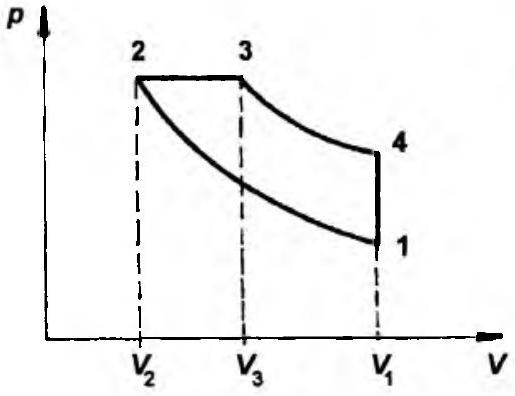
\includegraphics[max width=\textwidth, center]{2025_07_01_5b3ff9fa0d508c8e9f17g-081} Fig. 2.2\\

2.41. Un gaz ideal se află la temperatura de $300 \mathrm{~K}$ şi are energia cinetică medie a tuturor particulelor sale egală cu $6,2 \mathrm{~J}$. Dacă constanta lui Boltzmann $\k=1,38 \cdot 10^{-23} \mathrm{~J} / \mathrm{K}$ să se afle numărul total de particule care formează acest gaz ideal.\\ A) $10^{21}$; B) $10^{23}$; C) $5 \cdot 10^{20}$; D) $6 \cdot 10^{23}$; E) $10^{26}$; F) $10^{18}$.\\ (Alexandru M. Preda)\\

2.42. O maşină termică funcționează cu  $\nu \mathrm{~moli}$ de gaz perfect după ciclul din Fig. 2.3. Transformările $2-3$ şi $4-1$ sunt izoterme cu temperaturile $T_{2}=500 \mathrm{~K}$ şi respectiv $T_{1}=300 \mathrm{~K}$. Dacă transformările rectilinii $1-2$ şi $3-4$ au căldurile molare egale cu $2 R$ şi unghiul $\alpha=30^{\circ}$, să se afle randamentul ciclului. Se consideră: $\ln 3=1$.\\ A) $0,30$; B) $0,15$; C) $0,66$; D) $0,33$; E) $0,50$; F) $0,20$.\\ (Alexandru M. Preda)\\ 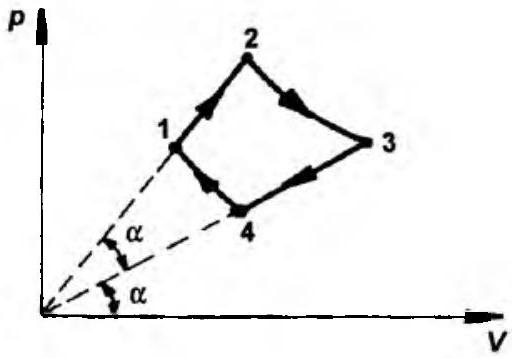
\includegraphics[max width=\textwidth, center]{2025_07_01_5b3ff9fa0d508c8e9f17g-081(1)} Fig. 2.3\\

2.43. Într-un cilindru orizontal închis la un capăt se află un piston mobil și o rezistență $R_{1}$, de volum neglijabil, conectată la o sursă exterioară de tensiune $U=10 \mathrm{~V}$ şi rezistență internă neglijabilă (Fig. 2.4). În compartimentul închis de lungime $L$ în poziția inițială de echilibru la temperatura $T_{0}=300 \mathrm{~K}$ se află $\nu=4 / R$ moli de gaz perfect monoatomic. Să se determine valoarea rezistenței $R_{1}$ astfel ca după timpul $\tau=60 \mathrm{~s}$ de la conectarea sursei la rezistența $R_{1}$ noua poziție de echilibru a pistonului mobil să fie la $L_{1}=1,25 L$. Se presupune că întreaga căldură degajată de rezistența $R_{1}$ este absorbitã de gazul din compartimentul închis.\\ A) $4 \Omega$; B) $40 \Omega$; C) $0,25 \Omega$; D) $8 \Omega$; E) $25 \Omega$; F) $100 \Omega$.\\ (Alexandru M. Preda)\\ 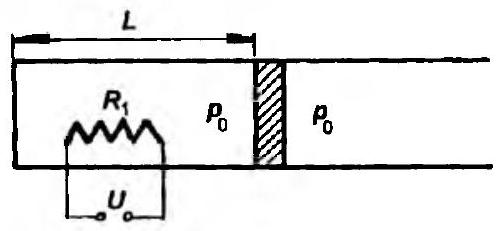
\includegraphics[max width=\textwidth, center]{2025_07_01_5b3ff9fa0d508c8e9f17g-082} Fig. 2.4\\

2.44. Sub acțiunea unei forțe orizontale un corp care are căldura specifică $c=100 \mathrm{~J} / \mathrm{kg} \cdot \mathrm{grad}$ se deplasează uniform pe un plan orizontal având coeficientul de frecare $\mu=0,5$. Dacă se presupune că numai jumătate din căldura degajată prin frecare este absorbită de corp să se afle cu cât creşte temperatura lui după ce a parcurs distanța $s=80 \mathrm{~m}$ ($g=10 \mathrm{~m} / \mathrm{s}^{2}$).\\ A) 4 grade; B) 0,4 grade; C) 1 grad; D) 2 grade; E) 0,5 grade; F) 8 grade.\\ (Alexandru M. Preda)\\

2.45. Un gaz ideal al cărui exponent adiabatic este $\gamma$ suferă o dilatare descrisă de ecuația $p=b V$ unde $b>0$ este o constantă. În cursul dilatării presiunea creşte de la $p_{1}$ la $p_{2}=n p_{1}$. Variația energiei interne a gazului în acest proces este:\\ A) $(\gamma+1) b n V_{1}^{2}$; B) $(\gamma-1) n^{2} b V_{1}^{2}$; C) $\frac{n^{2} b V_{1}^{2}}{\gamma-1}$; D) $\frac{\left(n^{2}-1\right) b V_{1}^{2}}{\gamma-1}$; E) $\gamma b\left(n^{2}-1\right) V_{1}^{2}$; F) $\frac{\left(n^{2}+1\right) b V_{1}^{2}}{\gamma+1}$.\\ (Constantin P. Cristescu)\\

2.46. Raportul dintre presiunea şi densitatea unui gaz ideal este constant în transformarea:\\ A) izobară; B) în orice transformare; C) izotermă; D) în nici o transformare; E) adiabaticǎ; F) izocoră.\\ (Constantin P. Cristescu)\\

2.47. Într-un calorimetru cu capacitate calorică neglijabilă se amestecă mase egale din acelaşi lichid aflate la temperaturile $t_{1}=30^{\circ} \mathrm{C}, t_{2}=6^{\circ} \mathrm{C}$ şi $t_{3}=87^{\circ} \mathrm{C}$. Temperatura amestecului este:\\ A) $32^{\circ} \mathrm{C}$; B) $55^{\circ} \mathrm{C}$; C) $35^{\circ} \mathrm{C}$; D) $47^{\circ} \mathrm{C}$; E) $38^{\circ} \mathrm{C}$; F) $41^{\circ} \mathrm{C}$.\\ (Constantin P. Cristescu)\\

2.48. Un mol de gaz ideal aflat la temperatura $t_{1}=37^{\circ} \mathrm{C}$ suferă o transformare izobară în care efectuează lucrul mecanic $L=1662 \mathrm{~J}$. Cunoscând $R=8,31 \mathrm{~J} / \mathrm{mol} \cdot \mathrm{K}$ temperatura gazului în starea finală este:\\ A) $510 \mathrm{~K}$; B) $470 \mathrm{~K}$; C) $544 \mathrm{~K}$; D) $483 \mathrm{~K}$; E) $220^{\circ} \mathrm{C}$; F) $183^{\circ} \mathrm{C}$.\\ (Constantin P. Cristescu)\\

2.49. O maşină termică ideală funcționează după un ciclu Carnot între temperaturile $t_{1}=227^{\circ} \mathrm{C}$ şi $t_{2}=27^{\circ} \mathrm{C}$ producând în cursul unui ciclu un lucru mecanic $L=8 \cdot 10^{4} \mathrm{~J}$. Căldura cedată sursei reci într-un ciclu este:\\ A) $3 \cdot 10^{5} \mathrm{~J}$; B) $1,2 \cdot 10^{5} \mathrm{~J}$; C) $1,8 \cdot 10^{5} \mathrm{~J}$; D) $3,6 \cdot 10^{5} \mathrm{~J}$; E) $2,8 \cdot 10^{5} \mathrm{~J}$; F) $4,2 \cdot 10^{5} \mathrm{~J}$.\\ (Constantin P. Cristescu)\\

2.50.* Un gaz ideal suferă o transformare generală în care presiunea se dublează iar densitatea se înjumătățeşte. Viteza termică a moleculelor se modifică astfel:\\ A) se înjumătățeşte; B) se dublează; C) creşte de $\sqrt{2}$ ori; D) scade de $\sqrt{2}$ ori; E) scade de $4$ ori; F) rămâne nemodificată.\\ (Constantin P. Cristescu)\\

2.51.* Într-o incintǎ se află oxigen ( $\mu=32 \cdot 10^{-3} \mathrm{~kg} / \mathrm{mol}$ ) la presiunea $p=8 \cdot 10^{4} \mathrm{~N} / \mathrm{m}^{2}$, viteza termică a moleculelor find $v_{T}=500 \mathrm{~m} / \mathrm{s}$.

Considerând numǎrul lui Avogadro $N_{A}=6 \cdot 10^{23} \mathrm{molec} / \mathrm{mol}$ concentrația $n$ a moleculelor din vas este:\\
A) $10^{24} \mathrm{molec} / \mathrm{m}^{3}$;\\
B) $2,5 \cdot 10^{24} \mathrm{molec} / \mathrm{m}^{3}$;\\
C) $2,7 \cdot 10^{25} \mathrm{molec} / \mathrm{m}^{3}$;\\
D) $3 \cdot 10^{25} \mathrm{molec} / \mathrm{m}^{3}$;\\
E) $1,8 \cdot 10^{25} \mathrm{molec} / \mathrm{m}^{3}$;\\
F) $5,3 \cdot 10^{24} \mathrm{molec} / \mathrm{m}^{3}$.\\
(Constantin P. Cristescu)\\
2.52. Randamentul unei maşini termice care ar funcționa după un ciclu Carnot între două surse ale căror temperaturi coincid cu temperaturile maximă şi minimă atinse în ciclul desenat în Fig. 2.5 este:\\
A) $\frac{1}{3}$;\\
B) $\frac{2}{3}$;\\
C) $\frac{5}{6}$,\\
D) $\frac{1}{6}$;\\
E) $\frac{4}{5}$;\\
F) nu poate fi calculat din datele furnizate.\\
(Constantin P. Cristescu)\\
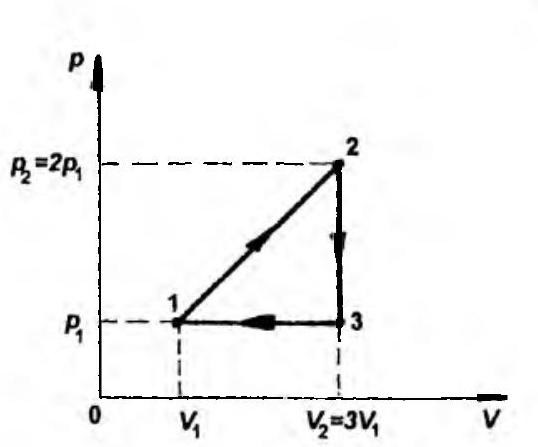
\includegraphics[max width=\textwidth, center]{2025_07_01_5b3ff9fa0d508c8e9f17g-084}\\
2.53. Un gaz ideal monoatomic având volumul $V_{1}$ la presiunea $p_{1}$ este comprimat izobar până la volumul $V_{2}=\frac{V_{1}}{n}$ şi apoi încălzit izocor până la presiunea $p_{2}=\frac{n}{2} p_{1}$. Dacă în starea inițială energia internă este $U_{1}$, energia $U_{2}$ în starea finală este:\\
A) $2 U_{1}$;\\
B) $U_{1}$;\\
C) $\left(\frac{n}{2}+1\right) U_{1}$;\\
D) $\frac{n}{2} U_{1}$;\\
E) $\frac{2 U_{1}}{n}$;\\
F) $\frac{U_{1}}{2}$.\\
2.54. Se consideră transformările unei mase de gaz ideal reprezentate grafic în Zégura 2.6. Dacă între pantele lor există relația $\operatorname{tg} \alpha_{1}=\frac{1}{2} \operatorname{tg} \alpha_{2}=\frac{1}{3} \operatorname{tg} \alpha_{3}$ care s.ntre următoarele afirmații este eronată ?\\
A) transformările sunt izobare; B) $p_{2}=\frac{p_{1}+p_{3}}{2}$;\\
C) pentru curba 3 presiunea este cea mai mică;\\
D) pentru curba 1 presiunea este cea mai mare;\\
E) $p_{2}=\frac{p_{1}}{2}$; F) $\frac{p_{3}}{p_{2}}=\frac{2}{3}$.\\
(Constantin P. Cristescu)\\
2.55. Un tub de lungime $L$ închis la un capăt se scufundǎ vertical cu capătul Leschis în jos intr-un lichid cu densitatea $\rho=10^{3} \mathrm{~kg} / \mathrm{m}^{3}$, porțiunea scufundată suand lungimea $l=66 \mathrm{~cm}$. Lungimea coloanei de lichid din tub este $l^{\prime}=6 \mathrm{~cm}$. Considerând $g=10 \mathrm{~m} / \mathrm{s}^{2}$ şi ştiind că presiunea atmosferică $p_{0}=10^{5} \mathrm{~N} / \mathrm{m}^{2}$, -ngimea $L$ a tubului este:\\
A) 106 cm ;\\
B) 100 cm ;\\
C) $98,8 \mathrm{~cm}$;\\
D) 95 cm ;\\
E) 110 cm ;\\
F) 101 cm .\\
(Constantin P. Cristescu)\\
2.56. Deschizând un vas, presiunea gazului scade cu $f_{1}=28 \%$, iar :emperatura absolută cu $f_{2}=10 \%$. Cu cât la sută scade masa gazului ?\\
A) $33,3 \%$;\\
B) $30 \%$;\\
C) $20 \%$;\\
D) $25 \%$;\\
E) $21 \%$;\\
F) $40 \%$.\\
2.57. Randamentul ciclului din Fig. 2.7 este (se cunoaşte coeficientul adiabatic $\because$ al gazului care execută ciclul):\\
A) $\eta=\frac{\gamma-1}{\gamma+1}$;\\
B) $\eta=\frac{3}{2} \frac{\gamma-1}{6 \gamma+1}$;\\
C) $\eta=\frac{\gamma-1}{6 \gamma-1}$;\\
D) $\eta=\frac{2(\gamma-1)}{\gamma+1}$;\\
Е) $\eta=\frac{3(\gamma-1)}{6 \gamma+1}$;\\
F) $\eta=\frac{3 \gamma}{6 \gamma+1}$.\\
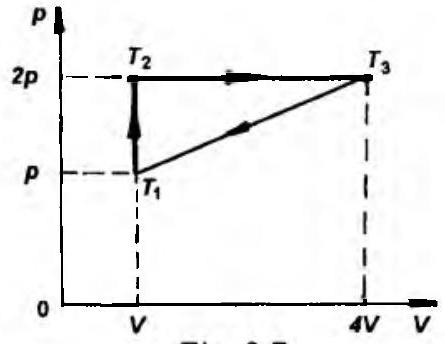
\includegraphics[max width=\textwidth, center]{2025_07_01_5b3ff9fa0d508c8e9f17g-085}

Fig. 2.7\\
2.58. Un vas cilindric cu secțiunea de $10 \mathrm{~cm}^{2}$ şi masa de 200 g , aşezat pe un plan orizontal cu gura în jos, închide aer la temperatura de $27^{\circ} \mathrm{C}$ şi presiunea atmosferică normală de $10^{5} \mathrm{~N} / \mathrm{m}^{2}$. Găsiți concentrația moleculelor din vasul cilindric şi temperatura la care aerul începe să iasă din vas. Se cunoaşte $k=1,38 \cdot 10^{-23} \mathrm{~J} / \mathrm{K}$.\\
A) $n=24 \cdot 10^{25} \mathrm{~m}^{-3} ; T_{2}=35^{\circ} \mathrm{C}$;\\
B) $n=12 \cdot 10^{24} \mathrm{~m}^{-3} ; T_{2}=300 \mathrm{~K}$;\\
C) $n=2,4 \cdot 10^{25} \mathrm{~m}^{-3} ; T_{2}=306 \mathrm{~K}$;\\
D) $n=2,4 \cdot 10^{25} \mathrm{~m}^{-3} ; T_{2}=275 \mathrm{~K}$;\\
E) $n=20 \cdot 10^{24} \mathrm{~m}^{-3} ; T_{2}=288 \mathrm{~K}$;\\
F) $n=2,4 \cdot 10^{25} \mathrm{~m}^{-3} ; T_{2}=316 \mathrm{~K}$.

\section*{(Maria Honciuc)}
2.59. Un motor termic funcționează după un ciclu Carnot cu randamentul de $40 \%$. Temperatura sursei reci este de $27^{\circ} \mathrm{C}$, iar maşina primeşte de la sursa caldă cantitatea de căldură de 60 kJ în fiecare secundă. Să se găsească cu câte grade ar trebui coborâtă temperatura sursei reci astfel încât randamentul motorului să crească la $50 \%$ şi care este puterea inițială a motorului:\\
A) $50^{\circ} \mathrm{C} ; 2,4 \mathrm{~kW}$; B) 50 K ; 24 kW ; C) $20^{\circ} \mathrm{C} ; 12 \mathrm{~kW}$;\\
D) 20 K ; 24 kW ; E) 50 K ; 25 kW ; F) 50 K ; 60 kW .\\
(Maria Honciuc)\\
2.60. Un gaz ideal diatomic disociază în proporție de $f$ procente din moleculele sale. Căldura molară izocoră a gazului format este:\\
(Se cunosc $C_{V_{1}}=\frac{3}{2} R ; C_{V_{2}}=\frac{5}{2} R ; f=0,5$ ).\\
A) $C=\frac{5}{6} R$;\\
B) $C=\frac{15}{6} R$;\\
C) $C=\frac{6}{11} R$;\\
D) $C=\frac{11}{6} R$;\\
E) $C=\frac{5}{2} R$;\\
F) $C=2 R$.\\
2.61. Formula fundamentală a teoriei cinetico-moleculare este:\\
A) $p=\frac{2}{3} N \frac{\bar{v}^{2}}{2}$;\\
B) $p=\frac{1}{3} N m \bar{v}^{2}$;\\
C) $p=\frac{2}{3} \frac{N}{V} \frac{m \bar{v}^{2}}{2}$;\\
D) $p=N k T$;\\
E) $p=\frac{2}{3} N \bar{\varepsilon}$;\\
F) $p=\frac{2}{3} N \frac{m \bar{v}^{2}}{3}$.\\
2.62.* Un gaz ideal $(\gamma=7 / 5)$ se destinde adiabatic de la $V_{1}$ la $V_{2}=32 V_{1}$. Raportul vitezelor termice ale moleculelor este:\\
A) $3 / 2$;\\
B) 4 ;\\
C) 2,4 ;\\
D) 0,5 ;\\
E) 2 F) 4,2 .\\
(Corneliu Ghizdeanu)\\
2.63. Căldura schimbatã în procesul $1-2$ din F.g. 2.8 este:\\
А) 0 ; В) $n p_{0} V_{0} \ln (1 / n)$;\\
C) $(1 / 2) p_{0} V_{0}\left(n^{2}-1\right)$;\\
D) $n p_{0} V_{0} \ln (n)$;\\
Е) $\frac{p_{0} V_{0}}{2}\left(1-n^{2}\right)$;\\
F) $\frac{p_{0} V_{0}}{2}\left(1-2 n^{2}\right)$.\\
(Corneliu Ghizdeanu)\\
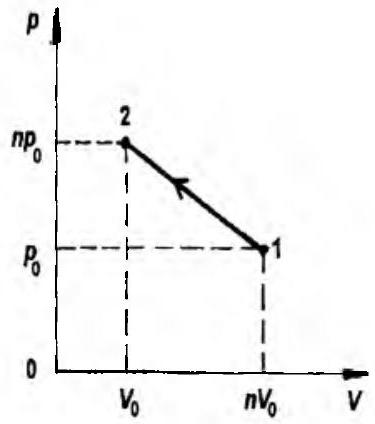
\includegraphics[max width=\textwidth, center]{2025_07_01_5b3ff9fa0d508c8e9f17g-087}

Fig. 2.8\\
2.64.* Viteza termică a unei mici picături de ază $r$ şi de densitate $\rho$ aflată în aer la temperatura $T$ este:\\
A) $\frac{3}{2} \sqrt{k T /\left(\pi \rho r^{3}\right)}$;\\
В) $\frac{3}{2} \sqrt{k} \bar{T} / \pi \rho r^{3}$;\\
C) $\frac{1}{2} \sqrt{k T /\left(\pi \rho r^{3}\right)}$;\\
D) $\sqrt{3 k T / \mu}$;\\
E) $\sqrt{3 R T / m}$;\\
F) $\frac{3}{2} \sqrt{k T /\left(\pi \rho^{2} r^{3}\right)}$.\\
(Corneliu Ghizdeanu)\\
2.65.* Două vase $V_{1}$ şi $V_{2}$ legate printr-un tub de volum neglijabil conțin același gaz la presiunea $p$ şi temperatura $T_{1}$. Vasul $V_{1}$ se încălzeşte la $o$ :emperatură $T_{1}^{\prime}=n T_{1}$, iar vasul $V_{2}$ rămâne la temperatura $T_{1}$. Variația relativă a itezei termice a moleculelor din vasul $V_{1}$ este:\\
A) $\sqrt{n}$;\\
B) $1-\sqrt{n}$;\\
C) $\sqrt{n}-1$;\\
D) $\frac{\sqrt{n}}{n}$;\\
E) $n^{2}$;\\
F) $-\frac{\sqrt{n}}{n}$.\\
(Corneliu Ghizdeanu)\\
2.66. O masă de gaz se află închisă într-un vas la presiunea $p_{0}$ şi volumul $V_{0}$. Dacã presiunea gazului este schimbată izoterm cu $2 \cdot 10^{5} \mathrm{~N} / \mathrm{m}^{2}$ volumul acestuia se schimbă cu $3 \cdot 10^{-3} \mathrm{~m}^{3}$, iar la o schimbare izotermă cu $5 \cdot 10^{5} \mathrm{~N} / \mathrm{m}^{2}$ a presiunii, volumul se modifică cu $5 \cdot 10^{-3} \mathrm{~m}^{3}$. Care sunt valorile inițiale ale presiunii şi volumului gazului ?\\
A) $p_{0}=10^{5} \frac{\mathrm{~N}}{\mathrm{~m}^{2}} ; V_{0}=5 \cdot 10^{-3} \mathrm{~m}^{3} ;$ B) $p_{0}=4 \cdot 10^{5} \frac{\mathrm{~N}}{\mathrm{~m}^{2}} ; V_{0}=9 \cdot 10^{-3} \mathrm{~m}^{3}$;\\
C) $p_{0}=9 \cdot 10^{5} \frac{\mathrm{~N}}{\mathrm{~m}^{2}} ; V_{0}=10^{-2} \mathrm{~m}^{3} ;$ D) $p_{0}=10^{5} \frac{\mathrm{~N}}{\mathrm{~m}^{2}} ; V_{0}=10^{-2} \mathrm{~m}^{3} ;$\\
E) $p_{0}=3 \cdot 10^{5} \frac{\mathrm{~N}}{\mathrm{~m}^{2}} ; V_{0}=2 \cdot 10^{-1} \mathrm{~m}^{3} ;$ F) $p_{0}=4 \cdot 10^{4} \frac{\mathrm{~N}}{\mathrm{~m}^{2}} ; V_{0}=9 \cdot 10^{-1} \mathrm{~m}^{3}$.\\
(Marcel Dobre)\\
2.67.* Ce temperatură corespunde unei viteze termice a moleculelor de gaz egală cu viteza unui avion supersonic $v=700 \mathrm{~m} / \mathrm{s}$. Se cunosc: $\mu=29 \mathrm{~kg} / \mathrm{kmol}$, $R=8314 \mathrm{~J} / \mathrm{kmol} \cdot \mathrm{K}$.\\
A) 300 K ; B) 250 K ; C) 570 K ; D) 800 K ; E) 1000 K ; F) 750 K .\\
(Marcel Dobre)\\
2.68. Care este densitatea hidrogenului la $T=273,15 \mathrm{~K}$ şi presiunea $p=10^{5} \mathrm{~N} / \mathrm{m}^{2}$. Se cunosc $\mu=2 \mathrm{~kg} / \mathrm{kmol}, R=8314 \mathrm{~J} / \mathrm{kmol} \cdot \mathrm{K}$.\\
A) $1,293 \mathrm{~kg} / \mathrm{m}^{3}$;\\
B) $8,93 \mathrm{~kg} / \mathrm{m}^{3}$;\\
C) $0,88 \mathrm{~kg} / \mathrm{m}^{3}$;\\
D) $4 \cdot 10^{3} \mathrm{~kg} / \mathrm{m}^{3}$;\\
E) $2 \mathrm{~kg} / \mathrm{m}^{3}$;\\
F) $0,088 \mathrm{~kg} / \mathrm{m}^{3}$.\\
(Marcel Dobre)\\
2.69. Ce căldură molară izocoră are un gaz ideal care destinzându-se adiabatic îşi creşte volumul de 100 de ori şi-şi miçorează temperatura de 10 ori ? Se cunoaşte constanta gazelor ideale $R$.\\
A) $2 R$;\\
B) $3 R / 2$;\\
C) $3 R$;\\
D) $5 R$;\\
E) $R$;\\
F) $5 R / 2$.\\
(Marcel Dobre)\\
2.70. Un recipient cu volumul $V=10^{-1} \mathrm{~m}^{3}$ contine aer la presiunea $p=10^{4} \mathrm{~N} / \mathrm{m}^{2}$. Recipientul se umple cu aer până la presiunea $p_{0}=10^{5} \mathrm{~N} / \mathrm{m}^{2}$ cu ajutorul unei pompe al cărei volum de lucru este $v=3 \cdot 10^{-4} \mathrm{~m}^{3}$.

Care este numărul de curse pe care trebuie să-l facă pompa?\\
A) 1500 ;\\
B) 2500 ;\\
C) 1500 ;\\
D) 2000;\\
E) 700 ;\\
F) 300 .\\
(Marcel Dobre)\\
2.71. Un mol de gaz ideal ( $C_{V}=3 R / 2$ ) aflat inițial la temperatura $T_{1}$ efectuează o transformare descrisă de relația $T=a V^{2}$, unde $a$ este o constantă pozitivă ajungând în starea finală la un volum de 3 ori mai mare. Care este căldura\\
zbsorbită de gaz în aceastã transformare ? Se cunosc: constanta gazelor ideale $R$ şi emperatura $T_{1}$.\\
A) $8 R T_{1}$;\\
B) $10 R T_{1}$;\\
C) $20 R T_{1}$;\\
D) $16 R T_{1}$;\\
E) $12 R T_{1}$; F) $4 R T_{1}$.\\
(Marcel Dobre)\\
2.72. Căldurile specifice izocoră şi respectiv izobară ale unui gaz ideal sunt $\therefore$ și $c_{p}$. Să se determine masa molară a gazului, $\mu$. Se cunoaşte constanta zazelor ideale $R$.\\
A) $\left(c_{p}-c_{V}\right) / R$;\\
В) $\left(c_{p}-c_{V}\right) R$;\\
C) $\left(c_{p}+c_{V}\right) R$;\\
D) $R /\left(c_{p}+c_{V}\right)$;\\
Е) $R / 2\left(c_{p}+c_{V}\right)$;\\
F) $R /\left(c_{p}-c_{V}\right)$.\\
(Marcel Dobre)\\
2.73. Într-un recipient cu capacitate calorică neglijabilă se află 50 litri apă la emperatura de $65^{\circ} \mathrm{C}$. Pentru a scădea temperatura apei până la $40^{\circ} \mathrm{C}$, se adaugă apá rece, cu temperatura de $15^{\circ} \mathrm{C}$, de la un robinet cu debitul de 4 litri $/ \mathrm{min}$. Robinetul trebuie deschis timp de:\\
A) 12 min 30 s ;\\
B) $12,3 \mathrm{~min}$;\\
C) $13,2 \mathrm{~min}$;\\
D) 10 min 20 s ;\\
E) 13 min 30 s ;\\
F) 13 min .\\
(Alexandru Lupaşcu)\\

2.74. Un automobil consumă $6 litri de benzină pentru un drum de 100 km . Puterea calorică a benzinei este $q=50 \mathrm{MJ} / \mathrm{kg}$, iar densitatea ei $\rho=0,9 \mathrm{~kg} / \mathrm{dm}^{3}$. Randamentul total al motorului este de $40 \%$. Forta de tracțiune a motorului este:\\
A) 920 N ;\\
B) 108 N ;\\
C) $10^{4} \mathrm{~N}$;\\
D) 2400 N ;\\
E) 816 N ;\\
F) 1080 N .\\
(Alexandru Lupaşcu)\\

2.75. O anumită cantitate de gaz ideal ( $\gamma=1,4$ ) trece din starea inițială 1 în starea finală 2 pe două căi: mai întâi printr-o adiabată urmată de o izocoră; apoi printr-o izocoră urmată de o adiabată. Parametrii celor două stări sunt: $p_{1}=10^{5} \mathrm{~Pa}, V_{1}=5 \mathrm{~litri}$, $p_{2}=4 p_{1}, V_{2}=1,25 \mathrm{~litri}$. Notăm cu $Q_{1}$ şi cu $Q_{2}$ căldurile schimbate de gaz pe cele două căi. Căldurile $Q_{1}$ si $Q_{2}$ sunt:\\ A) $Q_{1}=-1250 \mathrm{~J}, Q_{2}=-625 \mathrm{~J}$; B) $Q_{1}=Q_{2}=625 \mathrm{~J}$; C) $Q_{1}=Q_{2}=-625 \mathrm{~J}$; D) $Q_{2}=2 Q_{1}$, fără a putea preciza valoareaș E) $Q_{1}=-1250 \mathrm{~J}, Q_{2}=625 \mathrm{~J}$; F) $Q_{1}=1250 \mathrm{~J}, Q_{2}=-625 \mathrm{~J}$.\\ (Alexandru Lupaşcu)\\

2.76. Aerul este format în principal dintr-un amestec de $\mathrm{O}_{2}$ şi $\mathrm{N}_{2}$. Se cunosc masele molare: $m_{\mathrm{O}_{2}}=32 \mathrm{~g} / \mathrm{mol}, m_{\mathrm{N}_{2}}=28 \mathrm{~g} / \mathrm{mol}$ şi constanta gazelor perfecte $R=8,3 \mathrm{~J} / \mathrm{mol} \cdot \mathrm{K}$. Vitezele medii pătratice ale celor două gaze diferă prin $\Delta v=40 \mathrm{~m} / \mathrm{s}$. Temperatura aerului este de aproximativ:\\ A) $400 \mathrm{~K}$; B) $317^{\circ} \mathrm{C}$; C) $270 \mathrm{~K}$; D) $306 \mathrm{~K}$; E) $431 \mathrm{~K}$; F) $560 \mathrm{~K}$.\\ (Alexandru Lupaşcu)\\

2.77. O eprubetă cilindrică de sticlă este umplută complet cu $78,5 \mathrm{~cm}^{3}$ de mercur. Ansamblul are temperatura de $0^{\circ} \mathrm{C}$. Ce volum de mercur se scurge din eprubetă, dacă temperatura creşte la $90^{\circ} \mathrm{C}$ ? Se cunosc: coeficientul de dilatare al sticlei $\gamma_{\mathrm{St}}=9 \cdot 10^{-6} \mathrm{~K}^{-1}$, al mercurului $\gamma_{\mathrm{Hg}}=1,8 \cdot 10^{-4} \mathrm{~K}^{-1}$.\\ A) $0,89 \mathrm{~cm}^{3}$; B) $2,56 \mathrm{~cm}^{3}$; C) $1,21 \mathrm{~cm}^{3}$; D) $0,2 \mathrm{~cm}^{3}$; E) $0,74 \mathrm{~cm}^{3}$; F) nu se scurge nici o picătură de mercur.\\ (Alexandru Lupaşcu)\\

2.78. O maşinã termică funcționează după un ciclu Carnot ideal şi are un randament de $30 \%$, luând căldură de la o sursă cu temperatura de $390 \mathrm{~K}$. Maşina va avea un randament de $40 \%$ dacă temperatura sursei calde:\\ A) creşte cu $65^{\circ} \mathrm{C}$; B) scade cu $22^{\circ} \mathrm{C}$; C) scade cu $12 \mathrm{~K}$; D) creşte cu $70 \mathrm{~K}$; E) creşte cu $20^{\circ} \mathrm{C}$; F) creşte de 1,5 ori.\\ (Alexandru Lupaşcu)\\

2.79. O cantitate de gaz ideal absoarbe o căldură de $1,4 \mathrm{~kJ}$ şi se dilată cu $25 \mathrm{~litri}$ la presiune constantă. Energia internă creşte cu $1000 \mathrm{~J}$. Presiunea gazului este:\\ A) $2,4 \cdot 10^{5} \mathrm{~Pa}$; B) $1,6 \cdot 10^{4} \mathrm{~Pa}$; C) $1,5 \cdot 10^{5} \mathrm{~Pa}$; D) $10^{4} \mathrm{~Pa}$; E) $1,2 \cdot 10^{4} \mathrm{~Pa}$; F) nu se poate calcula.\\ (Alexandru Lupaşcu)\\

2.80. Un gaz monoatomic se află într-o incintă sub presiunea unui piston de masă $M$, care se poate mişca fără frecare cu pereții incintei (Fig. 2.9). Gazul este încălzit prin intermediul unei rezistențe electrice aflată în incintă. Dacã pistonul s-a deplasat pe distanța $H$, căldura primită de gaz este:\\ A) $Q=M g H$; B) $Q=5 M g H / 2$; C) $Q=5 M g H$; D) $Q=3 M g H / 2$; E) $Q=M g H / 2$; F) $Q=0$.\\ (Gheorghe Stanciu)\\ 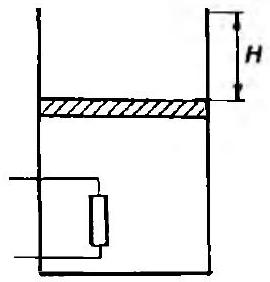
\includegraphics[max width=\textwidth, center]{2025_07_01_5b3ff9fa0d508c8e9f17g-090} Fig. 2.9\\

2.81. Într-un cilindru cu piston se află un număr $\nu$ de moli de $He$. Gazul suferă o transformare din starea 1 în starea 2 ca în Fig. 2.10. Temperatura maximă atinsă în cursul transformării 1-2 va fi:\\ A) $T_{\text {max }}=\frac{p_{1} V_{1}-p_{2} V_{2}}{v p_{1} V_{1}}$; B) $T_{\text {max }}=\frac{p_{2} V_{2}-p_{1} V_{1}}{v p_{2} V_{2}}$; C) $T_{\text {max }}=\frac{\left(p_{2} V_{1}-p_{1} V_{2}\right)^{2}}{4 v R\left(p_{2}-p_{1}\right)\left(V_{1}-V_{2}\right)}$; D) $T_{\text {max }}=\frac{\left(p_{2} V_{2}-p_{1} V_{1}\right)^{2}}{p_{2} V_{2}-p_{1} V_{1}}$; E) $T_{\text {max }}=\frac{p_{2} V_{2}}{v R}$; F) $T_{\text {max }}=\frac{\left(p_{2} V_{2}-p_{1} V_{1}\right)^{2}}{v R\left(p_{2} V_{2}-p_{1} V_{1}\right)}$.\\ (Gheorghe Stanciu)\\ 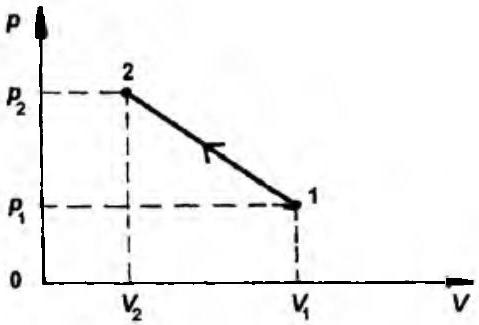
\includegraphics[max width=\textwidth, center]{2025_07_01_5b3ff9fa0d508c8e9f17g-091} Fig. 2.10\\

2.82. Un rezervor de volum $V$ este umplut cu aer la presiunea $p_{1}$ şi temperatura $T_{1}$. Rezervorul este încălzit la temperatura $T_{2},\left(T_{2}>T_{1}\right)$. Pentru ca presiunea în rezervor să rămână constantă, din rezervor este eliminată o masă $\Delta m$ de aer. Masa de aer rămasă în rezervor în funcție de $p_{1}, V, \mu, T_{1}, \Delta m$ este:\\ A) $m_{1}=\frac{p_{1} V}{\mu R T_{1}}-\Delta m$; B) $m_{1}=\frac{p_{1} V}{R T_{2}}-\Delta m$; C) $m_{1}=\frac{p_{1} T_{1}}{\mu R V}-\Delta m$; D) $m_{1}=\frac{p_{1} V}{\mu T_{2}}-R \Delta m$; E) $m_{1}=\frac{\mu p_{1} V}{R T_{1}}-\Delta m$; F) $m_{1}=\frac{\mu p_{1} V}{R T_{1}}$.\\ (Gheorghe Stanciu)\\

2.83. În figura 2.11 punctele $A$ şi $B$ se află pe aceeaşi izotermă. Să se precizeze dacă în cursul transformării de la $A$ la $B$ are loc:\\ A) o creştere a temperaturii; B) o scădere a temperaturii; C) temperatura rămâne constantă; D) o creştere a volumului şi o creştere a temperaturii; E) o creştere şi apoi o scădere a temperaturii; F) o scădere a presiunii şi o creştere a temperaturii.\\ 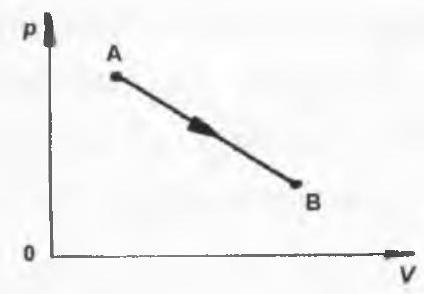
\includegraphics[max width=\textwidth, center]{2025_07_01_5b3ff9fa0d508c8e9f17g-092} Fig. 2.11\\

2.84. Un mol de gaz efectuează ciclul din Fig. 2.12. Temperaturile în punctele 1 şi 3 sunt $T_{1}$ şi respectiv $T_{3}$. Știind că punctele 2 şi 4 se află pe aceeaşi izotermă să se precizeze dacă lucrul efectuat pe ciclu este:\\ A) $R T_{1}\left(\sqrt{\frac{T_{3}}{T_{1}}}-1\right)$; B) $R T_{1} \sqrt{\frac{T_{3}}{T_{1}}}$; C) $R\left(\frac{T_{3}}{T_{1}}-1\right)$; D) $R T_{1} \sqrt{\frac{T_{1}}{T_{3}}}$; E) $R T_{1}\left(\sqrt{\frac{T_{1}}{T_{3}}}-1\right)^{2}$; F) $R T_{1}\left(\sqrt{\frac{T_{3}}{T_{1}}}-1\right)^{2}$.\\ (Gheorghe Stanciu)\\ 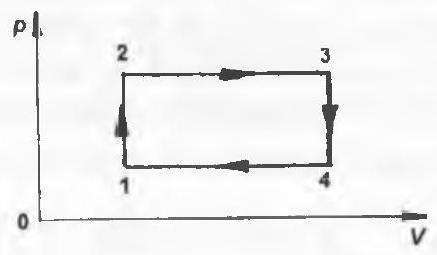
\includegraphics[max width=\textwidth, center]{2025_07_01_5b3ff9fa0d508c8e9f17g-092(1)} Fig. 2.12\\

2.85. Un mol de gaz ideal monoatomic (coeficientul adiabatic $\gamma$ ) se află inițial într-o stare caracterizată de temperatura $T_{0}$ şi presiunea $p_{0}$. Să se determine temperatura și presiunea finală a gazului în urma unei evoluții adiabatice în care are loc o triplare a volumului ocupat de gaz.\\ A) $p=\frac{p_{0}}{3^{\gamma}}, T=3^{1-\gamma} T_{0}$; B) $p=\frac{p_{0}}{3^{\gamma}}, T=3^{\gamma} T_{0}$; C) $p=\frac{p_{0}}{3^{1-\gamma}}, T=3^{\gamma} T_{0}$; D) $p=\frac{P_{0}}{3^{1-\gamma}}, T=3^{1-\gamma} T_{0}$; E) $p=\frac{2 p_{0}}{3^{\gamma}}, T=3^{1-\gamma} T_{0}$; F) $p=\frac{3 p_{0}}{3^{\gamma}}, T=3^{1-\gamma} T_{0}$.\\ (Vasile Popescu)\\

2.86. În mol de gaz ideal monoatomic (coeficientul adiabatic $\gamma$ ) se află inițial într-o stare caracterizată de temperatura $T_{0}$ şi presiunea $p_{0}$. Să se determine temperatura şi presiunea finală a gazului în urma unei evoluții izoterme în care are loc o înjumătățire a volumului ocupat de gaz.\\ A) $T=T_{0}, p=2 p_{0}$; B) $T=2 T_{0}, p=2 p_{0}$; C) $T=T_{0}, p=p_{0}$; D) $T=2 T_{0}, p=\frac{p_{0}}{2}$; E) $T=\frac{T_{0}}{2}, p=2 p_{0}$; F) $T=-\frac{T_{0}}{2}, p=\frac{p_{0}}{2}$.\\ (Vasile Popescu)\\

2.87. Un mol de gaz ideal monoatomic (coeficientul adiabatic $\gamma$ ) se află inițial intr-o stare caracterizată de presiunea $p_{0}$ şi volumul $V_{0}$. Să se determine lucrul mecanic în timpul unei evoluții adiabatice în care are loc o triplare a volumului ocupat de gaz.\\ A) $L=\frac{p_{0} V_{0}}{1-\gamma}\left(3^{1-\gamma}-1\right)$; В) $L=\frac{p_{0} V_{0}}{1-\gamma}\left(3^{1-\gamma}+1\right)$; C) $L=\frac{p_{0} V_{0}}{1-\gamma}\left(2^{1-\gamma}-1\right)$; D) $L=\frac{p_{0} V_{0}}{1+\gamma}\left(3^{1-\gamma}-1\right)$; E) $L=\frac{p_{0} V_{0}}{1+\gamma}\left(3^{1+\gamma}-1\right)$; F) $L=\frac{p_{0} V_{0}}{1-\gamma} \cdot 3^{1-\gamma}$.\\ (Vasile Popescu)\\

2.88. Un mol de gaz ideal monoatomic (coeficientul adiabatic $\gamma$ ) se află inițial intr-o stare caracterizată de presiunea $p_{0}$ şi volumul $V_{0}$. Să se determine lucrul mecanic în timpul unei evoluții izoterme în care are loc o înjumătățire a volumului ocupat de gaz.\\ A) $L=-p_{0} V_{0} \ln 2$; B) $L=-p_{0} V_{0}^{\gamma} \ln 2$; C) $L=-p_{0} V_{0}^{\gamma-1} \ln 2$; D) $L=-p_{0} V_{0} \ln 3$; E) $L=-\frac{p_{0}}{V_{0}} \ln 2$; F) $L=-\frac{p_{0} V_{0}}{\ln 2}$.\\ (Vasile Popescu)\\

2.89. Să se determine $p_{2}, T_{2}, p_{3}$ și $T_{3}$ în funcție de $p_{1}, T_{1}$ și de exponentul adiabatic $\gamma$ în cazul unui mol de gaz ideal monoatomic care este supus următoarelor transformări succesive: $\begin{aligned}& \left(p_{1}, V_{1}, T_{1}\right) \Rightarrow \frac{\text { transformare }}{\text { adiabatică }} \Rightarrow\left(p_{2}, 2 V_{1}, T_{2}\right) \Rightarrow \frac{\text { transformare }}{\text { izotermă }} \Rightarrow\left(p_{3}, V_{1}, T_{3}\right) \Rightarrow & \Rightarrow \frac{\text { transformare }}{\text { izocoră }} \Rightarrow\left(p_{1}, V_{1}, T_{1}\right) \end{aligned}$\\ A) $p_{2}=2^{-\gamma} p_{1}, T_{2}=2^{1-\gamma} T_{1}, p_{3}=\frac{p_{1}}{2^{\gamma-1}}, T_{3}=2^{1-\gamma} T_{1}$; B) $p_{2}=2^{\gamma} p_{1}, T_{2}=2^{1-\gamma} T_{1}, p_{3}=2^{\gamma} p_{1}, T_{3}=2^{\gamma} T_{1}$; C) $p_{2}=2^{-\gamma+1} p_{1}, T_{2}=2^{1-\gamma} T_{1}, p_{3}=2^{1-\gamma} p_{1}, T_{3}=2^{1-\gamma} T_{1}$; D) $p_{2}=2^{\gamma+1} p_{1}, T_{2}=2^{\gamma+1} T_{1}, p_{3}=2^{\gamma+1} p_{1}, T_{3}=2^{\gamma+1} T_{1}$; E) $p_{2}=2 p_{1}, T_{2}=2 T_{1}, p_{3}=2^{\gamma} p_{1}, T_{3}=2^{\gamma} T_{1}$; F) $p_{2}=2^{-\gamma} p_{1}, T_{2}=2^{-1-\gamma} T_{1}, p_{3}=2^{-1-\gamma} p_{1}, T_{3}=2^{-1-\gamma} T_{1}$.\\ (Vasile Popescu)\\

2.90. Să se determine lucrul mecanic total efectuat de un mol de gaz ideal monoatonic în următoarele transformări succesive: $ \left(p_{1}, V_{1}, T_{1}\right) \Rightarrow\left(p_{2}, V_{2}, T_{1}\right) \Rightarrow\left(p_{2}, V_{1}, T_{2}\right) \Rightarrow\left(p_{1}, V_{1}, T_{1}\right)$.\\ A) $p_{1} V_{1}\left(V_{2}-V_{1}\right)$; B) $p_{2}\left(V_{1}-V_{2}\right)$; C) $p_{1} V_{1} \ln \frac{V_{2}}{V_{1}}+p_{2}\left(V_{1}-V_{2}\right)$; D) $p_{1} V_{1}\left(V_{2}-V_{1}\right)+p_{2}\left(V_{1}-V_{2}\right)$; E) $p_{1} V_{1} \frac{T_{2}-T_{1}}{T_{1}}$; F) $R\left(T_{2}-T_{1}\right)$.\\ (Vasile Popescu)\\

2.91. O masă de gaz $(\mu=28 \mathrm{~kg} / \mathrm{kmol}) m=1 \mathrm{~kg}$ este încălzită cu $\Delta T=100 \mathrm{~K}$ la volum constant. Să se determine variația energiei interne. Se dau: $C_{p}=\frac{7 R}{2}$, $R=8310 \mathrm{~J} / \mathrm{kmol} \cdot \mathrm{K}$.\\ A) $74,2 \mathrm{~kJ}$; B) $7,79 \mathrm{MJ}$; C) $7,75 \mathrm{MJ}$; D) $7,4 \mathrm{~kJ}$; E) $24 \mathrm{~kJ}$; F) $27,5 \mathrm{~kJ}$.\\ (Vasile Popescu)\\

2.92. $1 \mathrm{~kmol}$ de gaz este încălzit la presiune constantă cu $10 \mathrm{~K}$. Să se determine lucrul mecanic efectuat de gaz. Se dă: $R=8310 \mathrm{~J} / \mathrm{kmol} \cdot \mathrm{K}$.\\ A) $83,1 \mathrm{~kJ}$; B) $831 \mathrm{~kJ}$; C) $31 \mathrm{~MJ}$; D) $8,31 \mathrm{~J}$; E) $8,31 \mathrm{~kJ}$; F) $31 \mathrm{~kJ}$.\\ (Vasile Popescu)\\

2.93. Să se determine căldura primită de un gaz în cazul unei transformări ciclice în care lucrul mecanic efectuat de gaz este $L=100 \mathrm{~J}$ iar randamentul ciclului este $\eta=0,2$.\\ A) $400 \mathrm{~J}$; B) $100 \mathrm{~J}$; C) $500 \mathrm{~J}$; D) $200 \mathrm{~J}$; E) $20 \mathrm{~J}$; F) $0,002 \mathrm{~J}$.\\ (Vasile Popescu)\\

2.94. Un gaz ocupă volumul $V_{1}=1 \mathrm{~litru}$ la presiunea $p_{1}=10^{5} \mathrm{~N} / \mathrm{m}^{2}$ şi temperatura $t_{1}=27^{\circ} \mathrm{C}$. Gazul este încălzit izobar până la temperatura $t_{2}=30^{\circ} \mathrm{C}$. Să se determine lucrul mecanic efectuat.\\ A) $1 \mathrm{~J}$; B) $196 \mathrm{~J}$; C) $9,6 \mathrm{~J}$; D) $2 \mathrm{~J}$; E) $1 \mathrm{~kJ}$; F) $9,6 \mathrm{~kJ}$.\\ (Vasile Popescu)\\

2.95. Un gaz ocupă volumul $V=1 \mathrm{~litru}$ la presiunea $p_{1}=10^{5} \mathrm{~N} / \mathrm{m}^{2}$. Gazul este încălzit la volum constant până când presiunea sa devine $p_{2}=2 \cdot 10^{5} \mathrm{~N} / \mathrm{m}^{2}$. Să se determine căldura $Q_{V}$ absorbită de gaz. Se dau: $C_{p}=7 R / 2, R=8310 \mathrm{~J} / \mathrm{kmol} \mathrm{K}$.\\ A) $250 \mathrm{~J}$; B) $5 \mathrm{~MJ}$; C) $250 \mathrm{~J}$; D) $500 \mathrm{~J}$; E) $250 \mathrm{~MJ}$; F) $2,5 \mathrm{~J}$.\\ (Vasile Popescu)\\

2.96. Un gaz ideal monoatomic ( $C_{V}=3 / 2 R$ ) se destinde după legea $p=a V$, unde $a=10^{8} \mathrm{~N} \cdot \mathrm{~m}^{-5}$, de la volumul $V_{1}=2 \cdot 10^{-3} \mathrm{~m}^{3}$ până la volumul $V_{2}=2 V_{1}$. Cât este căldura în această tranformare ?\\ A) $2,4 \mathrm{~kJ}$; B) $51000 \mathrm{~J}$; C) $10000 \mathrm{~J}$; D) $100 \mathrm{~J}$; E) $10 \mathrm{~kJ}$; F) $1 \mathrm{~kJ}$.\\ (Niculae N. Puşcaş)\\

2.97. În interiorul unui balon cu volumul $0,1 \mathrm{~m}^{3}$ se aflã un gaz la presiunea $2 \cdot 10^{5} \mathrm{~N} / \mathrm{m}^{2}$ şi temperatura $400 \mathrm{~K}$. Balonul este răcit până la temperatura $300 \mathrm{~K}$, presiunea gazului devenind $10^{5} \mathrm{~N} / \mathrm{m}^{2}$, iar $54,6 \mathrm{~g}$ de gaz a ieşit din balon printr-o supapă. Cât este densitatea gazului în condiții normale ? $\left(p_{0}=10^{5} \mathrm{~N} / \mathrm{m}^{2} ; T_{0}=273 \mathrm{~K}\right)$\\ A) $5 \mathrm{~kg} / \mathrm{m}^{3}$; B) $1,2 \mathrm{~kg} / \mathrm{m}^{3}$; C) $0,1 \mathrm{~kg} / \mathrm{m}^{3}$; D) $100 \mathrm{~kg} / \mathrm{m}^{3}$; E) $10,2 \mathrm{~kg} / \mathrm{m}^{3}$; F) $12 \mathrm{~kg} / \mathrm{m}^{3}$.\\ (Niculae N. Puşcaş)\\

2.98. Cât este lucrul mecanic efectuat de $\nu$ kmoli de gaz perfect când se dilată de la $T_{1}$ la $T_{2}$ ştiind că temperatura acestuia variază proporțional cu pătratul presiunii ? Se dă $R$.\\ A) $\frac{1}{2} \nu R\left(T_{2}-T_{1}\right)$; В) $\frac{5}{2} \nu R\left(T_{1}-T_{2}\right)$; C) $\frac{5}{2} \nu R\left(T_{2}-T_{1}\right)$; D) $R\left(T_{2}-T_{1}\right)$; E) $\frac{1}{2} \nu\left(T_{2}-T_{1}\right)$; F) $\frac{1}{2} \nu R\left(2 T_{2}-T_{1}\right)$.\\ (Niculae N. Puşcaş)\\

2.99. În trei vase având volumele de $3 \mathrm{~litri}$, $5 \mathrm{~litri}$ şi respectiv $2 \mathrm{~litri}$ se află trei gaze diferite la aceeaşi temperatură, presiunile corespunzătoare fiind $2 \cdot 10^{5} \mathrm{~N} / \mathrm{m}^{2}, 3 \cdot 10^{5} \mathrm{~N} / \mathrm{m}^{2}$ şi $5 \cdot 10^{5} \mathrm{~N} / \mathrm{m}^{2}$. Cât este presiunea finală a amestecului dacă cele trei vase sunt legate între ele prin tuburi de volume neglijabile?\\ A) $3,64 \mathrm{~N} / \mathrm{m}^{2}$; B) $3,1 \cdot 10^{5} \mathrm{~N} / \mathrm{m}^{2}$; C) $1,12 \mathrm{~N} / \mathrm{m}^{2}$; D) $7,41 \cdot 10^{5} \mathrm{~N} / \mathrm{m}^{2}$; E) $20 \mathrm{~N} / \mathrm{m}^{2}$; F) $4,8 \cdot 10^{5} \mathrm{~N} / \mathrm{m}^{2}$.\\ (Niculae N. Puşcaş)\\

2.100. Cât este variația energiei interne a $2 \mathrm{~g}$ de gaz ideal $\left(C_{V}=\frac{3}{2} R\right)$ pentru care în urma încălzirii viteza termică inițială de $400 \mathrm{~m} / \mathrm{s} ~ \mathrm{~s}-\mathrm{a}$ dublat ?\\ A) $100 \mathrm{~J}$; B) $10 \mathrm{~J}$; C) $2000 \mathrm{~J}$; D) $10 \mathrm{~kJ}$; E) $480 \mathrm{~J}$; F) $5000 \mathrm{~J}$.\\ (Niculae N. Puşcaş)\\

2.101. O maşină termică ideală funcționează după un ciclu Carnot, temperatura sursei reci find $300 \mathrm{~K}$, iar a celei calde cu $100 \mathrm{~K}$ mai mult. Cât este căldura cedată sursei reci ştiind că în timpul unui ciclu motorul efectuează un lucru mecanic de $0,1 \mathrm{~kJ}$ ?\\ A) $100 \mathrm{~J}$; B) $1000 \mathrm{~J}$; C) $2 \mathrm{~kJ}$; D) $300 \mathrm{~J}$; E) $5 \mathrm{~kJ}$; F) $0,9 \mathrm{~kJ}$.\\ (Niculae N. Puşcaş)\\

2.102. Două corpuri de fier $A$ şi $B$ se pun în contact termic. Corpul $A$ are masa $m_{\mathrm{A}}$ şi temperatura $t_{\mathrm{A}}=900^{\circ} \mathrm{C}$, iar corpul $B$ are masa $m_{\mathrm{B}}=2 m_{\mathrm{A}}$ şi temperatura $t_{\mathrm{B}}=t_{\mathrm{A}} / 2$. Temperatura finală de echilibru va fi:\\ A) $600^{\circ} \mathrm{C}$; B) $650^{\circ} \mathrm{C}$; C) $700^{\circ} \mathrm{C}$; D) $750^{\circ} \mathrm{C}$; E) $800^{\circ} \mathrm{C}$; F) $850^{\circ} \mathrm{C}$.\\ (Mircea Stan)\\

2.103. Un vas cilindric are un capac de greutate $5 \mathrm{~N}$ şi diametru $20 \mathrm{~cm}$. În vas se află vapori (considerați drept gaz ideal) la temperatura de $41^{\circ} \mathrm{C}$ şi presiunea de $10^{5} \mathrm{~N} / \mathrm{m}^{2}$. La ce temperatură încep vaporii să iasă afară din vas ?\\ A) $90^{\circ} \mathrm{C}$; B) $80,5^{\circ} \mathrm{C}$; C) $71,5^{\circ} \mathrm{C}$; D) $51^{\circ} \mathrm{C}$; E) $50,5^{\circ} \mathrm{C}$; F) $41,5^{\circ} \mathrm{C}$.\\ (Mircea Stan)\\

2.104. La $0^{\circ} \mathrm{C}$ densitatea uleiului este $840 \mathrm{~kg} / \mathrm{m}^{3}$. Care va fi densitatea uleiului încălzit la o temperatură la care volumul său a crescut cu $20 \%$ ?\\ A) $830 \mathrm{~kg} / \mathrm{m}^{3}$; B) $820 \mathrm{~kg} / \mathrm{m}^{3}$; C) $720 \mathrm{~kg} / \mathrm{m}^{3}$; D) $700 \mathrm{~kg} / \mathrm{m}^{3}$; E) $680 \mathrm{~kg} / \mathrm{m}^{3}$; F) $660 \mathrm{~kg} / \mathrm{m}^{3}$.\\ (Mircea Stan)\\

2.105. Care este energia cinetică medie de translație a tuturor moleculelor de aer dintr-un pahar de apă cu volumul $0,25 \mathrm{~litri}$ aflat la presiunea $p=10^{5} \mathrm{~Pa}$ ?\\ A) $2,25 \mathrm{~J}$; B) $37,5 \mathrm{~J}$; C) $18,9 \mathrm{~J}$; D) $20,25 \mathrm{~J}$; E) $21,4 \mathrm{~J}$; F) $22,38 \mathrm{~J}$.\\ (Mircea Stan)\\

2.106. Un gaz ideal monoatomic ( $C_{V}=\frac{3}{2} R$ ) primeşte căldura $Q=12,45 \mathrm{~kJ}$ pentru a-şi mări izocor temperatura $\Delta T$. Ce căldură ar fỉ necesară gazului pentru z-şi mări temperatura tot cu $\Delta T$, dar intr-o transformare izobară ?\\ A) $63,35 \mathrm{~kJ}$; B) $52,55 \mathrm{~kJ}$; C) $41,52 \mathrm{~kJ}$; D) $30,15 \mathrm{~kJ}$; E) $25,5 \mathrm{~kJ}$; F) $20,75 \mathrm{~kJ}$.\\ (Mircea Stan)\\

2.107. Ce lucru mecanic efectuează un gaz ideal în urma transformării ciclice ABC din Fig. 2.13? Se cunosc: $p_{\mathrm{A}}=p_{\mathrm{C}}=1 \mathrm{~atm} ; \quad V_{\mathrm{A}}=1,5 \mathrm{~litri}$; $V_{\mathrm{C}}=2,5 \mTHRM{~litri}$; $p_{\mathrm{B}}=3 \mathrm{~atm}$.\\ A) $1,5 \mathrm{~kJ}$; B) $100 \mathrm{~J}$; C) $3 \mathrm{~kJ}$; D) $3,5 \mathrm{~kJ}$; E) $4,5 \mathrm{~kJ}$; F) $5,5 \mathrm{~kJ}$.\\ (Mircea Stan)\\ 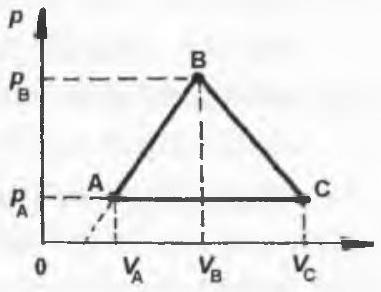
\includegraphics[max width=\textwidth, center]{2025_07_01_5b3ff9fa0d508c8e9f17g-097} Fig. 2.13\\

2.108. Randamentul unei maşini termice ideale este de $40 \%$. Cât devine randamentul dacă temperatura izvorului cald creşte de trei ori, iar temperatura izvorului rece se reduce la jumătate ?\\ A) $35 \%$; B) $48 \%$; C) $50 \%$; D) $70 \%$; E) $90 \%$; F) $95 \%$.\\ (Mircea Stan)\\

2.109. Ce lucru mecanic efectuează un gaz diatomic $\left(C_{V}=\frac{5}{2} R\right)$ care primeşte izobar căldura $Q=14,7 \mathrm{~kJ}$ ?\\ A) $4,2 \mathrm{~kJ}$; B) $6,1 \mathrm{~kJ}$; C) $8,2 \mathrm{~kJ}$; D) $9,7 \mathrm{~kJ}$; E) $10,4 \mathrm{~kJ}$; F) $11,2 \mathrm{~kJ}$.\\ (Mircea Stan)\\

2.110. Un cilindru cu sectiunea $S=3 \mathrm{~cm}^{2}$ este acoperit cu un piston de greutate neglijabilă, asupra căruia apasă forța $F=20,64 \mathrm{~N}$. În interiorul vasului se află un gaz ideal cu densitatea $\rho=1,29 \mathrm{~kg} / \mathrm{m}^{3}$. Viteza termică a moleculelor de gaz este:\\ A) $120 \mathrm{~m} / \mathrm{s}$; B) $200 \mathrm{~m} / \mathrm{s}$; C) $320 \mathrm{~m} / \mathrm{s}$; D) $400 \mathrm{~m} / \mathrm{s}$; E) $420 \mathrm{~m} / \mathrm{s}$; F) $500 \mathrm{~m} / \mathrm{s}$.\\ (Mircea Stan)\\

2.111. O moleculă de heliu ( $\mu_{\mathrm{He}}=4$ ) are masa $m=6,6 \cdot 10^{-27} \mathrm{~kg}$. Ce masă are o moleculă de magneziu ? $\left(\mu_{\mathrm{Mg}} \approx 24\right)$\\ A) $8,4 \cdot 10^{-27} \mathrm{~kg}$; B) $6,21 \cdot 10^{-26} \mathrm{~kg}$; C) $3,96 \cdot 10^{-26} \mathrm{~kg}$; D) $4,54 \cdot 10^{-27} \mathrm{~kg}$; E) $6,86 \cdot 10^{-27} \mathrm{~kg}$; F) $4,18 \cdot 10^{-26} \mathrm{~kg}$.\\ (Mircea Stan)\\

2.112. Căldura schimbată cu exteriorul de sistemele termodinamice în cursul transformărilor de stare:\\ A) este schimbată în mod izocor cu exteriorul; B) raportată la masa de substanţă transformată este egală cu o constantă de material specifică transformării considerate; C) trebuie măsurată direct, fiind imposibilă calcularea ei datorită modificării coeficienților calorici ai sistemului în cursul transformărilor de fază; D) este o măsură a energiei de agitație termică; E) se numeşte căldură latentă a transformării pentru că aceste transformări sunt, în general, transformări de durată; F) este schimbată în mod izobar cu exteriorul.\\ (Elena Slavnicu)\\

2.113. Conform Fig. 2.14, dacă presiunea $p=ct.$, ce se poate spune despre masa gazului dacă densitatea gazului rămâne constantă ?\\ A) creşte; B) depinde de presiune; C) rămâne constantă; D) depinde de pătratul presiunii; E) scade; F) creşte şi apoi scade.\\ (Elena Slavnicu)\\ 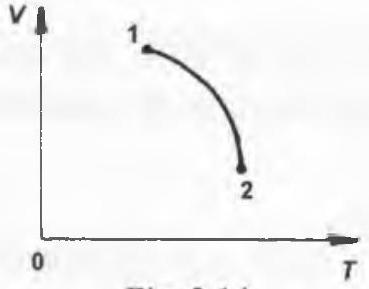
\includegraphics[max width=\textwidth, center]{2025_07_01_5b3ff9fa0d508c8e9f17g-098} Fig. 2.14\\

2.114. Cunoscând presiunea $p=55 \mathrm{~kPa}$ şi viteza pătratică medie a moleculelor de azot $v_{T}=550 \mathrm{~m} / \mathrm{s}$, concentrația moleculelor şi densitatea gazului sunt:\\ A) $n=10^{25} \mathrm{~m}^{-3} , \rho=0,465 \mathrm{~kg} / \mathrm{m}^{3}$; B) $n=10^{4} \mathrm{~m}^{-3} , \rho=0,500 \mathrm{~kg} / \mathrm{m}^{3}$; C) $n=5 \cdot 10^{25} \mathrm{~m}^{-3} , \rho=0,290 \mathrm{~kg} / \mathrm{m}^{3}$; D) $n=10^{25} \mathrm{~m}^{-3} , \rho=0,545 \mathrm{~kg} / \mathrm{m}^{3}$; E) $n=1,2 \cdot 10^{25} \mathrm{~m}^{3} , \rho=0,549 \mathrm{~kg} / \mathrm{m}^{3}$; F) $n=10^{-24} \mathrm{~m}^{3} , \rho=0,455 \mathrm{~kg} / \mathrm{m}^{3}$.\\ (Elena Slavnicu)\\

2.115. Două baloane legate printr-un tub subțire, prevăzut cu un robinet, conțin aer la aceeaşi temperatură. Volumul primului balon este de $n$ ori mai mare decât volumul celui de-al doilea. Presiunea în primul balon este $4 \cdot 10^{4} \mathrm{~N} / \mathrm{m}^{2}$. Masa aerului din balonul al doilea este de $k$ ori mai mare decât în primul. Presiunea care se stabileşte în baloane, dacă deschidem robinetul, este (se dau $n=3,5 ; k=4$ ):\\ A) $180 \mathrm{~kPa}$; B) $170 \mathrm{~N} / \mathrm{m}^{2}$; C) $155,6 \mathrm{kN} / \mathrm{m}^{2}$; D) $720 \mathrm{~N} / \mathrm{m}^{2}$; E) $72 \mathrm{~N} / \mathrm{m}^{2}$; F) $175 \mathrm{~kPa}$.\\ (Elena Slavnicu)\\

2.116. Două gaze diferite aflate la temperaturi diferite sunt în contact termic şi izolate de exterior. În acest caz, care din următoarele afirmații este adevărată:\\ A) gazele vor rămâne la temperaturi diferite; B) gazele vor ajunge la aceeaşi densitate; C) gazele vor ajunge la aceeaşi concentrație a moleculelor; D) gazele vor ajunge la aceeaşi energie cinetică medie de translație a unei molecule; E) gazele vor ajunge la aceeaşi viteză pătratică medie a moleculelor; F) nici una din variantele anterioare nu este corectă.\\ (Elena Slavnicu)\\

2.117. Care din următoarele afirmații este în contradicție cu principiul al doilea al termodinamicii?\\ A) lucrul mecanic se poate transforma integral în căldură; B) randamentul maxim al unui motor termic este subunitar; C) căldura se poate transforma integral în lucru mecanic, într-un proces ciclic, reversibil; D) nu este posibilă o transformare care să aibă ca rezultat trecerea căldurii de la un corp cu o temperatură dată, la altul de aceeaşi temperatură; E) se poate construi o maşină care să transforme căldura în lucru mecanic; F) într-o transformare ciclică, monotermă, sistemul nu poate ceda lucru mecanic în exterior.\\ (Elena Slavnicu)\\

2.118. Un mol de gaz ideal monoatomic se răceşte izocor astfel încât presiunea scade de $k$ ori, apoi gazul se destinde izobar astfel încât volumul său creşte de $k$ ori. Să se găsească valoarea lui $k$ dacă în aceste transformări s-a transmis gazului o căldură egală cu jumătate din energia internă inițială a gazului.\\ A) $k=1 / 2$; B) $k=8$; C) $k=4$; D) $k=3$; E) $k=2$; F) $k=\sqrt{2}$.\\ (Elena Slavnicu)\\

2.119. Un gaz închis într-o incintă de volum $V$, aflat la temperatura $T=300 \mathrm{~K}$ şi presiunea $p=2 \mathrm{~atm}$, suferă un proces termodinamic în urma căruia temperatura scade cu $\Delta T=30 \mathrm{~K}$ iar volumul creşte cu $n=20 \%$. Presiunea finală va fi:\\ A) $p=3 \mathrm{~atm}$; B) $p=1,5 \mathrm{~atm}$; C) $p=4 \mathrm{~atm}$; D) $p=3,5 \mathrm{~atm}$; E) presiunea rămâne neschimbată; F) $p=3,6 \mathrm{~atm}$.\\ (Constantin Roşu)\\

2.120. Un gaz ideal biatomic parcurge ciclul din Fig. 2.15. Ştiind că $V_{2}=e \cdot V_{1} \quad$ şi $\quad T_{3}=2 \cdot T_{2}$ ($e$ este baza logaritmilor naturali), să se calculeze randamentul ciclului.\\ A) $\eta=\frac{2}{5}$; B) $\eta=\frac{2}{9}$; C) $\eta=50 \%$; D) $\eta=\frac{3}{5}$; E) $\eta=\frac{1}{4}$; F) $\eta=\frac{3}{4}$.\\ (Constantin Roşu)\\ 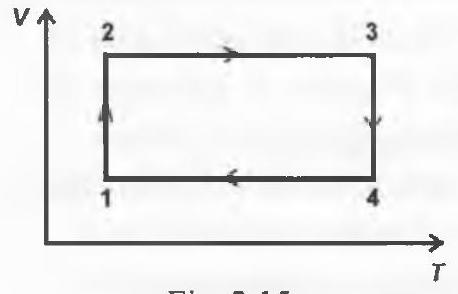
\includegraphics[max width=\textwidth, center]{2025_07_01_5b3ff9fa0d508c8e9f17g-100} Fig. 2.15\\

2.121. Un motor termic cu randamentul $\eta_{1}$ acționează un dinam cu puterea utilă $P$ şi randamentul $\eta_{2}$. Să se calculeze căldura oferită de motorul termic sistemului său de răcire în timpul $t$.\\ A) $Q_{\text {racire }}=\frac{P \cdot t \cdot\left(1+\eta_{1}\right)}{\eta_{1} \cdot \eta_{2}}$; B) $Q_{\text {racire }}=\frac{P \cdot t \cdot \eta_{1} \cdot \eta_{2}}{\eta_{1}+\eta_{2}}$; C) $Q_{\text {racire }}=\frac{(P-t)}{\eta_{1} \cdot \eta_{2}}$; D) $Q_{\text {racire }}=\frac{P \cdot t \cdot \sqrt{\eta_{1}}}{\eta_{1} \cdot \eta_{2}}$; E) $Q_{\text {racire }}=\frac{P \cdot t \cdot\left(1-\eta_{1}\right)}{\eta_{1} \cdot \eta_{2}}$; F) $Q_{\text {racire }}=\frac{P \cdot t \cdot\left(1-\eta_{1}\right)}{2 \eta_{1} \cdot \eta_{2}}$.\\ (Constantin Roşu)\\

2.122. Se pun în contact termic 4 corpuri din acelaşi material de temperaturi inițiale $t_{1}=10^{\circ} \mathrm{C}, t_{2}=20^{\circ} \mathrm{C}, t_{3}=30^{\circ} \mathrm{C}, t_{4}=50^{\circ} \mathrm{C}$ şi mase $m_{1}=2 \mathrm{~kg}, m_{2}=0,5 \mathrm{~kg}$, $m_{3}=I \mathrm{~kg}$ şi $m_{4}=3 \mathrm{~kg}$. Atunci temperatura finală a amestecului va fi:\\ A) $t=27,5^{\circ} \mathrm{C}$; B) $t=41,8^{\circ} \mathrm{C}$; C) $t=32,3{ }^{\circ} \mathrm{C}$; D) $t=56^{\circ} \mathrm{C}$; E) $t=42,4^{\circ} \mathrm{C}$; F) $t=22,5^{\circ} \mathrm{C}$.\\ (Constantin Roşu)\\

2.123. Un perpetuum mobile de speța I reprezintă:\\ A) o maşină termică care produce lucru mecanic de la o singură sursă de căldură; B) un motor Carnot; C) un motor care funcționează cu energie nucleară; D) o maşină termică care efectuează lucru mecanic fără consum de energie din exterior; E) o maşină termică bitermă; F) un ansamblu motor cu benzină plus dinam electric.\\ (Constantin Roşu)\\

2.124. Intre masa $m$ a unei molecule, masa molară $\mu$ a unui gaz constanta lui Boltzmann şi constanta gazelor perfecte $R$, există relația:\\ A) $\mu \cdot k=\sqrt{\frac{R}{m}}$; В) $\mu \cdot k=m \cdot R$; C) $\mu / k=m / R$; D) $\mu^{2}=m \cdot R / k$; E) $\mu+k=m-R$; F) $\mu / k=m \cdot R$.\\ (Constantin Roşu)\\

2.125. Lucrul mecanic efectuat de un sistem izolat adiabatic de exterior depinde numai de:\\ A) variația presiunii sistemului între starea inițială și finală; B) raportul dintre cāldura cedată şi primită de sistem; C) stările intermediare din prima jumătate a procesului; D) starea inițială şi finală a sistemului; E) logaritmul raportului dintre volumul final, respectiv inițial; F) temperatura sistemului, dar nu depinde de presiune.\\ (Constantin Roşu)\\

2.126. Într-un cilindru cu piston se află aer la presiunea $p_{1}=2 \cdot 10^{5} \mathrm{~N} / \mathrm{m}^{2}$ şi temperatura $T_{1}=300 \mathrm{~K}$. Să se afle masa unei greutăți care trebuie pusă deasupra pistonului, pentru ca volumul aerului să rămână constant, dacă gazul din piston este încălzit până la temperatura $T_{2}=333 \mathrm{~K}$. Secțiunea pistonului este $S=3 \cdot 10^{-3} \mathrm{~m}^{2}$. Se dă: $g=10 \mathrm{~m} / \mathrm{s}^{2}$.\\ A) $6,6 \mathrm{~g}$; B) $36 \mathrm{~kg}$; C) $6,6 \mathrm{~kg}$; D) $8 \mathrm{~kg}$; E) $4,6 \mathrm{~kg}$; F) $0,1 \mathrm{~kg}$.\\ (Răzvan Mitroi)\\

2.127. Să se afle căldurile specifice $c_{V}$ şi $c_{p}$ ale unui gaz ideal, ştiind masa moleculară $\mu=30 \mathrm{~kg} / \mathrm{kmol}$ şi coeficientul adiabatic $\gamma=1,4$. Se dă: $R=8,31 \mathrm{~J} / \mathrm{molK}$.\\ A) $c_{V}=692,5 \mathrm{~J} / \mathrm{kg} \cdot \mathrm{K}, c_{p}=692,5 \mathrm{~J} / \mathrm{kg} \cdot \mathrm{K}$; B) $c_{V}=250 \mathrm{~J} / \mathrm{kg} \cdot \mathrm{K}, c_{p}=692,5 \mathrm{~J} / \mathrm{kg} \cdot \mathrm{K}$; C) $c_{V}=692,5 \mathrm{~J} / \mathrm{kg} \cdot \mathrm{K}, c_{p}=969,5 \mathrm{~J} / \mathrm{kg} \cdot \mathrm{K}$; D) $c_{V}=392,5 \mathrm{~J} / \mathrm{kg} \cdot \mathrm{K}, c_{p}=372 \mathrm{~J} / \mathrm{kg} \cdot \mathrm{K}$; E) $c_{V}=392,5 \mathrm{~J} / \mathrm{kg} \cdot \mathrm{K}, c_{p}=692,5 \mathrm{~J} / \mathrm{kg} \cdot \mathrm{K}$; F) $c_{V}=30 \mathrm{~J} / \mathrm{kg} \cdot \mathrm{K}, c_{p}=38,31 \mathrm{~J} / \mathrm{kg} \cdot \mathrm{K}$.\\ (Răzvan Mitroi)\\

2.128. Într-un ciclu Carnot de randament $\eta=40 \%$, lucrul mecanic efectuat de gaz la destinderea izotermă este $L_{i z o t}=100 \mathrm{~J}$. Care este lucrul mecanic consumat de gaz la comprimarea izotermă ?\\ A) $60 \mathrm{~W}$; B) $100 \mathrm{~J}$; C) $260 \mathrm{~W}$; D) $50 \mathrm{~J}$; E) $60 \mathrm{~J}$; F) $6 \mathrm{~J}$.\\ (Rǎzvan Mitroi)\\

2.129. La ce temperatură viteza pătratică medie a moleculelor de azot se dublează față de valoarea de la temperatura $t_{0}=0^{\circ} \mathrm{C}$.\\ А) $1000 \mathrm{~K}$; B) $819^{\circ} \mathrm{C}$; C) $273 \mathrm{~K}$; D) $1000^{\circ} \mathrm{C}$; E) $500 \mathrm{~K}$; F) $100^{\circ} \mathrm{C}$.\\ (Rǎzvan Mitroi)\\

2.130. Ce masă de oxigen s-a consumat dintr-o butelie de volum $V=60 \mathrm{~litri}$ dacă presiunea inițială a fost $p_{1}=10^{7} \mathrm{~N} / \mathrm{m}^{2}$ la temperatura $t_{1}=27^{\circ} \mathrm{C}$, iar presiunea finala a devenit $p=29 \cdot 10^{5} \mathrm{~N} / \mathrm{m}^{2}$ la temperatura $t_{2}=17^{\circ} \mathrm{C}$. Se dau: $\mu_{\text {aer }}=32 \mathrm{~kg} / \mathrm{kmol}, R=8,31 \mathrm{~J} / \mathrm{mol} \cdot \mathrm{K}$.\\ A) $4,2 \mathrm{~kg}$; B) $5,39 \mathrm{~kg}$; C) $2 \mathrm{~kg}$; D) $1,8 \mathrm{~kg}$; E) $5,39 \mathrm{~g}$; F) $8 \mathrm{~kg}$.\\ (Răzvan Mitroi)\\

2.131. Un vas cilindric orizontal care este împărțit de un piston termoizolant, inițial blocat, în două părți de volume $V_{1}=1$ litru şi $V_{2}=2$ litri, conține gaz la presiunile $p_{1}=3 \cdot 10^{5} \mathrm{~N} / \mathrm{m}^{2}$ şi respectiv $p_{2}=10^{5} \mathrm{~N} / \mathrm{m}^{2}$ la aceeaşi temperatură. Pistonul este lăsat liber, iar gazul din primul compartiment este încălzit până la temperatura $T_{1}=400 \mathrm{~K}$, iar cel din al doilea compartiment este încălzit până la temperatura $T_{2}=300 \mathrm{~K}$. Cât va fi volumul fiecărui compartiment?\\ A) $2 \cdot 10^{-3} \mathrm{~m}^{3}, 2 \cdot 10^{-3} \mathrm{~m}^{3}$; B) $10^{-3} \mathrm{~m}^{3}, 4 \cdot 10^{-3} \mathrm{~m}^{3}$; C) $3 \cdot 10^{-3} \mathrm{~m}^{3}, 10^{-3} \mathrm{~m}^{3}$; D) $10^{-3} \mathrm{~m}^{3}, 10^{-3} \mathrm{~m}^{3}$; E) $2 \cdot 10^{-3} \mathrm{~m}^{3}, 10^{-3} \mathrm{~m}^{3}$; F) $3 \cdot 10^{-3} \mathrm{~m}^{3}, 7 \cdot 10^{-3} \mathrm{~m}^{3}$.\\ (Răzvan Mitroi)\\

2.132. Un balon având volumul $V=10^{-2} \mathrm{~m}^{3}$ contine oxigen la presiunea $p=10^{6} \mathrm{~N} / \mathrm{m}^{2}$ şi la temperatura $t=7^{\circ} \mathrm{C}$. Ce cantitate de căldură absoarbe gazul dacă este încălzit până la $17^{\circ} \mathrm{C}$, ştiind că densitatea oxigenului la $0^{\circ} \mathrm{C}$ este $1,43 \mathrm{~kg} / \mathrm{m}^{3}$, iar căldura specifică $921 \mathrm{~J} / \mathrm{kg} \cdot \mathrm{grad}$. Se va considera presiunea atmosfericǎ la $0^{\circ} \mathrm{C}, p_{0}=10^{5} \mathrm{~N} / \mathrm{m}^{2}$.\\ A) $280 \mathrm{~J}$; B) $100 \mathrm{~J}$; C) $1800 \mathrm{~J}$; D) $1280 \mathrm{~J}$; E) $500 \mathrm{~J}$; F) $640 \mathrm{~J}$.\\ (Răzvan Mitroi)\\

2.133. Într-un cilindru vertical cu piston se află aer la presiunea atmosferică normală $p_{0}=10^{5} \mathrm{~N} / \mathrm{m}^{2}$. Pistonul de masă neglijabilă şi secțiunea $S=200 \mathrm{~cm}^{2}$ se află inițial la distanța $d_{1}=1,6 \mathrm{~m}$ de fundul cilindrului, apoi este adus încet la distanța $d_{2}=10 \mathrm{~cm}$. Să se determine forța $F$ ce acționează asupra pistonului aflat în poziția finală. Frecările se neglijează.\\ A) $15 \mathrm{~N}$; B) $30 \mathrm{~N}$; C) $15 \mathrm{~kN}$; D) $30 \mathrm{~kN}$; E) $50 \mathrm{~N}$; F) $10 \mathrm{~kN}$.\\ (Tatiana Pop)\\

2.134. O masă $m=10 \mathrm{~g}$ de oxigen se află la presiunea $p=3 \cdot 10^{5} \mathrm{~N} / \mathrm{m}^{2}$ şi la temperatura $t_{1}=10^{\circ} \mathrm{C}$. După o încălzire izobară, gazul ocupă volumul $V_{2}=10 \mathrm{~litri}$. Cunoscând masa molară a oxigenului $\mu=32 \mathrm{~kg} / \mathrm{kmol}$, căldura molară izobară $C_{p}=7 R / 2$ şi constanta universală a gazelor perfecte $R=8310 \mathrm{~J} / \mathrm{kmol} \cdot \mathrm{K}$, atunci căldura absorbită de gaz şi variația energiei interne a gazului au valorile :\\ A) $Q=7927,8 \mathrm{~J}, \Delta U=5662,8 \mathrm{~J}$; B) $Q=5662,8 \mathrm{~J}, \Delta U=7927,8 \mathrm{~J}$; C) $Q=9727,8 \mathrm{~J}, \Delta U=2565,8 \mathrm{~J}$; D) $Q=7927,8 \mathrm{~J}, \Delta U=0$; E) $Q=0 \mathrm{~J}, \Delta U=0 \mathrm{~J}$; F) $Q=-79,275 \mathrm{~J}, \Delta U=56,65 \mathrm{~J}$.\\ (Tatiana Pop)\\

2.135. Randamentul unui ciclu format din două izobare şi două izocore cu $p=2 p_{0}$ şi $V_{1}=V_{0}$ şi $p_{3}=p_{0}$ şi $V_{3}=3 V_{0}$, parcurs de un gaz ideal biatomic cu $C_{V}=5 R / 2$ este:\\ A) $50 \%$; В) $36,4 \%$; C) $24,24 \%$; D) $12,12 \%$; E) $75 \%$; F) $1,2 \%$.\\ (Tatiana Pop)\\

2.136. Un mol de gaz ideal se găseşte în starea $A$, caracterizată prin temperatura $t_{A}=47^{\circ} \mathrm{C}$. Gazul trece într-o stare $B$, printr-o încălzire izobară producând un lucru mecanic $L=1662 \mathrm{~J}$. Se cere temperatura $T_{B}$ din starea finală, $R=8,31 \mathrm{~J} / \mathrm{mol} \cdot \mathrm{K}$.\\ A) $520 \mathrm{~K}$; В) $150 \mathrm{~K}$; C) $300 \mathrm{~K}$; D) $100 \mathrm{~K}$; E) $700 \mathrm{~K}$; F) $820 \mathrm{~K}$.\\ (Tatiana Pop)\\

2.137. Temperatura unui gaz scade izocor de la valoarea $T_{1}=400 \mathrm{~K}$ la $T_{2}=200 \mathrm{~K}$. Cu cât la sută scade presiunea gazului:\\ A) $10 \%$; B) $20 \%$; C) $70 \%$; D) $45 \%$; E) $50 \%$; F) $30 \%$.\\ (Ion Belciu)\\

2.138. O maşină termică funcționând după un ciclu Carnot între temperaturile $T_{1}=400 \mathrm{~K}$ şi $T_{2}=300 \mathrm{~K}$, produce într-un ciclu lucrul mecanic $L=80 \mathrm{~kJ}$. Căldura cedată sursei reci într-un ciclu este:\\ A) $100 \mathrm{~kJ}$; B) $250 \mathrm{~kJ}$; C) $40 \mathrm{~kJ}$; D) $240 \mathrm{~kJ}$; E) $120 \mathrm{~kJ}$; F) $152 \mathrm{~kJ}$.\\ (Ion Belciu)\\

2.139. O maşină termică funcționează cu gaz ideal biatomic ( $C_{V}=\frac{5}{2} R$ ) după ciclul din Fig. 2.16. Randamentul maşinii termice este:\\ A) $\frac{2}{3}$; B) $\frac{15}{40}$; C) $\frac{16}{30}$; D) $\frac{20}{75}$; E) $\frac{2}{13}$; F) $\frac{5}{17}$.\\ (Ion Belciu)\\ 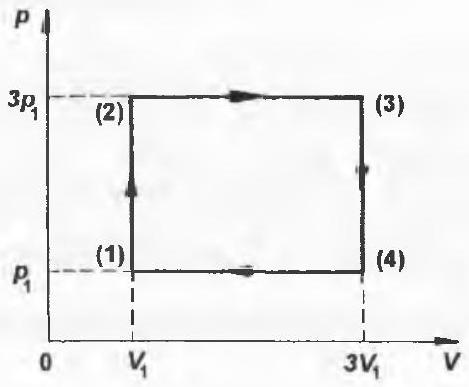
\includegraphics[max width=\textwidth, center]{2025_07_01_5b3ff9fa0d508c8e9f17g-104} Fig. 2.16\\

2.140. O pompă de vid de volum $V_{0}$ trebuie să micşoreze presiunea aerului dintr-un vas cu volumul $V$ de la presiunea $p_{0}$ la presiunea $p=10^{-4} p_{0}$. Considerând temperatura constantă, numărul curselor făcute de pompă va fi:\\ A) $10^{-4} \frac{p}{p_{0}}$; B) $10^{-4} \frac{V_{0}+V}{V}$; C) $\frac{\lg \left(\frac{V+V_{0}}{V}\right)}{5}$; D) $4 \ln \frac{V_{0}}{V}$; E) $\frac{4}{\lg \left(\frac{V+V_{0}}{V}\right)}$; F) $4 \frac{p_{0}}{p}$.\\ (Ion Belciu)\\

2.141. Presiunea unui gaz creşte de patru ori prin încălzire izocoră. Raportul vitezelor termice ale moleculelor de gaz înainte şi după încălzire este:\\ А) 4; B) 2; C) $\frac{1}{4}$; D) $\frac{1}{2}$; E) $\frac{1}{16}$; F) $\frac{1}{5}$.\\ (Ion Belciu)\\

2.142. O bară de oțel cu secţiunea $S=10 \mathrm{~cm}^{2}$, având modulul de elasticitate $E=2 \cdot 10^{11} \mathrm{~N} / \mathrm{m}^{2}$ şi coeficientul de dilatare volumică $\gamma=33 \cdot 10^{-6} \mathrm{~K}^{-1}$, este fixată la capete de un suport rigid. Crescând temperatura barei cu $\Delta T=100 \mathrm{~K}$, forța cu care apasă bara asupra suportului va fi:\\ A) $10^{9} \mathrm{~N}$; B) $3 \cdot 10^{10} \mathrm{~N}$; C) $27 \cdot 10^{8} \mathrm{~N}$; D) $22 \cdot 10^{4} \mathrm{~N}$; E) $3 \cdot 10^{7} \mathrm{~N}$; F) $52 \cdot 10^{5} \mathrm{~N}$.\\ (Ion Belciu)\\

2.143. Se amestecă o cantitate de apă cu temperatura $t_{1}=40^{\circ} \mathrm{C}$ cu o cantitate triplă de apă cu temperatura $t_{2}=60^{\circ} \mathrm{C}$. Temperatura finală a amestecului de apă va fi:\\ A) $42^{\circ} \mathrm{C}$; B) $50^{\circ} \mathrm{C}$; C) $30^{\circ} \mathrm{C}$; D) $55^{\circ} \mathrm{C}$; E) $58^{\circ} \mathrm{C}$; F) $45^{\circ} \mathrm{C}$.\\ (Ion Belciu)\\

2.144. În interiorul unui cilindru orizontal, izolat adiabatic față de exterior, se găseşte în compartimentul A (Fig. 2.17) o cantitate $\nu$ dintr-un gaz ideal la temperatura $t_{\mathrm{A}}=127^{\circ} \mathrm{C}$, ocupând un volum delimitat de peretele fix $M$, ce permite schimbul de căldură cu compartimentul $B$, în care se găseşte aceeaşi cantitate $\nu$ din acelaşi gaz, la presiunea atmosferică $p_{0}$ şi temperatura inițială $t_{\mathrm{B}}=27^{\circ} \mathrm{C}$, volumul acestui compartiment fiind variabil prin deplasarea pistonului $P$ ce se poate mişca fară frecare. În exteriorul cilindrului presiunea aerului este $p_{0}$, iar căldura molară la volum constant a gazului din compartimentele A şi B este $\frac{3}{2} R$. După un timp se ajunge la echilibru termodinamic, temperatura din ambele compartimente fiind $T_{f}$ :\\ А) $387,5 \mathrm{~K}$; В) $350 \mathrm{~K}$; C) $337,5 \mathrm{~K}$; D) $327,5 \mathrm{~K}$; E) $316 \mathrm{~K}$; F) $302,5 \mathrm{~K}$.\\ (Corneliu Călin)\\ 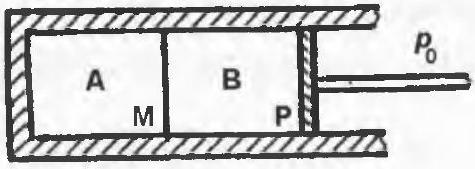
\includegraphics[max width=\textwidth, center]{2025_07_01_5b3ff9fa0d508c8e9f17g-105} Fig. 2.17\\

2.145. Prin încălzirea masei $m=2 \cdot 10^{-3} \mathrm{~kg}$ de gaz ideal diatomic, viteza termică a crescut de la $v_{T_{1}}=400 \mathrm{~m} / \mathrm{s}$ la $v_{T_{2}}=500 \mathrm{~m} / \mathrm{s}$. Se cere variația energiei interne a cantității respective de gaz, ştiind $C_{V}=\frac{5}{2} R$.\\ A) $225 \mathrm{~J}$; B) $360 \mathrm{~J}$; C) $150 \mathrm{~J}$; D) $600 \mathrm{~J}$; E) $900 \mathrm{~J}$; F) $1200 \mathrm{~J}$.\\ (Corneliu Călin)\\

2.146. Procesul ciclic efectuat de o cantitate de gaz ideal monoatomic se reprezintă (Fig. 2.18) prin dreapta 1-2 (a cărei prelungire trece prin 0), prin izocora $2-3$ urmată de izobara $3-1$. Ştiind căldura molară în transformarea $1-2$ : $C_{12}=2 R$ şi raportul $\frac{V_{2}}{V_{1}}=2$, se cere randamentul $\eta$ al acestui ciclu şi randamentul $\eta_{c}$ al unui ciclu Carnot care ar evolua între aceleaşi limite extreme de temperaturi:\\ A) $\eta=\frac{1}{12}, \eta_{c}=\frac{3}{4}$; B) $\eta=\frac{1}{6}, \eta_{c}=\frac{3}{4}$; C) $\eta=\frac{2}{3}, \eta_{c}=\frac{3}{4}$; D) $\eta=\frac{1}{8}, \eta_{c}=\frac{1}{2}$; E) $\eta=\frac{1}{6}, \eta_{c}=\frac{1}{2}$; F) $\eta=\frac{1}{3}, \eta_{c}=\frac{2}{3}$.\\ (Corneliu Călin)\\ 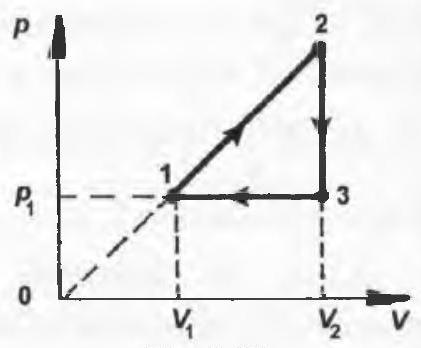
\includegraphics[max width=\textwidth, center]{2025_07_01_5b3ff9fa0d508c8e9f17g-106} Fig. 2.18\\

2.147. Cantitatea de $1 \mathrm{~kmol}$ de gaz ideal efectuează un ciclu Carnot între temperaturile $t_{1}=227^{\circ} \mathrm{C}$ şi $t_{2}=27^{\circ} \mathrm{C}$, raportul volumelor în procesul destinderii izoterme find $\varepsilon=10$. Se cere lucrul mecanic efectuat în cursul ciclului. Se consideră constanta gazelor $R=8,31 \mathrm{~J} / \mathrm{mol} \mathrm{K}$.\\ A) $3,818 \mathrm{~MJ}$; B) $9,545 \mathrm{~MJ}$; C) $5,727 \mathrm{~MJ}$; D) $3,818 \mathrm{~kJ}$; E) $9,545 \mathrm{~kJ}$; F) $5,725 \mathrm{~kJ}$.\\ (Corneliu Călin)\\

2.148. Într-o incintă se află azot la presiunea $p=10^{5} \mathrm{~Pa}$. Care este concentrația moleculelor de azot dacă viteza pătratică medie a acestora este $v=10^{4} \mathrm{~m} / \mathrm{s}$ ?\\ A) $1,5 \cdot 10^{15} \mathrm{~m}^{-3}$; B) $\frac{3}{5} \cdot 10^{20} \mathrm{~m}^{-3}$; C) $\frac{9}{14} \cdot 10^{23} \mathrm{~m}^{-3}$; D) $7 \cdot 10^{22} \mathrm{~m}^{-3}$; E) $\frac{8}{3} \cdot 10^{18} \mathrm{~m}^{-3}$; F) $10^{24} \mathrm{~m}^{-3}$.\\ (Marin Cilea)\\

2.149. Intr-o butelie de volum $V=83,1 \mathrm{~litri}$ se aflã heliu la presiunea $p=2,9 \cdot 10^{5} \mathrm{~Pa}$ şi temperatura $T_{1}=290 \mathrm{~K}$. După ce din butelie s-a mai scos heliu, presiunea a devenit $p_{2}=1,25 \cdot 10^{5} \mathrm{~Pa}$, iar temperatura $T_{2}=250 \mathrm{~K}$. Cu cât a scăzut masa heliului din butelie?\\ A) $15 \mathrm{~g}$; B) $1,5 \mathrm{~g}$; C) $100 \mathrm{~g}$; D) $20 \mathrm{~g}$; E) $85 \mathrm{~g}$; F) $44 \mathrm{~g}$.\\ (Marin Cilea)\\

2.150. O masă de azot $m=6,73 \mathrm{~g}$ este încălzită cu $\Delta T=200 \mathrm{~K}$ la volum constant. Să se afle căldura $Q_{V}$ absorbită $\left(C_{V}=\frac{5}{2} R\right)$.\\ A) $100 \mathrm{~J}$; B) $2500 \mathrm{~J}$; C) $1000 \mathrm{~J}$; D) $4 \mathrm{~kJ}$; E) $2,2 \mathrm{~kJ}$; F) $200 \mathrm{~J}$.\\ (Marin Cilea)\\

2.151. Un gaz ocupă volumul $V_{1}=10^{-2} \mathrm{~m}^{3}$ la presiunea $p_{1}=2,9 \cdot 10^{5} \mathrm{~Pa}$ şi temperatura $T_{1}=290 \mathrm{~K}$. Gazul este încǎlzit izobar şi efectuează un lucru mecanic $L=200 \mathrm{~J}$. Să se afle cu cât s-a încălzit gazul.\\ A) $20 \mathrm{~K}$; B) $10 \mathrm{~K}$; C) $100 \mathrm{~K}$; D) $45 \mathrm{~K}$; E) $550 \mathrm{~K}$; F) $300 \mathrm{~K}$.\\ (Marin Cilea)\\

2.152. Într-un recipient de volum $V=2 \cdot 10^{-2} \mathrm{~m}^{3}$ se află hidrogen la presiunea $p_{1}=10^{5} \mathrm{~Pa}$. Gazul este încălzit la volum constant până când presiunea sa devine $P_{2}=2 \cdot 10^{5} \mathrm{~Pa}$. Să se afle variația energiei interne $\left(C_{V}=\frac{5}{2} R\right)$.\\ A) $2 \mathrm{~kJ}$; B) $5 \cdot 10^{3} \mathrm{~J}$; C) $4 \mathrm{~kJ}$; D) $12,1 \mathrm{~kJ}$; E) $200 \mathrm{~J}$; F) $800 \mathrm{~J}$.\\ (Marin Cilea)\\

2.153. Un gaz efectuează o transformare ciclică în timpul căreia primeşte de la sursa caldă căldura $Q_{1}=4 \mathrm{~kJ}$. Să se afle lucrul mecanic efectuat de gaz într-un ciclu dacã randamentul acestuia este $\eta=0,25$.\\ A) $750 \mathrm{~J}$; B) $1 \mathrm{~kJ}$; C) $3 \mathrm{~kJ}$; D) $1,2 \mathrm{~kJ}$; E) $950 \mathrm{~J}$; F) $500 \mathrm{~J}$.\\ (Marin Cilea)\\

2.154. Într-un kilogram de apă cu temperatura de $10^{\circ} \mathrm{C}$ se pun $4,181 \mathrm{~kg}$ dintr-un metal cu temperatura de $80^{\circ} \mathrm{C}$. Temperatura de echilibru a amestecului este de $40^{\circ} \mathrm{C}$. Care este căldura specifică a metalului? ( $c_{\text {apă }}=4181 \mathrm{~J} / \mathrm{kg} \cdot \mathrm{K}$ )\\ A) $225 \mathrm{~J} / \mathrm{kg} \cdot \mathrm{K}$; B) $410 \mathrm{~J} / \mathrm{kg} \cdot \mathrm{K}$; C) $10^{3} \mathrm{~J} / \mathrm{kg} \cdot \mathrm{K}$; D) $750 \mathrm{~J} / \mathrm{kg} \cdot \mathrm{K}$; E) $550 \mathrm{~J} / \mathrm{kg} \cdot \mathrm{K}$; F) $760 \mathrm{~J} / \mathrm{kg} \cdot \mathrm{K}$.\\ (Marin Cilea)\\

2.155. Într-un cilindru orizontal ìmpărțit în două compartimente (cu ajutorul unui piston care se poate mişca făă frecări) se găsesc două cantități de gaze diferite $m_{1}$, respectiv $m_{2}$, de mase molare $\mu_{1}$ şi $\mu_{2}$, la temperaturile $T_{1}$ şi $T_{2}$. Raportul volumelor este:\\ A) $\frac{V_{1}}{V_{2}}=\frac{m_{1}}{m_{2}} \cdot \frac{T_{1}}{T_{2}} \cdot \frac{\mu_{1}}{\mu_{2}}$; В) $\frac{V_{1}}{V_{2}}=\frac{m_{2}}{m_{1}} \cdot \frac{T_{2}}{T_{1}} \cdot \frac{\mu_{1}}{\mu_{2}}$; C) $\frac{V_{1}}{V_{2}}=\frac{m_{2}}{m_{1}} \cdot \frac{T_{1}}{T_{2}} \cdot \frac{\mu_{2}}{\mu_{1}}$; D) $\frac{V_{1}}{V_{2}}=\frac{m_{1}}{m_{2}} \cdot \frac{T_{1}}{T_{2}} \cdot \frac{\mu_{2}}{\mu_{1}}$; E) $\frac{V_{1}}{V_{2}}=\frac{m_{1}}{m_{2}} \cdot \frac{T_{2}}{T_{1}} \cdot \frac{\mu_{1}}{\mu_{2}}$; F) $\frac{V_{1}}{V_{2}}=\frac{m_{1}}{m_{2}} \cdot \frac{T_{2}}{T_{1}} \cdot \frac{\mu_{2}}{\mu_{1}}$.\\ (Ilie Ivanov)\\

2.156. Un recipient de volum $V$ conține gaz la presiunea $p_{0}$ şi la temperatura $T_{1}$. Dacă se încălzeşte sistemul până la o temperatură $T_{2}>T_{1}$, iese afară o masă $\Delta m$ care asigură menținerea unei presiuni $p=p_{0}$. Densitatea $\rho_{0}$ a gazului în condiții normale se exprimă prin relația:\\ A) $\rho_{0}=\frac{\Delta m\left(T_{2}-T_{1}\right)}{T_{1} T_{0} V}$; B) $\rho_{0}=V \Delta m$; C) $\rho_{0}=\frac{T_{1} T_{2} \Delta m}{\sqrt{T_{0}}\left(T_{2}-T_{1}\right)}$; D) $\rho_{0}=\frac{2 T_{1} T_{2} \Delta m}{\left(T_{1}+T_{2}\right) V T_{0}}$; E) $\rho_{0}=\frac{\Delta m\left(T_{1}-T_{2}\right)}{T_{1} T_{0} V}$; F) $\rho_{0}=\frac{T_{0}\left(T_{1}-T_{2}\right)}{T_{1} T_{2}} \frac{\Delta m}{V}$.\\ (Ilie Ivanov)\\

2.157. Un mol de He dintr-un recipient de volum $V=22 \mathrm{~litri}$ este încălzit cu $\Delta T=10 \mathrm{~K}$ presiunea crescând de 10 ori. Temperatura inițială $T_{1}$ este:\\ A) $11 \mathrm{~K}$; В) $0,1 \mathrm{~K}$; C) $1,1 \mathrm{~K}$; D) $111 \mathrm{~K}$; E) $2,2 \mathrm{~K}$; F) $22 \mathrm{~K}$.\\ (Ilie Ivanov)\\

2.158. Într-un recipient izolat adiabatic de mediul exterior se găsesc două gaze monoatomice ideale, separate printr-un perete adiabatic. Temperaturile lor sunt $T_{1}$, respectiv $T_{2}$, iar cantitățile de substanță $\nu_{1}$, respectiv $\nu_{2}$. Dacă se scoate peretele dintre ele sau dacă acesta este poros, atunci în urma difuziei temperatura de echilibru va fi:\\ A) $T=\frac{\nu_{1} T_{1}+\nu_{2} T_{2}}{2 \sqrt{\nu_{1} \nu_{2}}}$; B) $T=\sqrt{T_{1} T_{2}} \sqrt{\frac{\nu_{1} \nu_{2}}{\nu_{1}+\nu_{2}}}$; C) $T=\frac{\nu_{1} T_{1}+\nu_{2} T_{2}}{\nu_{1}+\nu_{2}}$; D) $T=\frac{2 \nu_{1} \nu_{2}}{\nu_{1}+\nu_{2}} \cdot \frac{T_{1}+T_{2}}{2}$; E) $T=\frac{\nu_{1} T_{2}+\nu_{2} T_{1}}{\nu_{1}+\nu_{2}}$; F) $\left(\frac{1}{\nu_{1}}+\frac{1}{\nu_{2}}\right) \cdot \frac{T_{1} T_{2}}{T_{1}+T_{2}}\left(\nu_{1}+\nu_{2}\right)$.\\ (Ilie Ivanov)\\

2.159. Într-un vas de sticlă cu coeficientul de dilatație volumică $\gamma$ se găseşte o masă de apă $m$ atunci când este plin la temperatura $t_{0}=0^{\circ} \mathrm{C}$. Prin încălzire până la temperatura $t$, o parte din lichid curge şi rămâne masa $m^{\prime}<m$. Se cere coeficientul de dilatare volumică al apei, $\gamma_{a}$.\\ A) $\gamma_{a}=\gamma$; B) $\gamma_{a}=\gamma \frac{m-m^{\prime}}{m^{\prime}}$; C) $\gamma_{a}=\gamma \frac{m \gamma t-m^{\prime}}{m^{\prime} t}$; D) $\gamma_{a}=\frac{m-m^{\prime}+m \gamma t}{m^{\prime} t}$; E) $\gamma_{a}=\frac{\left(m-m^{\prime}\right) y t-m^{\prime}}{m t}$; F) $\gamma_{a}=\gamma \frac{m-m^{\prime}}{m}$.\\ (Ilie Ivanov)\\

2.160. În care dintre procesele reprezentate in Fig. 2.19 lucrul mecanic schimbat de sistem (gaz ideal) este cel mai mic? Toate procesele au loc între aceleaşi stări, notate cu 1 (inițială) şi 2 (finală).\\ A) în a; B) în b; C) în c; D) în d; E) în e; F) în toate procesele lucrul mecanic este acelaşi.\\ (Eugen Scarlat)\\ 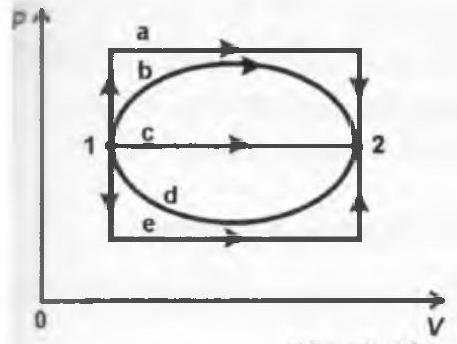
\includegraphics[max width=\textwidth, center]{2025_07_01_5b3ff9fa0d508c8e9f17g-109(1)} Fig. 2.19\\

2.161. În care dintre procesele reprezentate în Fig. 2.20, variația energiei interne este cea mai mică? Toate procesele au loc între starea inițială 1 şi starea finală 2.\\ A) în a; B) în b; C) în c; D) în d; E) în e; F) în toate procesele variația energiei interne este aceeaşi.\\ (Eugen Scarlat)\\ 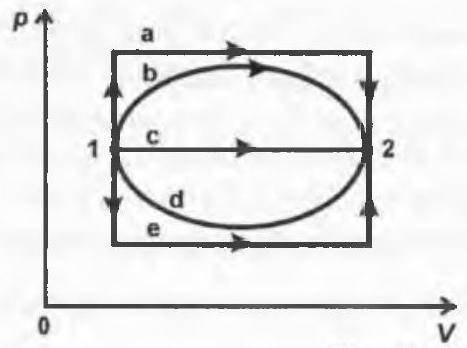
\includegraphics[max width=\textwidth, center]{2025_07_01_5b3ff9fa0d508c8e9f17g-109} Fig. 2.20\\

2.162. În care dintre transformările izobare, reprezentate în Fig. 2.21, ale unei cantități fixate de gaz ideal, presiunea este cea mai mică? În toate stările inițiale temperatura este $T_{1}$ şi în toate stările finale temperatura este $T_{2}$.\\ A) în a; B) în b; C) în c; D) în d; E) în e; F) în toate procesele reprezentate presiunea este aceeaşi.\\ (Eugen Scarlat)\\ 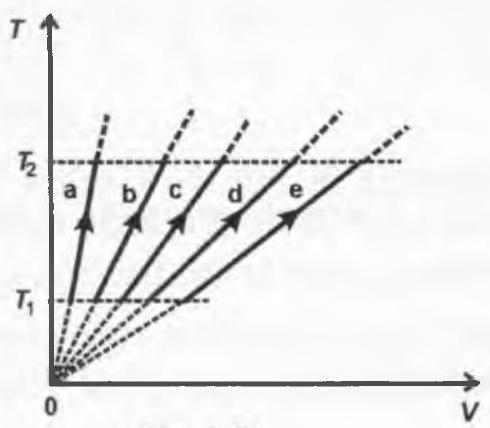
\includegraphics[max width=\textwidth, center]{2025_07_01_5b3ff9fa0d508c8e9f17g-110(3)} Fig. 2.21\\

2.163. În care dintre transformǎrile izocore, reprezentate în Fig. 2.22, ale unei cantități fixate de gaz ideal, volumul este cel mai mic? În toate stările inițiale temperatura este $T_{1}$ şi în toate stările finale temperatura este $T_{2}$.\\ A) în a; B) în b; C) în c; D) în d; E) în e; F) în toate procesele reprezentate volumul este acelaşi.\\ (Eugen Scarlat)\\ 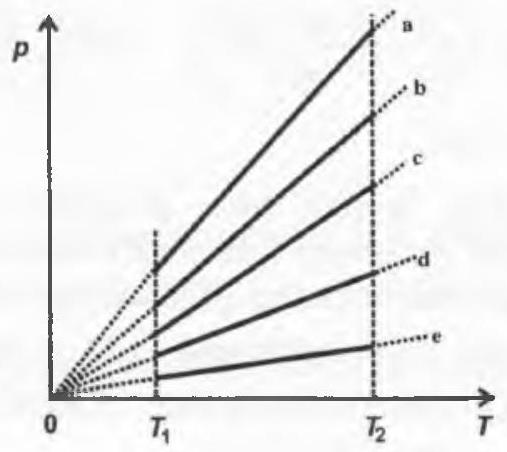
\includegraphics[max width=\textwidth, center]{2025_07_01_5b3ff9fa0d508c8e9f17g-110(2)} Fig. 2.22\\

2.164. În care dintre transformările reprezentate în Fig. 2.23, ale unei cantități fixate de gaz ideal, variația energiei interne este cea mai mică? În toate stările inițiale temperatura este $T_{1}$ şi în toate stările finale temperatura este $T_{2}$.\\ A) în a; B) în b; C) în c; D) în d; E) în e; F) în toate procesele reprezentate variația energiei interne este aceeaşi.\\ (Eugen Scarlat)\\ 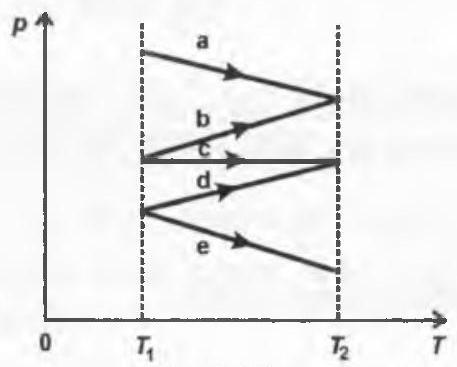
\includegraphics[max width=\textwidth, center]{2025_07_01_5b3ff9fa0d508c8e9f17g-110} Fig. 2.23\\

2.165. În care dintre procesele reprezentate în Fig. 2.24 căldura schimbată de sistem (gaz ideal) este cea mai mică? Toate procesele au loc între aceleaşi stări, notate cu 1 (inițială) şi 2 (finală).\\ A) în a; B) în b; C) în c; D) în d; E) în e; F) în toate procesele reprezentate căldura schimbată este aceeaşi.\\ (Eugen Scarlat)\\ 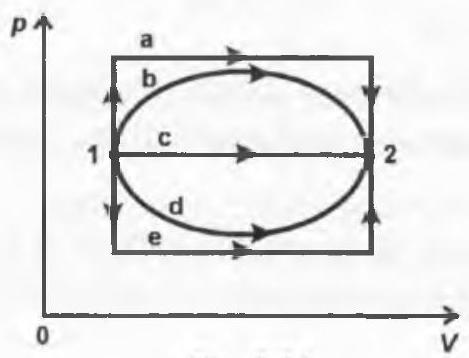
\includegraphics[max width=\textwidth, center]{2025_07_01_5b3ff9fa0d508c8e9f17g-110(1)} Fig. 2.24\\

2.166. În care dintre procesele reprezentate în Fig. 2.25 căldura schimbată de sistem (gaz ideal) este cea mai mică? Toate procesele au loc între aceleaşi stări, potate cu 1 (initială) şi 2 (finală).\\ A) în a; B) în b; C) în c; D) în d; E) în e; F) în toate procesele reprezentate căldura schimbată este aceeaşi.\\ (Eugen Scarlat)\\ 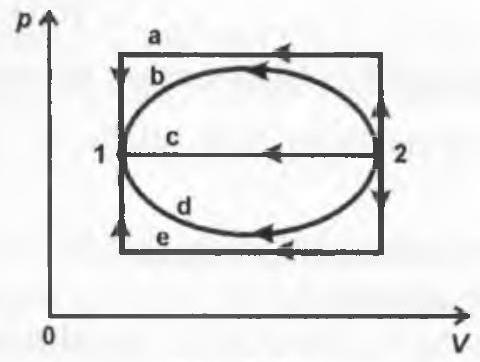
\includegraphics[max width=\textwidth, center]{2025_07_01_5b3ff9fa0d508c8e9f17g-111} Fig. 2.25\\

2.167. În care dintre procesele reprezentate în Fig. 2.26 lucrul mecanic schimbat de sistem (gaz ideal) este cel mai mic? Toate procesele au loc între aceleaşi stări, notate cu 1 (inițială) şi 2 (finală).\\ A) în a; B) în b; C) în c; D) în d; E) în e; F) în toate procesele reprezentate lucrul mecanic schimbat este acelaşi.\\ (Eugen Scarlat)\\ 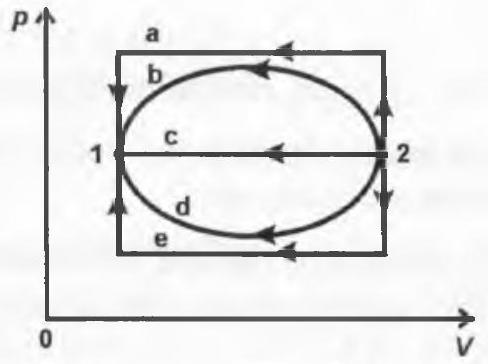
\includegraphics[max width=\textwidth, center]{2025_07_01_5b3ff9fa0d508c8e9f17g-111(1)} Fig. 2.26\\

2.168. Într-un gram de dioxid de carbon există un număr de molecule egal cu:\\ А) $1,36 \times 10^{20}$; В) $3.61 \times 10^{21}$; C) $1,36 \times 10^{22}$; D) $6,31 \times 10^{22}$; E) $3,61 \times 10^{22}$; F) $6,023 \times 10^{23}$.\\ (Mihai Cristea)\\

2.169. Un gaz aflat în condiții normale de temperatură şi presiune, are densitatea $\rho=1,25 \mathrm{mg} / \mathrm{cm}^{3}$. Acest gaz este:\\ A) He; B) $\mathrm{H}_{2}$; C) $\mathrm{C}_{2} \mathrm{H}_{2}$; D) $\mathrm{N}_{2}$; E) $\mathrm{CO}_{2}$; F) $\mathrm{O}_{2}$.\\ (Mihai Cristea)\\

2.170. Un gaz ideal $\left(C_{V}=\frac{3}{2} R\right)$ suferă o destindere izobară. Lucrul mecanic efectuat în cursul acestui proces reprezintă un procent din căldura primită egal cu:\\ А) $40 \%$; B) $60 \%$; C) $80 \%$; D) $50 \%$; E) $20 \%$; F) $30 \%$.\\ (Mihai Cristea)\\

2.171. Un motor termic ce funcționează după un ciclu Carnot are randamentul $\eta=50 \%$. Un alt motor Carnot are temperatura sursei reci de două ori mai mare decât temperatura sursei reci a primului motor. Ştiind cǎ diferența dintre temperatura sursei calde şi temperatura sursei reci este aceeaşi în cazul ambelor motoare, atunci randamentul celui de-al doilea motor termic este:\\ A) $25 \%$; B) $33,33 \%$; C) $50 \%$; D) $66,66 \%$; Е) $75 \%$; F) $88,88 \%$.\\ (Mihai Cristea)\\

2.172. O masă constantă de gaz ideal suferă o transformare în care viteza pătratică medie depinde de concentrația particulelor prin relația $\overline{v^{2}} \cdot n=c t$. Această transformare este:\\ A) izotermă; B) izocoră; C) izobară; D) adiabatică; E) oarecare; F) nu reprezintă nici o transformare termodinamică.\\ (Mihai Cristea)\\

2.173. Un gaz ideal monoatomic parcurge ciclul din Fig. 2.27, unde transformarea $2 \rightarrow 3$ este adiabatică, iar transformarea $3 \rightarrow 1$ este izotermă. Știind că $V_{2}=\frac{V_{1}}{2}$, să se calculeze randamentul acestui ciclu în funcție de randamentul unui ciclu Carnot ce ar funcționa între temperaturile extreme atinse pe acest ciclu.\\ A) $\eta=1-\frac{\eta_{c}}{\ln \left(1-\eta_{c}\right)}$; B) $\eta=1-\frac{2 \eta_{c}}{\ln 2-\frac{3}{2} \ln \left(1-\eta_{c}\right)}$; C) $\eta=1-\frac{\eta_{c}}{2 \ln 2}$; D) $\eta=1-\frac{2 \ln \left(1+\eta_{c}\right)}{3 \ln 2}$; E) $\eta=\frac{1}{2} \eta_{c} ; \quad$ F) $\eta=1-\frac{\ln \left(1+\eta_{c}\right)}{\eta_{c}}$.\\ (Mihai Cristea)\\ 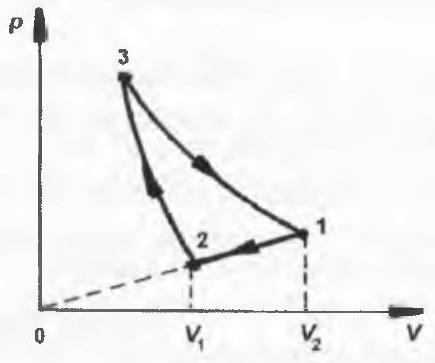
\includegraphics[max width=\textwidth, center]{2025_07_01_5b3ff9fa0d508c8e9f17g-112} Fig. 2.27\\

2.174. Un mol de gaz ideal monoatomic trece dintr-o stare 1 în starea finală 4 conform graficului din Fig. 2.28. Căldura totală schimbată de gaz cu mediul exterior, dacă diferența dintre temperatura finală şi cea inițială este de $\Delta T=100 \mathrm{~K}$. este egală cu ( $C_{V}=3 R / 2, R=8310 \mathrm{~J} / \mathrm{kmol} \mathrm{K}$ ):\\ A) $3 \mathrm{R} / 20 \mathrm{~J}$; B) $5 \mathrm{R} / 20 \mathrm{~J}$; C) $7 \mathrm{R} / 20 \mathrm{~J}$; D) $3 \mathrm{R} / 40 \mathrm{~J}$; E) $5 \mathrm{R} / 40 \mathrm{~J}$; F) $7 \mathrm{R} / 40 \mathrm{~J}$.\\ (Daniela Buzatu)\\ 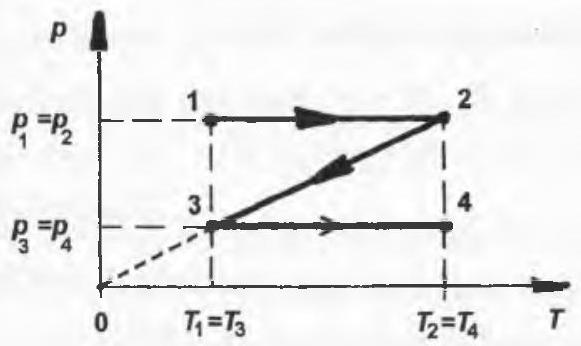
\includegraphics[max width=\textwidth, center]{2025_07_01_5b3ff9fa0d508c8e9f17g-113(1)} Fig. 2.28\\

2.175. Un gaz ideal monoatomic de masă $m=80 \mathrm{~g}$ şi masă molară $\mu=40 \mathrm{~g} / \mathrm{mol}$ este încălzit într-un cilindru cu piston, astfel încât temperatura lui variază proporțional cu pătratul presiunii $\left(T \sim p^{2}\right)$ de la valoarea inițială $T_{1}=300 \mathrm{~K}$ până la temperatura finalǎ $T_{2}=400 \mathrm{~K}$. Lucrul mecanic efectuat de gaz în timpul procesului şi cantitatea de căldură transmisă gazului au valorile ( $R=8310 \mathrm{~J} / \mathrm{kmol} \mathrm{K}$ ):\\ A) $380 \mathrm{~J} , 2,3 \mathrm{~kJ}$; B) $330 \mathrm{~J} , 3,6 \mathrm{~kJ}$; C) $730 \mathrm{~J} , 6,3 \mathrm{~kJ}$; D) $871 \mathrm{~J} , 4 \mathrm{~kJ}$; E) $831 \mathrm{~J} , 0,831 \mathrm{~kJ}$; F) $831 \mathrm{~J} , 3,324 \mathrm{~kJ}$.\\ (Daniela Buzatu)\\

2.176. În Fig. 2.29 sunt prezentate două cicluri închise: $1 \rightarrow 2 \rightarrow 3$ şi $1 \rightarrow 3 \rightarrow 4$. Amândouă ciclurile sunt efectuate de câte un mol de gaz ideal monoatomic. Calculați raportul randamentelor celor două cicluri $\eta(1 \rightarrow 2 \rightarrow 3) / \eta(1 \rightarrow 3 \rightarrow 4)$.\\ А) $22 / 20$; B) $25 / 24$; C) $24 / 23$; D) $24 / 22$; E) $21 / 23$; F) $25 / 23$.\\ (Daniela Buzatu)\\ 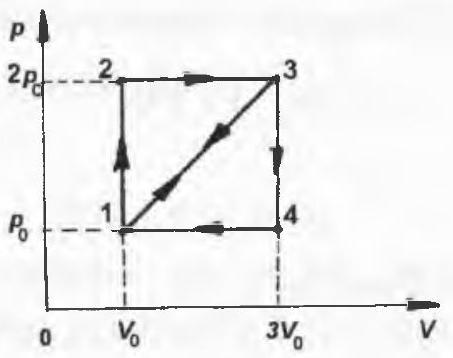
\includegraphics[max width=\textwidth, center]{2025_07_01_5b3ff9fa0d508c8e9f17g-113} Fig. 2.29\\

2.177. Un vas termoizolant este despărțit în două compartimente cu ajutorul unui perete. Într-o parte se aflǎ $\nu_{1}$ moli de oxigen $\mathrm{O}_{2}$ la temperatura $T_{1}$, iar în cealaltă parte se află $\nu_{2}$ moli de azot $\mathrm{N}_{2}$ la temperatura $T_{2}$. Temperatura stabilită în amestecul de gaze după ce peretele a fost îndepărtat este: $\left(C_{V}\left(\mathrm{O}_{2}\right)=C_{V}\left(\mathrm{~N}_{2}\right)\right)$\\ A) $\left(\nu_{1} T_{1}-\nu_{2} T_{2}\right) /\left(\nu_{1}-\nu_{2}\right)$; B) $\left(\nu_{2} T_{1}-\nu_{1} T_{2}\right) /\left(\nu_{1}-\nu_{2}\right)$; C) $\left(\nu_{1} T_{1}+\nu_{2} T_{2}\right) /\left(\nu_{1}-\nu_{2}\right)$; D) $\left(\nu_{1} T_{1}+\nu_{2} T_{2}\right) /\left(\nu_{1}+\nu_{2}\right)$; E) $\left(\nu_{2} T_{2}-\nu_{1} T_{1}\right) /\left(\nu_{1}+\nu_{2}\right)$; F) $\left(\nu_{2} T_{2}-\nu_{1} T_{1}\right) /\left(\nu_{1}-\nu_{2}\right)$.\\ (Daniela Buzatu)\\

2.178. Un gaz ideal care efectuează un ciclu Carnot cedează unui frigider $70 \%$ din căldura primită pe ciclu. Temperatura sursei calde este $T_{1}=400 \mathrm{~K}$. Temperatura frigiderului va fi:\\ A) $120 \mathrm{~K}$; B) $260 \mathrm{~K}$; C) $140 \mathrm{~K}$; D) $380 \mathrm{~K}$; E) $220 \mathrm{~K}$; F) $280 \mathrm{~K}$.\\ (Daniela Buzatu)\\

2.179. Un gaz care are coeficientul adiabatic $\gamma=1,4$ ocupă volumul $V=3 \mathrm{dm}^{3}$ şi se găseşte la presiunea $p=0,2 \mathrm{MPa}$. În urma unei încălziri izobare volumul său creşte de 3 ori. Să se calculeze cantitatea de căldură folosită la încălzire.\\ A) $3600 \mathrm{~J}$; B)$2000 \mathrm{~J}$; C) $420 \mathrm{~J}$; D) $4200 \mathrm{~J}$; E) $200 \mathrm{~J}$; F) $8400 \mathrm{~J}$.\\ (Ileana Creangă)\\

2. 180. În timpul unui proces termodinamic, un sistem primeşte o cantitate de cădură de $210 \mathrm{~kJ}$ şi în acelaşi timp sistemul se destinde la o presiune exterioară constantă de $0,8 \cdot 10^{5} \mathrm{~N} / \mathrm{m}^{2}$. Energia internă a sistemului se menține constantă în timpul procesului. Cât este variația volumului sistemului ?\\ A) $2,625 \mathrm{~m}^{3}$; B) $26 \mathrm{~m}^{3}$; C) $2,5 \mathrm{~m}^{3}$; D) $54 \mathrm{~m}^{3}$; E) $1,7 \mathrm{~m}^{3}$; F) $1,425 \mathrm{~m}^{3}$.\\ (Ileana Creangă)\\

2.181. Să se afle căldurile specifice ale unui gaz cunoscând coeficientul adiabatic $\gamma=1,4$ și densitatea gazului în condiții normale $\rho_{0}=1,293 \mathrm{~kg} / \mathrm{m}^{3}$. Se dau: $p_{0}=10^{5} \mathrm{~N} / \mathrm{m}^{2} ; T_{0}=273 \mathrm{~K}$.\\ A) $c_{V}=77,4 \mathrm{~J} / \mathrm{kg} \cdot \mathrm{K} , c_{p}=1004,36 \mathrm{~J} / \mathrm{kg} \cdot \mathrm{K}$; B) $c_{V}=174 \mathrm{~J} / \mathrm{kg} \cdot \mathrm{K} , c_{p}=369 \mathrm{~J} / \mathrm{kg} \cdot \mathrm{K}$; C) $c_{V}=717,4 \mathrm{~J} / \mathrm{kg} \cdot \mathrm{K} , c_{p}=1004,36 \mathrm{~J} / \mathrm{kg} \cdot \mathrm{K}$; D) $c_{V}=185 \mathrm{~J} / \mathrm{kg} \cdot \mathrm{K} , c_{p}=1004,36 \mathrm{~J} / \mathrm{kg} \cdot \mathrm{K}$; E) $c_{V}=217,4 \mathrm{~J} / \mathrm{kg} \cdot \mathrm{K} , c_{p}=3004,3 \mathrm{~J} / \mathrm{kg} \cdot \mathrm{K}$; F) $c_{V}=1 \mathrm{~J} / \mathrm{kg} \cdot \mathrm{K} , c_{p}=1,4 \mathrm{~J} / \mathrm{kg} \cdot \mathrm{K}$.\\ (Ileana Creangă)\\

2.182. Într-un recipient se găsesc $10 \mathrm{~kg}$ de oxigen la temperatura inițială de $27^{\circ} \mathrm{C}$. Să se afle cantitatea de căldură ce trebuie furnizată gazului într-o transformare izocoră pentru a dubla viteza pătratică medie a moleculelor gazului. Se dau: $C_{\nu}=\frac{5}{2} R ; R=8,31 \mathrm{~J} / \mathrm{mol} \cdot \mathrm{K}, \mu=32 \mathrm{~kg} / \mathrm{kmol}$.\\ A) $500 \mathrm{~kJ}$; B) $58,4 \mathrm{~kJ}$; C) $840 \mathrm{~kJ}$; D) $520 \mathrm{~kJ}$; E) $5842,9 \mathrm{~kJ}$; F) $55,8 \mathrm{~J}$.\\ (Ileana Creangă)\\

2.183. O masă $m=20 \mathrm{~g}$ de aer se dilată izobar la presiunea $p=2 \cdot 10^{5} \mathrm{~N} / \mathrm{m}^{2}$ de la o temperatură initială $t_{1}=17^{\circ} \mathrm{C}$ până la o temperatură finală $t_{2}=300^{\circ} \mathrm{C}$. Să se afle densitățile în stările (1) şi (2). Se dau: $\mu_{\text {aer }}=29 \mathrm{~kg} / \mathrm{kmol}, R=8,31 \mathrm{~J} / \mathrm{mol} \cdot \mathrm{K}$.\\ A) $\rho_{1}=2 \mathrm{~kg} / \mathrm{m}^{3}, \rho_{2}=2,2 \mathrm{~kg} / \mathrm{m}^{3}$; B) $\rho_{1}=2,40 \mathrm{~kg} / \mathrm{m}^{3}, \rho_{2}=1,26 \mathrm{~kg} / \mathrm{m}^{3}$; C) $\rho_{1}=4 \mathrm{~kg} / \mathrm{m}^{3}, \rho_{2}=12 \mathrm{~kg} / \mathrm{m}^{3}$; D) $\rho_{1}=2,40 \mathrm{~g} / \mathrm{m}^{3}, \rho_{2}=1,22 \mathrm{~g} / \mathrm{m}^{3}$; E) $\rho_{1}=3,40 \mathrm{~kg} / \mathrm{m}^{3}, \rho_{2}=7,22 \mathrm{~kg} / \mathrm{m}^{3}$; F) $\rho_{1}=0,25 \mathrm{~kg} / \mathrm{m}^{3}, \rho_{2}=1,22 \mathrm{~kg} / \mathrm{m}^{3}$.\\ (Ileana Creangă)\\

2.184. Ce masă de oxigen s-a consumat dintr-o butelie de volum $V=60$ litri dacă presiunea inițială a fost $p_{1}=10^{7} \mathrm{~N} / \mathrm{m}^{2}$ la temperatura $t_{1}=27^{\circ} \mathrm{C}$, iar presiunea finală a devenit $p=29 \cdot 10^{5} \mathrm{~N} / \mathrm{m}^{2}$ la $t_{2}=17^{\circ} \mathrm{C}$. Se dau: $\mu_{\mathrm{O}_{2}}=32 \mathrm{~kg} / \mathrm{kmol}, R=8,31 \mathrm{~J} / \mathrm{mol} \cdot \mathrm{K}$.\\ A) $5,39 \mathrm{~kg}$; B) $7,9 \mathrm{~g}$; C) $1,39 \mathrm{~kg}$; D) $3,9 \mathrm{~kg}$; E) $5,39 \mathrm{~g}$; F) $1,63 \mathrm{~kg}$.\\ (Ileana Creangă)\\

2.185. Un vas cilindric împarțit de un piston termoizolant, inițial blocat, în două volume $V_{1}=3 \mathrm{~litri}$, $V_{2}=1 \mathrm{~litru}$ conține gaz la presiunile $p_{1}=2 \cdot 10^{5} \mathrm{~N} / \mathrm{m}^{2}$, respectiv $p_{2}=10^{5} \mathrm{~N} / \mathrm{m}^{2}$ aflat la aceeaşi temperatură. Pistonul este deblocat şi gazul având volumul $V_{1}$ este încălzit până când temperatura sa absolută devine de $n=1,5$ ori mai mare decât cea inițială. Cu cât va creşte volumul $V_{1}$ ?\\ A) $0,6 \cdot 10^{-3} \mathrm{~cm}^{3}$; B) $2 \cdot 10^{-3} \mathrm{~m}^{3}$; C) $7,6 \mathrm{~m}^{3}$; D) $0,6 \cdot 10^{-3} \mathrm{~m}^{3}$; E) $6 \cdot 10^{-3} \mathrm{~m}^{3}$; F) $10^{-3} \mathrm{~m}^{3}$.\\ (Ileana Creangă)\\

2.186. O maşină termică ideală care funcționează între temperaturile $t_{1}=127^{\circ} \mathrm{C}$ şi $t_{1}=27^{\circ} \mathrm{C}$ produce un lucru mecanic de $1,5 \mathrm{kWh}$. Să se calculeze căldura primită de la sursa caldă ( $Q_{1}$ ) şi căldura cedată sursei reci( $Q_{2}$ ).\\ A) $Q_{1}=26 \mathrm{MJ}, Q_{2}=2 \mathrm{MJ}$; B) $Q_{1}=21,6 \mathrm{MJ}, Q_{2}=16,2 \mathrm{MJ}$; C) $Q_{1}=21,6 \mathrm{~J}, Q_{2}=16,2 \mathrm{~J}$; D) $Q_{1}=6 \mathrm{MJ}, Q_{2}=102 \mathrm{MJ}$; E) $Q_{1}=216 \mathrm{MJ}, Q_{2}=76,2 \mathrm{MJ}$; F) $Q_{1}=1 \mathrm{MJ}, Q_{2}=2 \mathrm{MJ}$.\\ (Ileana Creangă)\\

2.187. Să se afle masa oxigenului ( $\mu=32 \mathrm{~kg} / \mathrm{kmol}$ ) aflat într-un balon de volum $V=16,621$, la temperatura $t=27^{\circ} \mathrm{C}$ şi presiunea $p=3 \cdot 10^{6} \mathrm{~N} / \mathrm{m}^{2}$. $\left(R=8,31 \cdot 10^{3} \mathrm{~J} / \mathrm{kmolK}\right)$.\\ А) 6,4; B) $0,64 \mathrm{~kg}$; C) $0,8 \mathrm{~g}$; D) $6 \mathrm{~kg}$; E) $0,32 \mathrm{~g}$; F) $1,28 \mathrm{~kg}$.\\ (Gabriela Tiriba)\\

2.188. Într-un balon de volum $V=8,31 \mathrm{~m}^{3}$ se află heliu cu $\mu=4 \mathrm{~kg} / \mathrm{kmol} \mathrm{la}$ presiunea $p_{1}=3 \cdot 10^{5} \mathrm{~N} / \mathrm{m}^{2}$ şi temperatura $t=27^{\circ} \mathrm{C}$. În balon a mai fost introdusă o cantitate $\Delta m$ de heliu, iar presiunea a devenit $p_{2}=8 \cdot 10^{5} \mathrm{~N} / \mathrm{m}^{2}$ şi temperatura $t_{2}=47^{\circ} \mathrm{C}$. Ce masă $\Delta m$ de heliu a fost introdusă în balon? $\left(R=8,31 \cdot 10^{3} \mathrm{~J} / \mathrm{kmol} \mathrm{K}\right)$.\\ A) $6 \mathrm{~kg}$; B) $60 \mathrm{~kg}$; C) $1,2 \mathrm{~kg}$; D) $4 \mathrm{~kg}$; E) $0,4 \mathrm{~kg}$; F) $5,2 \mathrm{~kg}$.\\ (Gabriela Tiriba)\\

2.189. Căldurile specifice izobară şi respectiv izocoră ale unui gaz sunt $c_{p}=10,38 \cdot 10^{2} \mathrm{~J} / \mathrm{kgK}$ şi $c_{v}=7,41 \cdot 10^{2} \mathrm{~J} / \mathrm{kgK}$. Să se afle masa molară a gazului. ( $R=8,31 \cdot 10^{3} \mathrm{~J} / \mathrm{kmolK}$ ).\\ A) $4 \mathrm{kh} / \mathrm{kmol}$; B) $\cong 16$; C) $28 \mathrm{~kg} / \mathrm{kmol}$; D) $\cong 3 \mathrm{~kg} / \mathrm{kmol}$; E) $\cong 32 \mathrm{~kg} / \mathrm{kmol}$; F) $\cong 2 \mathrm{~kg} / \mathrm{kmol}$.\\ (Gabriela Tiriba)\\

2.190. Un gaz ocupă volumul $V_{1}=3 \mathrm{~m}^{3}$ la presiunea $p_{1}=2 \cdot 10^{5} \mathrm{~N} / \mathrm{m}^{2}$ şi temperatura $t=27^{\circ} \mathrm{C}$. Să se afle lucrul mecanic $L$ efectuat de gaz dacă acesta s-a încălzit izobar cu $\Delta T=60 \mathrm{~K}$.\\ A) $240 \mathrm{~J}$; B) $60 \mathrm{~MJ}$; C) $830 \mathrm{~J}$; D) $10 \mathrm{~kJ}$; E) $120 \mathrm{~kJ}$; F) $18 \mathrm{~MJ}$.\\ (Gabriela Tiriba)\\

2.191. O cantitate $\nu=3 \mathrm{kmol}$ de dioxid de carbon $\left(C_{p}=4 R\right)$ este încălzită izocor cu $\Delta t=50^{\circ} \mathrm{C}$. Să se afle variația energiei interne a gazului.\\ A) $250 \mathrm{~MJ}$; B) $( 120 R ) \mathrm{~kJ}$; C) $50 \mathrm{~J}$; D) $150 \mathrm{~kJ}$; E) $(900 \mathrm{R}) \mathrm{kJ}$; F) $( 450 R ) \mathrm{~J}$.\\ (Gabriela Tiriba)\\

2.192. Într-un cilindru cu piston mobil fără frecări se află o masă $m=4 \mathrm{~kg}$ de oxigen ( $\mu=32 \mathrm{~kg} / \mathrm{kmol}$ ). Ce căldură absoarbe gazul pentru ca temperatura lui să crească cu $\Delta T=16 \mathrm{~K} ?\left(C_{p}=\frac{7}{2} R\right)$\\ A) $140 \mathrm{~kJ}$; B) $20 \mathrm{~J}$; C) $(32 R) \mathrm{~J}$; D) $(7 R) \mathrm{~J}$; E) $8,3 \mathrm{~kJ}$; F) $490 \mathrm{~kJ}$.\\ (Gabriela Tiriba)\\

2.193. Un motor ideal ce functionează după un ciclu Carnot, absoarbe căldura $Q_{1}=9 \cdot 10^{4} \mathrm{~J}$ de la sursa caldă. Să se afle căldura $Q_{2}$ cedată sursei reci dacă temperatura sursei calde este $T_{1}=450 \mathrm{~K}$, iar temperatura sursei reci este $T_{1}=350 \mathrm{~K}$.\\ A) $70 \mathrm{~kJ}$; B) $45 \cdot 10^{4} \mathrm{~J}$; C) $35 \mathrm{~kJ}$; D) $140 \mathrm{~J}$; E) $90 \mathrm{~kJ}$; F) $300 \mathrm{~kJ}$.\\ (Gabriela Tiriba)\\

2.194. Să se determine masa unui obiect de zinc ştiind că acesta are o capacitate calorică măsurată $C=0,7 \mathrm{~kJ} / \mathrm{K}$. Se dă $c_{\mathrm{Zn}}=400 \mathrm{~J} / \mathrm{kgK}$.\\ A) $2,1 \mathrm{~kg}$; B) $1,75 \mathrm{~kg}$; C) $280 \mathrm{~g}$; D) $0,57 \mathrm{~kg}$; E) $1,75 \mathrm{~g}$; F) $0,75 \mathrm{~kg}$.\\ (Liliana Preda)\\

2.195. O cantitate de $\nu=0,4 \mathrm{~moli}$ de gaz ideal, biatomic aflată într-o stare caracterizată de $V_{1}=5$ litri şi $t_{1}=27^{\circ} \mathrm{C}$ este încălzită izobar până în starea cu $T_{2}=1,5 T_{1}$. Să se calculeze lucrul mecanic efectuat de gaz în cursul procesului de încălzire.\\ A) $995 \mathrm{~J}$; B) $663 \mathrm{~J}$; C) $2 \mathrm{~kJ}$; D) $498,6 \mathrm{~J}$; E) $1,492 \mathrm{~J}$; F) $2,98 \mathrm{~kJ}$.\\ (Liliana Preda)\\

2.196. O masă $m=44,8 \mathrm{~kg}$ de azot considerat gaz biatomic este supus unui proces de încălzire caracterizat prin $Q=\Delta U=3,324 \mathrm{MJ}$. Să se determine cu cât a crescut temperatura gazului în urma procesului de încălzire. Se dau: $\mu_{\text {azot }}=28 \mathrm{~kg} / \mathrm{kmol}, C_{v}=\frac{5}{2} R$.\\ A) $15 \mathrm{~K}$; В) $10^{\circ} \mathrm{C}$; C) $256^{\circ} \mathrm{C}$; D) $70 \mathrm{~K}$; E) $0^{\circ} \mathrm{C}$; F) $100 \mathrm{~K}$.\\ (Liliana Preda)\\

2.197. Să se determine viteza termică a moleculelor de azot aflate la presiunea $p=2 \cdot 10^{3} \mathrm{~N} / \mathrm{m}^{2}$ într-o incintă de volum $V=6$ litri şi conținând $0,1 \mathrm{~g}$ de substanță.\\ A) $12 \mathrm{~m} / \mathrm{s}$; B) $6 \mathrm{~m} / \mathrm{s}$; C) $979 \mathrm{~m} / \mathrm{s}$; D) $0,6 \mathrm{~m} / \mathrm{s}$; E) $600 \mathrm{~m} / \mathrm{s}$; F) $21,6 \mathrm{~km} / \mathrm{h}$.\\ (Liliana Preda)\\

2.198. Să se determine densitatea gazului aflat într-o incintă la presiunea $p=1 \mathrm{~atm}$, dacă viteza termică a moleculelor acestuia este $v_{T}=550 \mathrm{~m} / \mathrm{s}$.\\ A) $0,33 \mathrm{~kg} / \mathrm{m}^{3}$; B) $5,52 \cdot 10^{-3} \mathrm{~kg} / \mathrm{m}^{3}$; C) $1 \mathrm{~g} / \mathrm{cm}^{3}$; D) $1 \mathrm{~kg} / \mathrm{m}^{3}$; E) $3,3 \cdot 10^{-3} \mathrm{~g} / \mathrm{m}^{3}$; F) $5,52 \mathrm{~kg} / \mathrm{m}^{3}$.\\ (Liliana Preda)\\

2.199. Într-un pahar de $15 \mathrm{~cm}$ înălțime umplut două treimi cu apă se introduce vertical, până la fund, un pai având o lungime $l=20 \mathrm{~cm}$ și un diametru $d=4 \mathrm{~mm}$. Care trebuie să fie forța minimă de aspirație inițială aplicată la capătul liber al paiului pentru a scoate apa din pahar. Se dă presiunea atmosferei înconjurătoare $p_{0}=1,013 \cdot 10^{5} \mathrm{~N} / \mathrm{m}^{2}$.\\ A) $1,28 \mathrm{~N}$; B) $10 \mathrm{~N}$; C) $1,3 \mathrm{~N}$; D) $1,27 \mathrm{~N}$; E) $2 \mathrm{~N}$; F) $7 \mathrm{~N}$.\\ (Liliana Preda)\\

2.200. Un vas de volum $V_{1}=20 \mathrm{~litri}$ care contine gaz la temperatura $t_{1}=27^{\circ} \mathrm{C}$ şi presiune normală, este legat printr-un tub scurt cu alt vas de volum $V_{2}=5$ litri, vidat. Tubul de legătură este prevăzut cu un robinet care permite trecerea gazului dintr-un vas în altul. Să se calculeze fracțiunea din masa totală de gaz care trece dintr-un vas în altul la încălzirea acestora cu $200^{\circ} \mathrm{C}$.\\ А) 0,5; B) $20 \%$; C) 0,4; D) $30 \%$; E) 1,2; F) $70 \%$.\\ (Liliana Preda)\\

2.201. O cantitate de $0,1 \mathrm{kmoli}$ de gaz ideal trece din starea (1) în starea (2) printr-o transformare ca cea din Fig. 2.30. Sã se determine presiunea gazului în starea (2), ştiind că, în starea (1), gazul ocupă volumul $V_{1}=2 \mathrm{~m}^{3}$ la temperatura ${t}_{1}=127^{\circ} \mathrm{C}$. Se dă : $R=8310 \mathrm{~J} / \mathrm{kmolK}$.\\ A) $3,2 \mathrm{~atm}$; B) $1,66 \cdot 10^{5} \mathrm{~N} / \mathrm{m}^{2}$; C) $0,5 \cdot 10^{5} \mathrm{~N} / \mathrm{m}^{2}$; D) $2,45 \cdot 10^{5} \mathrm{~N} / \mathrm{m}^{2}$; E) $3,21 \cdot 10^{5} \mathrm{~N} / \mathrm{m}^{2}$; F) $0,51 \mathrm{~atm}$.\\ (Liliana Preda)\\ 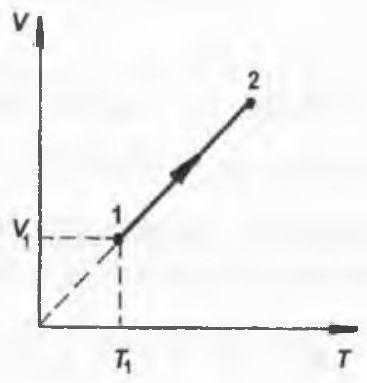
\includegraphics[max width=\textwidth, center]{2025_07_01_5b3ff9fa0d508c8e9f17g-119} Fig. 2.30\\

2.202. Un boiler având o capacitate de $10 \mathrm{~liltri}$ este proiectată astfel încât să încălzească volumul maxim de apă de la temperatura $t_{1}=15^{\circ} \mathrm{C}$ la $t_{2}=75^{\circ} \mathrm{C}$ în $20 \mathrm{~min}$. Să se calculeze valoare rezistenţei folosite ca element de incălzire ştiind că boilerul este alimentat de la o sursă normală de $220 \mathrm{~V}$. Se cunosc $c_{a p a}=4180 \mathrm{~J} / \mathrm{kgK} ; \rho_{a p a}=1000 \mathrm{~kg} / \mathrm{m}^{3}$.\\ А) $23,15 \Omega$; B) $1,1 \Omega$; C) $0,95 \Omega$; D) $23,15 \mathrm{k} \Omega$; E) $385 \Omega$; F) $11,57 \Omega$.\\ (Liliana Preda)\\

2.203. Un vehicul cu masa $M=500 \mathrm{~kg}$ este deplasat cu ajutorul unui motor având un randament de $60 \%$ din randamentul unei maşini Carnot funcționând între temperaturile $t_{1}=327^{\circ} \mathrm{C}$ şi $t_{2}=27^{\circ} \mathrm{C}$. Să se calculeze ce cantitate de combustibil cu puterea calorică $q=4,18 \cdot 10^{7} \mathrm{~J} / \mathrm{kg}$ consumă motorul pentru a străbate cu viteză constantă de $54 \mathrm{~km} / \mathrm{h}$ o distanță de 3 km pe o pantă cu unghiul de înclinare $\alpha=30^{\circ}$. Se dă coeficientul de frecare pe pantă $\mu=0,1$.\\ A) $1 \mathrm{~kg}$; B) $117 \mathrm{~g}$; C) $0,68 \mathrm{~kg}$; D) $0,1 \mathrm{~kg}$; E) $400 \mathrm{~g}$; F) $0,34 \mathrm{~kg}$.\\ (Liliana Preda)\\

2.204. Un kilomol de oxigen este închis într-un cilindru cu piston mobil. Gazul suferă o comprimare până la o treime din volumul inițial. Simultan, el se încălzeşte ca urmare a acceptării unei energii din exterior, până la o temperatură de patru ori mai mare. De câte ori creşte presiunea gazului?\\ A) 7 ori; B) 3 ori; C) $3 / 4 \mathrm{ori}$; D) $3 / 4 \mathrm{ori}$; E) 12 ori; F) 0,5 ori.\\ (Cristina Stan)\\

2.205. Un gaz ideal monoatomic se află inițial la temperatura camerei. Gazul se destinde izobar până la un volum de şapte ori mai mare. Cât este raportul dintre lucrul mecanic efectuat de gaz şi căldura primită? Se cunoaşte $C_{p}=5 / 2 R$.\\ A) $\frac{2}{5}$; B) $\frac{5}{2}$; C) 5; D) 7; E) $\frac{1}{7}$; F) 8.\\ (Cristina Stan)\\

2.206. O maşină termică ideală care functionează după un ciclu Carnot, primeşte de la o sursă caldă, de temperatură $327^{\circ} \mathrm{C}$, energia $10^{6} \mathrm{~J}$. Temperatura sursei reci cu care este în contact mașina termică este de $27^{\circ} \mathrm{C}$. Cât ester lucrul mecanic efectuat de sistem ?\\ A) $5 \cdot 10^{3} \mathrm{~J}$; B) $5 \cdot 10^{5} \mathrm{~J}$; C) $9,2 \cdot 10^{5} \mathrm{~J}$; D) $8,9 \cdot 10^{3} \mathrm{~J}$; E) $10^{5} \mathrm{~J}$; F) $1,09 \cdot 10^{5} \mathrm{~J}$.\\ (Cristina Stan)\\

2.207. Un corp din material plastic este încălzit până la $100^{\circ} \mathrm{C}$ şi apoi este cufundat într-un vas izolat termic, ce conține o masă dublă de apă la temperatura $20^{\circ} \mathrm{C}$. După un timp se stabileşte echilibrul termic la temperatura $40^{\circ} \mathrm{C}$. De câte ori este mai mare căldura specifică a apei decât cea a plasticului?\\ A) $\frac{1}{3}$; B) 3; C) $\frac{3}{2}$; D) sunt egale; E) $\frac{2}{3}$; F) 5.\\ (Cristina Stan)\\

2.208. Un sistem închis absoarbe căldura $20 \mathrm{~MJ}$ şi efectuează un lucru mecanic de $7 \mathrm{~MJ}$. Procesul este inversat şi sistemul ajunge din nou în starea inițială, cedând energia $25 \mathrm{~MJ}$ sub formă de căldură. Care este variația totală de energie internă a sistemului?\\ A) $-12 \mathrm{~MJ}$; B) $12 \mathrm{~MJ}$; C) $13 \mathrm{~MJ}$; D) $38 \mathrm{~MJ}$; E) 0; F) $-13 \mathrm{~MJ}$.\\ (Cristina Stan)\\

2.209. Folosiți ciclul reprezentat în Fig. 2.31 pentru a alege afirmațiile corecte dintre următoarele variante: 1. presiunea în A este $2,4 \cdot 10^{5} \mathrm{~N} / \mathrm{m}^{2}$; 2. temperatura în C este de trei ori mai mică decât în D ; 3. temperatura în $B$ creşte de 4,8 ori față de cea din $D$; 4. sistemul nu primeşte căldură pe ramura AB .\\ A) 1 şi 2; B) 1,2 şi 4; C) 1 şi 3; D) 1,2 şi 3; E) toate; F) 1.\\ (Cristina Stan)\\ 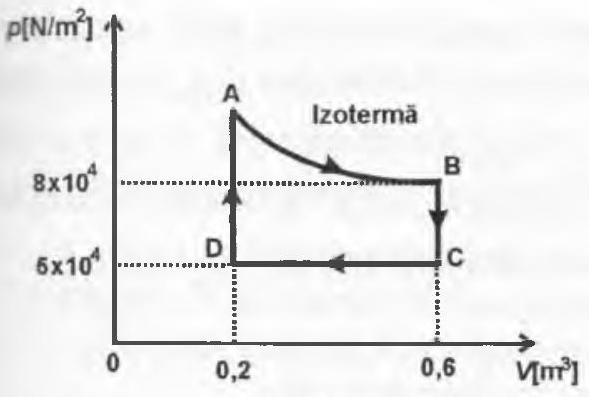
\includegraphics[max width=\textwidth, center]{2025_07_01_5b3ff9fa0d508c8e9f17g-121} Fig. 2.31\\

2.210. Folosind diagrama din Fig. 2.32 analizați câte dintre afirmațiile următoare sunt adevărate: 1. lucrul mecanic este zero pe ramura BC ; 2. temperatura în A este de 5 ori mai mică decât cea din C ; 3. temperatura în B este egală cu cea din C ; 4. lucrul mecanic efectuat pe întreg ciclul este egal cu căldura primită.\\ A) 1; B) 2; C) toate; D) 3; E) nici una; F) 4.\\ (Cristina Stan)\\ 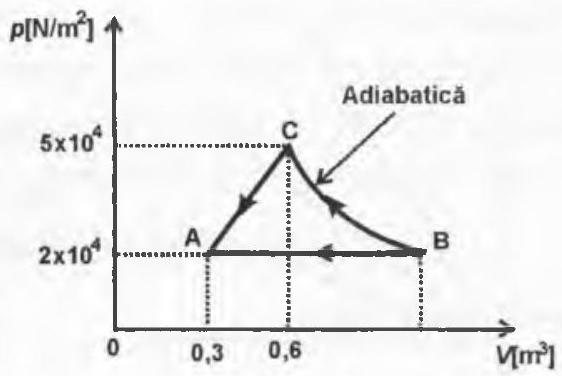
\includegraphics[max width=\textwidth, center]{2025_07_01_5b3ff9fa0d508c8e9f17g-121(1)} Fig. 2.32\\

2.211. Legea transformării izocore a gazului ideal are expresia:\\ A) $\frac{\Delta p}{p_{0}}=\frac{t}{T}$; B) $\frac{p}{p_{0}}=1+\beta t$; C) $\frac{\Delta p}{\Delta t}=\alpha$; D) $\frac{p}{p_{0}}=\beta t$; E) $\frac{\Delta p}{T}=$ const.; F) $p T=$ const.\\ (Nicoleta Eşeanu)\\

% Nu stiu daca putem avea "." in interiorul variantelor de raspuns care nu sunt F)
2.212. Legea transformării izobare a gazului ideal are expresia:\\ A) $\frac{\Delta V}{V_{0}}=\alpha t$; B) $\frac{\Delta p}{p_{0}}=\beta t$; C) $\frac{V}{V_{0}}=\alpha t$; D) $\frac{\Delta V}{T}=$ const.; E) $\frac{V}{T_{0}}=$ const.; F) $\frac{\Delta V}{\Delta t}=\alpha$.\\ (Nicoleta Eşeanu)\\

2.213. Care din mărimile următoare are aceeaşi unitate de măsură ca şi constanta Boltzmann?\\ A) căldura molară; B) căldura specifică; C) energia internă; D) capacitatea calorică; E) căldura latentă specifică de topire; F) constanta universală a gazelor ideale.\\ (Nicoleta Eşeanu)\\

2.214. Dreptele din Fig. 2.33 sunt trasate pentru mase egale de hidrogen ( $\mu_{\mathrm{H}_{2}}=2 \mathrm{~kg} / \mathrm{kmol}$ ), metan $\left(\mu_{\mathrm{CH}_{4}}=16 \mathrm{~kg} / \mathrm{kmol}\right)$ şi heliu ( $\mu_{\mathrm{He}}=4 \mathrm{~kg} / \mathrm{kmol}$ ), aflate în butelii identice. Care dreaptă corespunde metanului?\\ A) dreapta 1; B) dreapta 2; C) dreapta 3; D) dreptele 1 şi 2; E) dreptele 2 şi 3; F) nu se poate determina.\\ (Nicoleta Eşeanu)\\ 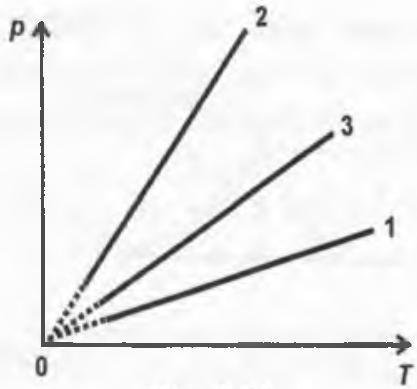
\includegraphics[max width=\textwidth, center]{2025_07_01_5b3ff9fa0d508c8e9f17g-122} Fig. 2.33\\

2.215. Două mase de gaz ideal, având aceeaşi căldură molară la volum constant, se află în două vase unite printr-un tub de volum neglijabil, închis inițial de un robinet. Sistemul are un înveliş adiabatic. Parametrii de stare sunt ( $p, 2 V, T$ ) şi, respectiv ( $2 p / 3, V, 2 T / 3$ ). Deschidem robinetul şi sistemul ajunge la echilibru termodinamic. Temperatura finală este:\\ A) $8 T / 9$; B) $3 T / 7$; C) $7 T / 9$; D) $8 T / 21$; E) $7 T / 3$; F) $5 T / 3$.\\ (Nicoleta Eşeanu)\\

2.216. O masă de gaz ideal descrie ciclul termic din Fig. 2.34, în care transformarea $2 \rightarrow 1$ este izotermă. Să se calculeze lucrul mecanic efectuat de gaz în acest ciclu ( $\ln 2 \approx 0,7$ ).\\ A) $1,45 p_{1} V_{1}$; B) $\frac{p_{1} V_{1}}{2}$; C) $\frac{p_{1} V_{1}}{20}$; D) $0,8 p_{1} V_{1}$; E) $0,45 p_{1} V_{1}$; F) $0,5 p_{1} V_{1}$.\\ (Nicoleta Eşeanu)\\ 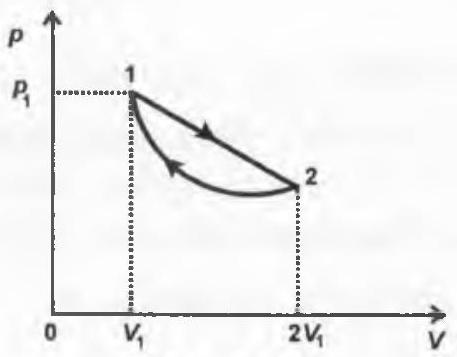
\includegraphics[max width=\textwidth, center]{2025_07_01_5b3ff9fa0d508c8e9f17g-122(1)} Fig. 2.34\\

2.217. Un recipient de volum $V=2 \mathrm{dm}^{3}$ conține gaz ideal la temperatura $t_{1}=27^{\circ} \mathrm{C}$. Încălzim sistemul la $t_{2}=87^{\circ} \mathrm{C}$. Prin supapa de siguranţă, care asigură menținerea unei presiuni constante $p_{0}$ (presiunea atmosferică normală, $760 \mathrm{~tori}$), iese afară o masă $\Delta m=3 \mathrm{~g}$ de gaz. Calculați din aceste date densitatea gazului în condiții normale de presiune și temperatură $\left(\rho_{0}\right)$ ).\\ A) $1,5 \mathrm{~g} / \mathrm{dm}^{3}$; B) $3,85 \mathrm{~g} / \mathrm{dm}^{3}$; C) $8,5 \mathrm{~g} / \mathrm{dm}^{3}$; D) $9,89 \mathrm{~g} / \mathrm{dm}^{3}$; E) $15,2 \mathrm{~g} / \mathrm{dm}^{3}$; F) nici o variantă nu este corectă.\\ (Nicoleta Eşeanu)\\

2.218. Două recipiente de volume $V_{1}$ și $V_{2}=5 V_{1}$, termostatate la temperaturile $T_{1}$, respectiv $T_{2}=7 T_{1} / 6$, conțin gaze ideale la presiunile $p_{1}$, respectiv $p_{2}=2 p_{1}$. Recipientele sunt legate printr-un tub de volum neglijabil, inchis inițial cu un robinet. După deschiderea robinetului presiunea gazului este:\\ A) $0,72 p_{1}$; B) $0,9 p_{1}$; C) $1,8 p_{1}$; D) $2,5 p_{1}$; E) $3,2 p_{1}$; F) $5,6 p_{1}$.\\ (Nicoleta Eşeanu)\\

2.219. Într-un cilindru vertical închis, vidat, cu lungimea $l=30 \mathrm{~cm}$, este suspendat printr-un resort un piston de masă neglijabilă care se poate deplasa etanş, fără frecări. Inițial, pistonul este în echilibru pe fundul vasului. Sub piston se introduce o cantitate de aer astfel încât pistonul se ridică cu $h_{1}=10 \mathrm{~cm}$, temperatura sistemului find $t_{1}=27^{\circ} \mathrm{C}$. Micşorăm cantitatea de aer de patru ori şi modificăm temperatura astfel încât pistonul se află acum la $h_{2}=6 \mathrm{~cm}$. Temperatura finalǎ este:\\ A) $44,7^{\circ} \mathrm{C}$; B) $75^{\circ} \mathrm{C}$; C) $270 \mathrm{~K}$; D) $389 \mathrm{~K}$; E) $159^{\circ} \mathrm{C}$; F) $175^{\circ} \mathrm{C}$.\\ (Nicoleta Eşeanu)\\

2.220. Un ciclu Carnot funcționează între temperaturile $t_{1}=127^{\circ} \mathrm{C}$ şi $t_{2}=27^{\circ} \mathrm{C}$. Dacă micșorăm temperatura minimă cu $50^{\circ} \mathrm{C}$ obținem un randament $\eta_{1}$, iar dacă mărim temperatura maximă cu $50^{\circ} \mathrm{C}$ obținem un randament $\eta_{2}$. Raportul $\eta_{1} / \eta_{2}$ este:\\ А) 1,8; B) $4 / 9$; C) 9/8; D) 1; E) 1,25; F) 2,6.\\ (Nicoleta Eşeanu)\\

2.221. Într-un vas de capacitate calorică $C_{\text {vas }}=500 \mathrm{~J} / \mathrm{K}$ se află $m_{a}=500 \mathrm{~g}$ apă având căldura specifică $c_{1}=4180 \mathrm{~J} / \mathrm{kg} \cdot \mathrm{K}$, la temperatura $t_{1}=20^{\circ} \mathrm{C}$. Se introduce o bilă de cupru de masă $m_{2}=200 \mathrm{~g}$ şi căldură specifică $c_{2}=400 \mathrm{~J} / \mathrm{kg} \cdot \mathrm{K}$, încălzită la $t_{2}=120^{\circ} \mathrm{C}$. Temperatura de echilibru este:\\ A) $24,8^{\circ} \mathrm{C}$; B) $23,7^{\circ} \mathrm{C}$; C) $22,4^{\circ} \mathrm{C}$; D) $23^{\circ} \mathrm{C}$; E) $44,8^{\circ} \mathrm{C}$; F) $52,5^{\circ} \mathrm{C}$.\\ (Nicoleta Eşeanu)\\

2.222. Energia internă a unei mase $m=10 \mathrm{~g}$ de gaz ideal monoatomic aflat la presiunea $p=100 \mathrm{kPa}$, având densitatea $\rho=0,8 \mathrm{~kg} / \mathrm{m}^{3}$, este:\\ A) $150 \mathrm{~J}$; B) $1,25 \mathrm{~kJ}$; C) $1875 \mathrm{~J}$; D) $625 \mathrm{~J}$; E) $875 \mathrm{~J}$; F) nici o variantă din cele prezentate nu este corectă.\\ (Nicoleta Eşeanu)\\

2.223. O masă de oxigen ( $C_{V}=5 R / 2$ ), aflată la presiunea $p_{1}=3 \cdot 10^{5} \mathrm{~N} / \mathrm{m}^{2}$ şi volumul $V_{1}=6$ litri, suferă o transformare izobară în care $V_{2}=4 V_{1}$, urmată de una izocoră pânǎ la presiunea $p_{3}=p_{2} / 1,5$. Variaţia totală a energiei interne a gazului este:\\ A) $7,5 \mathrm{~kJ}$; B) $180 \mathrm{~J}$; C) $20 \mathrm{~J}$; D) $1,2 \mathrm{~kJ}$; E) $2,4 \mathrm{~kJ}$; F) nici o variantă nu este corectă.\\ (Nicoleta Eşeanu)\\

2.224.* Un kilomol de neon ( $\mu=20 \mathrm{~kg} / \mathrm{kmol}$ ) descrie o transformare ciclică formată din două izobare şi două izocore. Se cunosc: $p_{1}=100 \mathrm{kPa}, V_{1}=4 \mathrm{~m}^{3}$, $V_{2}=3 V_{1}$ și $T_{1}=T_{3}$. Să se calculeze raportul vitezelor termice extreme ale moleculelor gazului pentru acest ciclu.\\ A) 2; B) $2 \sqrt{2}$; C) 3; D) $3 \sqrt{2}$; E) 4; F) $4 \sqrt{3}$.\\ (Nicoleta Eşeanu)\\

2.225. Un corp mic, sferic, confecţionat din oțel, cade liber în câmpul gravitațional al Pământului. El atinge o suprafață dură, aşezată pe sol, cu viteza $v=40 \mathrm{~m} / \mathrm{s}$ şi, după ciocnirea cu aceasta, se ridică la înălțimea $h=4 \mathrm{~m}$. Se presupune că întreaga căldură degajată prin ciocnire este preluată de corp. Cu cât creşte temperatura corpului ? Se cunosc $c=400 \mathrm{~J} / \mathrm{kg} \cdot \mathrm{K}$ şi $g \cong 10 \mathrm{~m} / \mathrm{s}^{2}$.\\ A) $275 \mathrm{~K}$; B) $18 \mathrm{~K}$; C) $28,9 \mathrm{~K}$; D) $8,6 \mathrm{~K}$; E) $1,9^{\circ} \mathrm{C}$; F) $4,3^{\circ} \mathrm{C}$.\\ (Nicoleta Eşeanu)\\

2.226. În Sistemul Internațional de unități de măsură (S.I.) numărul lui Avogadro se exprimă în:\\ A) molecule pe mol; B) molecule pe metru cub; C) kilomol pe metru cub; D) molecule pe kilomol; E) molecule; F) este adimensional.\\ (Constantin Neguțu)\\

2.227. Într-o incintă se află în amestec aer ( $\mu_{1}=28,9 \mathrm{~kg} / \mathrm{kmol}$ ) şi vapori saturanți de apă ( $\mu_{2}=18 \mathrm{~kg} / \mathrm{kmol}$ ). Raportul dintre viteza termică a moleculelor de aer şi cea a moleculelor de apă este:\\ А) 1; B) 2,35; C) 1,27; D) 0,63; E) 1,94; F) 0,79.\\ (Constantin Neguțu)\\

2.228. Un gaz ideal se destinde după legea $p^{2} \cdot V=$ const. În acest proces:\\ A) $p$ şi $T$ cresc; B) $p$ creşte şi $T$ scade; C) $p$ scade şi $T$ creşte; D) $p$ şi $T$ scad; E) $p$ scade şi $T$ rămâne constantă; F) numărul de moli de gaz scade la jumătate.\\ (Constantin Neguțu)\\

2.229. Un cilindru orizontal este împărțit în patru compartimente egale prin intermediul a trei pistoane identice aflate in echilibru mecanic. Notăm cu $p$ presiunea gazelor din cele patru compartimente în această stare. Dacă se aşază cilindrul vertical, echilibrul corespunde volumelor $V_{2}=2 V_{1} ; V_{3}=3 V_{1} ; V_{4}=4 V_{1}$. Presiunea gazului din compartimentul inferior (de volum $V_{1}$ ) este:\\ A) $\frac{5}{2} p$; B) $\frac{3}{2} p$; C) $\frac{5}{4} p$; D) $\frac{15}{2} p$; E) $5 p$; F) $2 p$.\\ (Constantin Neguțu)\\

2.230. Un motor cu reacție funcționează după un ciclu reversibil format din două adiabate şi două izobare, ca în Fig. 2.35. Randamentul ciclului, în funcție de exponentul adiabatic al gazului de lucru, $\gamma$, şi de raportul $p_{2} / p_{1}=\rho$, este:\\ A) $1-\frac{1}{\rho^{\gamma-1}}$; В) $1-\frac{1}{\rho^{\gamma}}$; C) $1-\frac{\rho^{\gamma}-1}{\rho-1}$; D) $1-\frac{\rho^{\gamma}}{\rho-1}$; Е) $1-\left(\frac{1}{\rho}\right)^{\frac{\gamma-1}{\gamma}}$; F) $1-\frac{\rho}{\rho-1}$.\\ (Constantin Neguțu)\\ 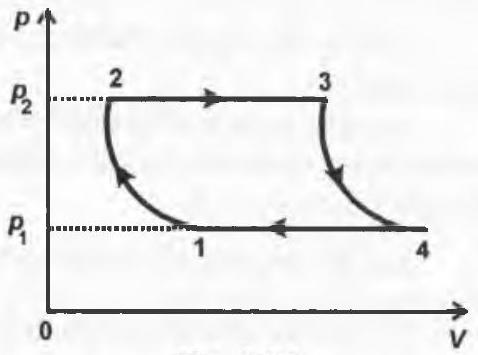
\includegraphics[max width=\textwidth, center]{2025_07_01_5b3ff9fa0d508c8e9f17g-125} Fig. 2.35\\

2.231. O cantitate de azot cu masa $m=1,4 \mathrm{~kg}$, aflată la temperatura $T_{1}=362 \mathrm{~K}$, se destinde adiabatic efectuând lucrul mecanic $L=8,31 \mathrm{~kJ}$. Cunoscând constanta gazelor perfecte, $R=8310 \mathrm{~J} / \mathrm{kmol} \cdot \mathrm{K}$, şi masa molară a azotului, $\mu_{\mathrm{N}_{2}}=28 \mathrm{~kg} / \mathrm{kmol}$, temperatura finală a gazului este:\\ A) $370 \mathrm{~K}$; B) $354 \mathrm{~K}$; C) $348 \mathrm{~K}$; D) $352 \mathrm{~K}$; E) $374 \mathrm{~K}$; F) $373 \mathrm{~K}$.\\ (Constantin Neguțu)\\

2.232. Într-un cilindru orizontal umplut cu gaz se află un piston mobil care imparte cilindrul în raportul lungimilor $l_{2} / l_{1}=2$ (Fig. 2.36). Cât va deveni acest raport dacă primul compartiment este încălzit până la temperatura $\theta_{1}=27^{\circ} \mathrm{C}$, iar al doilea răcit până la temperatura $\theta_{2}=-123^{\circ} \mathrm{C}$ ?\\ А) 1,5; B) 2; C) 1; D) 0,5; E) 2,5; F) 3.\\ (Constantin Neguțu)\\ 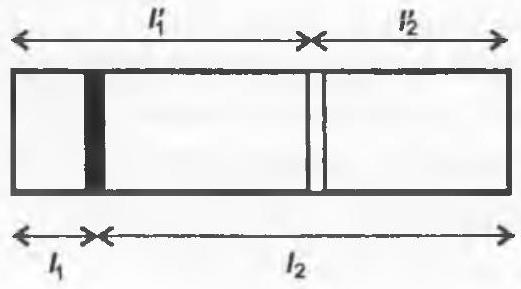
\includegraphics[max width=\textwidth, center]{2025_07_01_5b3ff9fa0d508c8e9f17g-126(1)} Fig. 2.36\\

2.233. În timpul transformării prezentate în Fig. 2.37, presiunea unei mase de gaz ideal:\\ A) creşte; B) rămâne constantă; C) nu se poate specifica nimic în legătură cu variația presiunii; D) scade; E) tinde la zero; F) tinde asimptotic la o valoare bine precizata.\\ (Constantin Negutu)\\ 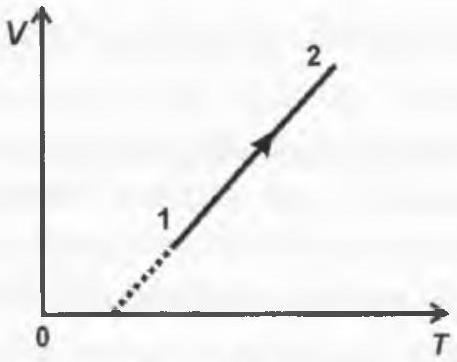
\includegraphics[max width=\textwidth, center]{2025_07_01_5b3ff9fa0d508c8e9f17g-126} Fig. 2.37\\

2.234. Alegeți afirmația adevărată:\\ A) lucrul mecanic efectuat de un gaz ideal nu depinde decât de stările inițială și finală ale sistemului; B) căldura schimbată de un sistem termodinamic este o funcție de stare; C) variația energiei interne a unui sistem termodinamic este o mărime de proces; D) în comprimarea izotermă a unui gaz ideal, cǎldura cedată este numeric egală cu variația energiei interne; E) lucrul mecanic efectuat de un gaz ideal biatomic într-o destindere izobară este de 2,5 ori mai mare decât variația energiei interne în acelaşi proces; F) pentru încălzirea izobară a unui gaz ideal este necesară mai multă căldură decât pentru încălzirea izocoră cu acelaşi număr de grade.\\ (Constantin Neguțu)\\

2.235. Alegeți afirmația adevărată:\\ A) comprimarea adiabatică a gazului într-un cilindru cu piston presupune deplasarea lentă a pistonului; B) dacă un gaz este comprimat lent, el suferă o transformare izocoră; C) la încălzirea adiabatică a unui gaz, presiunea sa scade; D) densitatea unui gaz creşte prin încălzire izobară; E) presiunea unui gaz comprimat după legea $T=a V^{2}$, unde $a$ este o constantă, scade; F) în aceleaşi condiții de temperatură şi presiune, două gaze cu mase molare diferite au volume molare diferite.\\ (Constantin Neguțu)\\

2.236. Concentrația moleculelor unui gaz ideal:\\ A) este aceeaşi indiferent de presiunea şi temperatura lui; B) creşte prin încălzirea gazului la presiune constantă; C) scade prin destindere izotermă; D) la aceeași densitate, este mai mică pentru un gaz cu masa molară mai mică; E) scade cu creşterea izotermă a presiunii; F) creşte cu creşterea volumului.\\ (Constantin Negutu)\\

2.237. Un volum de $2 \mathrm{~litri}$ de aer, aflat inițial în condiții normale de temperatură și presiune, se încălzeşte izobar absorbind o cantitate de căldură $Q=709,3 \mathrm{~J}$. Volumul gazului:\\ A) creşte de 3 ori; B) creşte de 2 ori; C) scade de două ori; D) scade de 3 ori; E) creşte de 4 ori; F) scade de 4 ori.\\ (Constantin Neguțu)\\

2.238. Un cuptor este încălzit de la $27^{\circ} \mathrm{C}$ la $1727^{\circ} \mathrm{C}$. Procentul din masa de aer care iese din cuptor în acest timp este:\\ A) $50 \%$; B) 0; C) $10 \%$; D) $85 \%$; E) $90 \%$; F) $30 \%$.\\ (Constantin Negutu)\\

2.239. O masă $m=10 \mathrm{~g}$ de azot suferă o transformare în care presiunea scade liniar cu volumul din starea cu $p_{1}=1 \mathrm{~atm}, V_{1}=8 \mathrm{~litri}$, în starea cu $p_{2}=3 \mathrm{~atm}$, $V_{2}=4 \mathrm{~litri}$. Temperatura maximă atinsă de gaz în decursul acestei transformări este:\\ A) $421 \mathrm{~K}$; В) $450 \mathrm{~K}$; C) $145^{\circ} \mathrm{C}$; D) $430 \mathrm{~K}$; E) $254^{\circ} \mathrm{C}$; F) $400 \mathrm{~K}$.\\ (Constantin Neguțu)\\

2.240. Un recipient ce conține $0,1 \mathrm{~kmoli}$ de heliu (cu masa molară $\mu=4 \mathrm{~kg} / \mathrm{kmol}$ ) la volumul $V_{1}=0,83 \mathrm{~lm}^{3}$ şi presiunea $p_{1}=10^{5} \mathrm{~N} / \mathrm{m}^{2}$ este pus în contact cu un recipient ce conține $0,1 \mathrm{kmoli}$ de heliu, având volumul $V_{2}=1,662 \mathrm{~m}^{3}$ şi presiunea $p_{2}=3 \cdot 10^{5} \mathrm{~N} / \mathrm{m}^{2}$. Să se afle valoarea finală a temperaturii după ce între cele două recipiente se stabileşte o legătură.\\ А) $350 \mathrm{~K}$; В) $250 \mathrm{~K}$; C) $150 \mathrm{~K}$; D) $351^{\circ} \mathrm{C}$; E) $400 \mathrm{~K}$; F) $450 \mathrm{~K}$.\\ (Cristian Toma)\\

2.241. Într-un balon de volum $V=0,623 \mathrm{~m}^{3}$ se află heliu la presiunea $p_{1}=10^{5} \mathrm{~N} / \mathrm{m}^{2}$ şi temperatura de $27^{\circ} \mathrm{C}$ (masa molară a heliului fiind $\mu=4 \mathrm{~kg} / \mathrm{kmol}$ ). După ce se mai introduce heliu (în condiții de temperatură şi volum constante) presiunea ajunge la $p_{2}=2 \cdot 10^{5} \mathrm{~N} / \mathrm{m}^{2}$. Ce cantitate de heliu s-a introdus?\\ A) $1 \mathrm{~kg}$; B) $0,01 \mathrm{~kg}$; C) $0,1 \mathrm{~kg}$; D) $10 \mathrm{~kg}$; E) $10 \mathrm{~g}$; F) $2,5 \mathrm{~kg}$.\\ (Cristian Toma)\\

2.242.* Un gaz aflat la o anumită presiune $p_{1}$ are viteza termică $v_{t_{1}}=10 \mathrm{~m} / \mathrm{s}$. Să se indice viteza termică a aceluiaşi gaz dacă presiunea creşte de 100 ori, în condiții de volum constant.\\ A) $1000 \mathrm{~m} / \mathrm{s}$; B) $0,1 \mathrm{~m} / \mathrm{s}$; C) $50 \mathrm{~m} / \mathrm{s}$; D) $100 \mathrm{~m} / \mathrm{s}$; E) $20 \mathrm{~m} / \mathrm{s}$; F) $10 \mathrm{~m} / \mathrm{s}$.\\ (Cristian Toma)\\

2.243. Un recipient ce conține vapori de apă la temperatura de $497 \mathrm{~K}$, volumul $V=3,1 \mathrm{~m}^{3}$ şi presiunea atmosferică $p=10^{5} \mathrm{~N} / \mathrm{m}^{2}$, începe să primească alți vapori de apă printr-un orificiu, fiind menținute în permanență valorile inițiale ale presiunii şi volumului. Să se indice câți moli poate primi recipientul, pentru ca moleculele de apă să ocupe în continuare întregul volum al recipientului.\\ A) $1 \mathrm{~mol}$; B) $3 \mathrm{~moli}$; C) $5 \mathrm{~moli}$; D) $75 \mathrm{~moli}$; E) $25 \mathrm{~moli}$; F) $10 \mathrm{~moli}$.\\ (Cristian Toma)\\

2.244.* Un recipient de formă cubică (cu latura $L$ ) conține aer la temperatura $T=27^{0} \mathrm{C}$ şi presiunea $p=10^{5} \mathrm{~N} / \mathrm{m}^{2}$. Aceleaşi valori ale temperaturii şi presiunii se consideră a le avea şi aerul din mediul exterior. La un moment dat se deschide un orificiu circular de rază $r=1 \mathrm{~cm}$ în mijlocul unui perete lateral. Cu ce viteză medie (în timp) se va deplasa spre exterior o particulă aflată în mijlocul orificiului începând din acel moment?\\ A) $500 \mathrm{~m} / \mathrm{s}$; B) $0,5 \mathrm{~m} / \mathrm{s}$; C) $1 \mathrm{~m} / \mathrm{s}$; D) $250 \mathrm{~m} / \mathrm{s}$; E) $8 \mathrm{~m} / \mathrm{s}$; F) $0 \mathrm{~m} / \mathrm{s}$.\\ (Cristian Toma)\\

2.245. Un recipient ce conține $(2 / 3) \cdot 10^{-5} \mathrm{~moli}$ de gaz este apăsat de un piston cilindric de masă $m=16,62 \mathrm{~kg}$ pe suprafața $S=0,01 \mathrm{~m}^{2}$. Ce temperatură trebuie obținută în interior pentru ca pistonul cilindric să se deplaseze vertical cu accelerația $a=10 \mathrm{~m} / \mathrm{s}^{2}$ vertical în sus. (Se consideră $g=10 \mathrm{~m} / \mathrm{s}^{2}$ şi $R=8,31 \mathrm{~J} / \mathrm{molK}$ ). Recipientul are volumul $V=1 \mathrm{~cm}^{3}$ şi în exterior este vid.\\ А) $600 \mathrm{~K}$; B) $300 \mathrm{~K}$; C) $1000 \mathrm{~K}$; D) $1200 \mathrm{~K}$; E) $800 \mathrm{~K}$; F) $6 \mathrm{~K}$.\\ (Cristian Toma)\\

2.246. Un gaz este răcit izocor de la $t_{1}=100^{\circ} \mathrm{C}$ la $t_{2}=25^{\circ} \mathrm{C}$. Cu cât la sută variază presiunea?\\ A) $75 \%$; B) $25 \%$; C) $20,1 \%$; D) $7,98 \%$; E) $7,5 \%$; F) $79,8 \%$.\\ (Mona Mihǎilescu)\\

2.247. Presiunea dintr-un vas de volum $V=8,31 \mathrm{~litri}$ scade cu $\Delta p=5 \cdot 10^{5} \mathrm{~N} / \mathrm{m}^{2}$ prin deschiderea unei supape. Ce masă de aer iese din vas dacă temperatura este de $17^{\circ} \mathrm{C}$ ? (Se dau: $R=8310 \mathrm{~J} / \mathrm{kmolK}, \mu=29 \mathrm{~kg} / \mathrm{kmol}$ )\\ A) $\Delta m=5 \mathrm{~kg}$; B) $\Delta m=200 \mathrm{~g}$; C) $\Delta m=5 \mathrm{~g}$; D) $\Delta m=50 \mathrm{~g}$; E) $\Delta m=20 \mathrm{~kg}$; F) $\Delta m=50 \mathrm{~kg}$.\\ (Mona Mihǎilescu)\\

2.248. Un metru cub de hidrogen se află la presiunea de $1 \mathrm{~atm}$. Sã se calculeze lucrul mecanic efectuat la dublarea izotermă a volumului. $(\ln 2=0,693)$\\ A) $L=69,3 \cdot 10^{2} \mathrm{~J}$; B) $L=0,693 \cdot 10^{3} \mathrm{~J}$; C) $L=693 \mathrm{~J}$; D) $L=69,3 \mathrm{~J}$; E) $L=6,93 \cdot 10^{4} \mathrm{~J}$; F) $L=0,693 \mathrm{~J}$.\\ (Mona Mihăilescu)\\

2.249. Un cilindru orizontal de lungime $L=1 \mathrm{~m}$ şi secțiunea $S=2 \cdot 10^{-3} \mathrm{~m}^{2}$ este împărțit în două părți egale printr-un piston mobil. În cele două compartimente se află aer la $p_{0}=10^{5} \mathrm{~N} / \mathrm{m}^{2}$ şi la aceeaşi temperatură. Se deplasează pistonul cu $h=0,4 \mathrm{~m}$ față de poziția inițială. Ce forță acționează asupra pistonului pentru a-l menține în această poziție ?\\ A) $195,1 \mathrm{~N}$; B) $888,8 \mathrm{~N}$; C) $555,5 \mathrm{~N}$; D) $17,3 \mathrm{~N}$; E) $8,88 \mathrm{~N}$; F) $95,2 \mathrm{~N}$.\\ (Mona Mihăilescu)\\

2.250. O bulă sferică formată pe fundul unui lac de adâncime $H$ se ridică la suprafața apei. Să se afle dependența razei bulei de adâncime $h$ la care se află la un moment dat, dacă volumul inițial este $V_{0}$. Nu se ține seama de tensiunea superficială. Se dau: $p_{0}$ şi $\rho$.\\ A) $\sqrt[3]{\frac{3\left(p_{0}-\rho g H\right) H_{0}}{4 \pi\left(p_{0}+\rho g h\right)}}$; B) $\sqrt[3]{\frac{3\left(p_{0}+\rho g H\right)}{4 \pi V_{0}\left(p_{0}+\rho g h\right)}}$; C) $\sqrt[3]{\frac{3\left(p_{0}+\rho g H\right) V_{0}}{4 \pi\left(p_{0}+\rho g h\right)}}$; D) $\sqrt[3]{\frac{3\left(p_{0}+\rho g H\right) V_{0}}{4 \pi\left(p_{0}+\rho g H\right)}}$; Е) $\sqrt[3]{\frac{4 \pi V_{0}\left(p_{0}+\rho g h\right)}{3\left(p_{0}+\rho g H\right)}}$; F) $\sqrt[3]{\frac{3}{4 \pi} \frac{\left(p_{0}+\rho g H\right) V_{0}}{4\left(p_{0}-\rho g h\right)}}$.\\ (Mona Mihăilescu)\\

2.251. Dreptele din Fig. 2.38. reprezintă dependența volumului unui gaz de temperatură în timpul unor procese izobare desfăşurate la presiunile $p_{1}, p_{2}$ şi respectiv $p_{3}$. Să se aranjeze aceste presiuni în ordine crescătoare:\\ A) $p_{1}, p_{2}, p_{3}$; B) $p_{1}, p_{3}, p_{2}$; C) $p_{2}, p_{1}, p_{3}$; D) $p_{3}, p_{1}, p_{2}$; E) $p_{3}, p_{2}, p_{1}$; F) $p_{2}, p_{3}, p_{1}$.\\ (Mona Mihăilescu)\\ 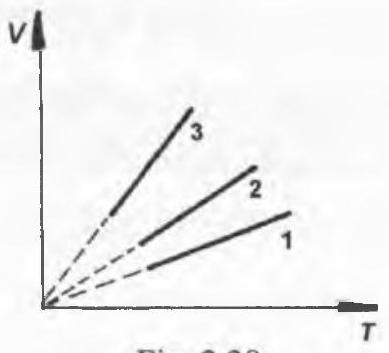
\includegraphics[max width=\textwidth, center]{2025_07_01_5b3ff9fa0d508c8e9f17g-130} Fig. 2.38\\

2.252. Două corpuri au următoarele caracteristici: corpul $1-m_{1}, c_{1}, t_{1}$, iar corpul 2- $m_{2}=m_{1} / 2, c_{2}=4 c_{1}, t_{2}=2 t_{1}$ şi sunt introduse într-un calorimetru de capacitate calorică neglijabilă. Până în momentul realizării echilibrului termic calorimetrul cedează în exterior căldura $Q=\frac{3}{2} m_{1} c_{1} t_{1}$. În această situație, în momentul realizării echilibrului termic temperatura este:\\ A) $(5 / 3) \cdot t_{1}$; B) $t_{1}$; C) $\frac{3}{2} t_{1}$; D) $\frac{7}{6} t_{1}$; E) $1,5 t_{1}$; F) $8 t_{1}$.\\ (Mihai Stafe)\\

2.253. Un gaz ideal cu volumul $V_{1}=0,1 \mathrm{~m}^{3}$, aflat la presiunea $p_{1}=10^{5} \mathrm{~N} / \mathrm{m}^{2}$ parcurge transformarea $p=\alpha V$, unde $\alpha$ este o constantă pozitivă. Lucrul mecanic efectuat de gaz în destinderea sa până la un volum de $n=3$ ori mai mare are valoarea:\\ A) $45 \mathrm{~kJ}$; B) $40 \mathrm{~kJ}$; C) $80 \mathrm{~kJ}$; D) $90 \mathrm{~kJ}$; E) $50 \mathrm{~kJ}$; F) $42 \mathrm{~J}$.\\ (Mihai Stafe)\\

2.254. Un motor termic parcurge ciclul reprezentat în Fig. 2.39 in care $T_{B}=e T_{A}$, unde $e=2,718$. Randamentul ciclului are valoarea:\\ А) 0,25; B) 0,42; C) 0,5; D) 0,99; Е) 0,80; F) 0,20.\\ (Mihai Stafe)\\ 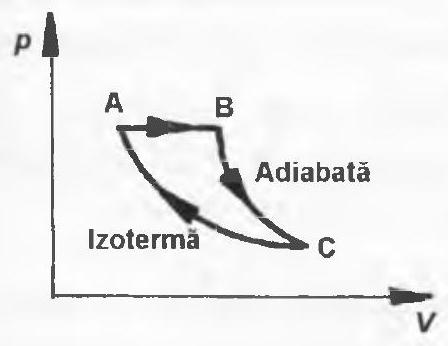
\includegraphics[max width=\textwidth, center]{2025_07_01_5b3ff9fa0d508c8e9f17g-131(1)} Fig. 2.39\\

% Sa speram ca literele din variantele de raspuns nu ne fac probleme
2.255. Un gaz ideal parcurge transformarea ciclică în coordonate ( $p-T$ ) reprezentată în Fig. 2.40. Valoarea maximă a volumului gazului corespunde stării:\\ A) A; B) B; C) C; D) D; E) A+B; F) A+D.\\ (Mihai Stafe)\\ 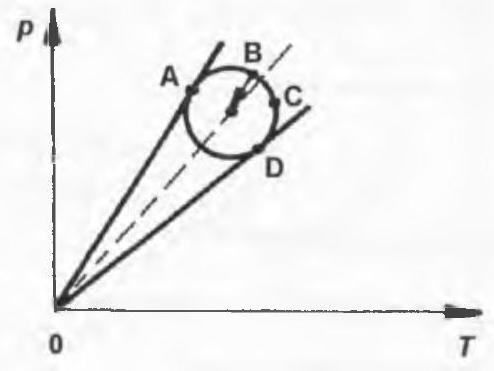
\includegraphics[max width=\textwidth, center]{2025_07_01_5b3ff9fa0d508c8e9f17g-131} Fig. 2.40\\

2.256. Un gaz ideal monoatomic este comprimat după legea $p=\alpha V+\beta$ de la $V_{1}=20$ litri la $V_{2}=1$ litru $\left(\alpha=10^{6} \mathrm{~N} / \mathrm{m}^{5}, \beta=10^{5} \mathrm{~N} / \mathrm{m}^{2}\right)$. Căldura molară a gazului în acest proces este egalǎ cu $\left(C_{V}=\frac{3}{2} R\right)$ :\\ A) $C_{V}$; B) $2 C_{V}$; C) $1,6 C_{V}$; D) $2,3 C_{V}$; E) $2,66 C_{V}$; F) $0,5 C_{V}$.\\ (Mihai Stafe)\\

2.257. Temperatura unui amestec format din $m_{1}=5 \mathrm{~kg}$ apă la temperatura $t_{1}=5^{\circ} \mathrm{C}$ şi $m_{2}=15 \mathrm{~kg}$ apă la temperatura $t_{2}=15^{\circ} \mathrm{C}$ este egală cu:\\ A) $-2^{\circ} \mathrm{C}$; B) $-1^{\circ} \mathrm{C}$; C) $12,5^{\circ} \mathrm{C}$; D) $1^{\circ} \mathrm{C}$; E) $2^{\circ} \mathrm{C}$; F) $5^{\circ} \mathrm{C}$.\\ (Gabriela Cone)\\

2.258. Un gaz ideal cu cu volumul $V_{1}=0,3 \mathrm{~m}^{3}$, aflat la presiunea $p_{1}=3 \cdot 10^{4} \mathrm{~N} / \mathrm{m}^{2}$, parcurge transformarea $p=a V$, unde $a$ este o constantă pozitivă. Lucrul mecanic efectuat de gaz în destinderea sa până la un volum de $n=3$ ori mai mare are valoarea :\\ A) $20 \mathrm{~kJ}$; B) $25 \mathrm{~kJ}$; C) $30 \mathrm{~kJ}$; D) $36 \mathrm{~kJ}$; E) $41 \mathrm{~kJ}$; F) $40 \mathrm{~kJ}$.\\ (Gabriela Cone)\\

2.259. Două vase având volumele $V_{1}$ şi $V_{2}=n V_{1}(n=3)$ conțin gaz ideal la presiunea $p$ şi sunt legate printr-un tub de volum neglijabil. Inițial cele două vase se află la aceeaşi temperatură $T$. Ulterior se încălzeşte vasul $V_{1}$ până la temperatura $T_{1}=k T(k=2)$. Raportul dintre presiunea gazului în stările finală şi inițială este:\\ A) $1 / 3$; B) $1 / 2$; C) $5 / 3$; D) $5 / 6$; E) $8 / 7$; F) $3 / 2$.\\ (Gabriela Cone)\\

2.260. O cantitate de gaz perfect parcurge ciclul din Fig. 2.41 cu randamentul $\eta=2 / 11$. Transformările $1 \rightarrow 2$ şi $3 \rightarrow 4$ sunt izoterme $\left(p_{1}=10^{5} \mathrm{~N} / \mathrm{m}^{2}, \quad p_{2}=2,718 \cdot 10^{5} \quad \mathrm{~N} / \mathrm{m}^{2}\right.$, $T_{1}=T_{2}$ şi $T_{3}=T_{4}=2 T_{1}$ ). Exponentul adiabatic al gazului are valoarea:\\ A) $5 / 3$; B) $7 / 5$; C) $4 / 3$; D) $8 / 7$; E) $10 / 7$; F) 2.\\ (Gabriela Cone)\\ 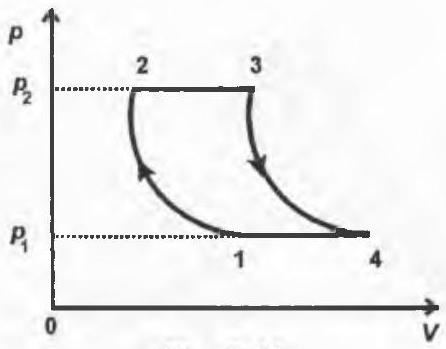
\includegraphics[max width=\textwidth, center]{2025_07_01_5b3ff9fa0d508c8e9f17g-132} Fig. 2.41\\

2.261. Într-un vas închis se află un amestec de oxigen cu azot la temperatura $t=527^{\circ} \mathrm{C}$ şi presiunea $p=10^{5} \mathrm{~N} / \mathrm{m}^{2}\left(\mu_{\mathrm{O}_{2}}=32 \mathrm{~kg} / \mathrm{kmol}, \mu_{\mathrm{N}_{2}}=28 \mathrm{~kg} / \mathrm{kmol}\right)$ in număr egal de moli. Raportul vitezelor pătratice medii ale moleculelor celor două gaze este egal cu:\\ A) $\frac{1}{2}$; B) $\sqrt{\frac{3}{5}}$; C) $\frac{1}{3}$; D) $\sqrt{\frac{7}{8}}$; E) $\sqrt{\frac{5}{7}}$; F) $\frac{2}{3}$.\\ (Gabriela Cone)\\

2.262. Într-un corp de pompă cu volumul $V=5$ litri se află $m=0,8 \mathrm{~kg}$ oxigen ( $\mu_{\mathrm{O}_{2}}=32 \mathrm{~kg} / \mathrm{kmol}$ ) la temperatura $T=320 \mathrm{~K}$. Volumul gazului se reduce izoterm până la valoarea $V_{1}=4 \mathrm{~litri}$. Variația densității oxigenului este:\\ A) $10 \mathrm{~kg} / \mathrm{m}^{3}$; B) $15 \mathrm{~kg} / \mathrm{m}^{3}$; C) $20 \mathrm{~kg} / \mathrm{m}^{3}$; D) $30 \mathrm{~kg} / \mathrm{m}^{3}$; E) $40 \mathrm{~kg} / \mathrm{m}^{3}$; F) $55 \mathrm{~kg} / \mathrm{m}^{3}$.\\ (Gabriela Cone)\\

2.263. Un mol de gaz ideal care parcurge un ciclu Carnot produce lucrul mecanic $L=1,2 \cdot 10^{5} \mathrm{~J}$ în decursul unui ciclu. Temperatura sursei reci este $T_{2}=280 \mathrm{~K}$ şi valoarea minimă atinsă de volumul gazului în decursul ciclului este $V_{m}=0,014 \mathrm{~m}^{3}$. În aceeaşi stare presiunea gazului are valoarea $p_{1}=4,155 \cdot 10^{5} \mathrm{~N} / \mathrm{m}^{2}$. Căldura cedată sursei reci în fiecare ciclu este egală cu:\\ A) $10 \mathrm{~kJ}$; B) $20 \mathrm{~kJ}$; C) $40 \mathrm{~kJ}$; D) $60 \mathrm{~kJ}$; E) $80 \mathrm{~kJ}$; F) $95 \mathrm{~kJ}$.\\ (Gabriela Cone)\\

2.264. Un colector solar constă dintr-o placă plată care absoarbe căldură de la Soare. Printr-un tub ataşat pe spatele plăcii circulǎ apă, care astfel se încălzeşte. Presupunând că acest colector solar de arie de $4 \mathrm{~m}^{2}$ şi puterea primită de la Soare pe unitatea de suprafață este $10^{3} \mathrm{~W} / \mathrm{m}^{2}$, cu ce debit volumic trebuie să curgă apa prin tub pentru ca temperatura să-i crească cu $40^{\circ} \mathrm{C}$ la trecerea prin colector? Se presupune că energia solară cade perpendicular pe colector. (Se dau: $c_{a}=4180 \mathrm{~J} / \mathrm{kg} \cdot \mathrm{K}, \rho_{\mathrm{a}}=10^{3} \mathrm{~kg} / \mathrm{m}^{3}$ ).\\ A) $0,024 \ell / \mathrm{min}$; B) $24 \ell / \mathrm{min}$; C) $14 \ell / \mathrm{min}$; D) $4,18 \ell / \mathrm{min}$; E) $1,4 \ell / \mathrm{min}$; F) $24 \ell / \mathrm{s}$.\\ (Alexandrina Nenciu)\\

2.265. Un clopot pentru scufundări este un cilindru închis la partea superioară şi deschis la partea inferioară. Când este introdus în apă, aerul care se afla inițial în cilindru, rămâne în interior. Dacă cilindrul are înălțimea de $2 \mathrm{~m}$ şi diametrul de $1,5 \mathrm{~m}$ şi este scufundat la o adâncime de $15 \mathrm{~m}$ (Fig. 2.42), până la ce înălțime urcă apa în cilindru?\\ A) $0 \mathrm{~m}$; B) $2 \mathrm{~m}$; C) $1,01 \mathrm{~m}$; D) $1,78 \mathrm{~m}$; E) $1,18 \mathrm{~m}$; F) $0,69 \mathrm{~m}$.\\ (Alexandrina Nenciu)\\ 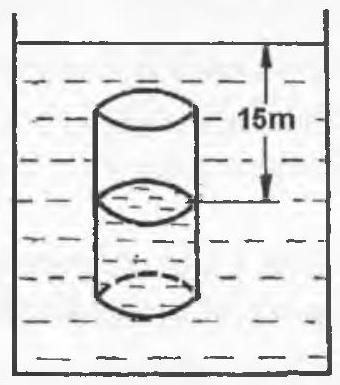
\includegraphics[max width=\textwidth, center]{2025_07_01_5b3ff9fa0d508c8e9f17g-133} Fig. 2.42\\

2.266. Aerul atmosferic conține $75,54 \%$ azot, $23,1 \%$ oxigen și $1,3 \%$ argon, în procente masice. Cu aceste date și cunoscând masele moleculare ale azotului, oxigenului şi argonului, obțineți masa molară medie a aerului. $\left(\mu_{\mathrm{N}_{2}}=28 \mathrm{~g} / \mathrm{mol}\right.$, $\left.\mu_{\mathrm{O}_{2}}=32 \mathrm{~g} / \mathrm{mol}, \mu_{\mathrm{Ar}}=40 \mathrm{~g} / \mathrm{mol}\right)$.\\ A) $32 \mathrm{~g} / \mathrm{mol}$; B) $40 \mathrm{~g} / \mathrm{mol}$; C) $50 \mathrm{~g} / \mathrm{mol}$; D) $1 \mathrm{~g} / \mathrm{mol}$; E) $13 \mathrm{~g} / \mathrm{mol}$; F) $29 \mathrm{~g} / \mathrm{mol}$.\\ (Alexandrina Nenciu)\\

2.267. Un cilindru este împărțit cu un perete în două compartimente egale. Unul din compartimente conține heliu la temperatura de $250 \mathrm{~K}$; celălalt conține oxigen la temperatura de $310 \mathrm{~K}$. Gazele sunt la aceeaşi presiune. Se îndepărtează peretele despărțitor şi gazele se amestecă. Care este temperatura finală ?\\ A) $275 \mathrm{~K}$; B) $300 \mathrm{~K}$; C) $240 \mathrm{~K}$; D) $284 \mathrm{~K}$; E) $232 \mathrm{~K}$; F) $310 \mathrm{~K}$.\\ (Alexandrina Nenciu)\\

2.268. Un calorimetru de cupru, cu masa de $300 \mathrm{~g}$, conține $500 \mathrm{~g}$ apă la temperatura de $15^{\circ} \mathrm{C}$. Un bloc de cupru cu masa de $560 \mathrm{~g}$ aflat la temperatura de $100^{\circ} \mathrm{C}$ este introdus în calorimetru şi se observă că temperatura creşte la $22,5^{\circ} \mathrm{C}$. Neglijând schimbul de căldură cu exteriorul, să se calculeze căldura specifică a cuprului. Căldura specifică a apei este de $4186 \mathrm{~J} / \mathrm{kg} \cdot \mathrm{grad}$.\\ A) $756 \mathrm{~J} / \mathrm{kg} \cdot \mathrm{grad}$; B) $1 \mathrm{kcal} / \mathrm{kg} \cdot \mathrm{grad}$; C) $381 \mathrm{~J} / \mathrm{kg} \cdot \mathrm{grad}$; D) $5 \mathrm{~kJ} / \mathrm{kg} \cdot \mathrm{grad}$; E) $0,2 \mathrm{~J} / \mathrm{g} \cdot \mathrm{grad}$; F) $2 \mathrm{cal} / \mathrm{g} \cdot \mathrm{grad}$.\\ (Ionuț Puică)\\

2.269. Un motor Carnot a cărui sursă caldă are temperatura de $400 \mathrm{~K}$, absoarbe la această temperatură o căldură de $400 \mathrm{~J}$ în fiecare ciclu, şi cedează $320 \mathrm{~J}$ sursei aflate la temperatura scăzută. Care este temperatura acestei surse şi care este randamentul termic al ciclului?\\ A) $0^{\circ} \mathrm{C}$ şi $50 \%$; B) $350 \mathrm{~K}$ şi $18 \%$; C) $47^{\circ} \mathrm{C}$ şi $15 \%$; D) $27^{\circ} \mathrm{C}$ şi $20 \%$; E) $300 \mathrm{~K}$ şi $25 \%$; F) $320 \mathrm{~K}$ şi $20 \%$.\\ (Ionuț Puică)\\

2.270. La ce temperatură viteza pătratică medie (viteza termică) a moleculelor de oxigen este egală cu viteza pătratică medie a moleculelor de hidrogen la $0^{\circ} \mathrm{C}$ ?\\ A) $0^{\circ} \mathrm{C}$; B) $300 \mathrm{~K}$; C) $500 \mathrm{~K}$; D) $100^{\circ} \mathrm{C}$; E) $1911^{\circ} \mathrm{C}$; F) $4097^{\circ} \mathrm{C}$.\\ (Ionuț Puică)\\

2.271. Care este expresia cantitativă a primului principiu al termodinamicii ?\\ A) $U_{1}=U_{2}$; B) $Q+L=$ constant; C) $\Delta U=$ constant; D) $\Delta U=Q-L$; E) $\Delta U=Q+L$; F) $Q=L+U$.\\ (Ionuț Puică)\\

2.272. Care relație este valabilă, conform principiului al II-lea al termodinamicii, în cazul unui proces ciclic ireversibil monoterm ?\\ A) $Q=L>0$; в) $Q>0$; C) $Q>L>0$; D) $Q<L<0$; E) $Q=L<0$; F) $Q=L=0$.\\ (Ionuț Puică)\\

2.273. Care este expresia lucrului mecanic efectuat de un gaz ideal într-o transformare reversibilă izotermă, în care presiunea variază de la $p_{1}$ la $p_{2}$ ?\\ A) $\nu R T \ln \left(p_{2} / p_{1}\right)$; B) $\nu R \ln \left(p_{1} / p_{2}\right)$; C) $\nu C_{V} T$; D) $\nu R T \ln \left(p_{1} / p_{2}\right)$; E) $p_{2} V_{2}-p_{1} V_{1}$; F) $T\left(p_{2}-p_{1}\right)$.\\ (Ionuț Puică)\\

2.274. Să se calculeze randamentul unei maşini termice care funcționează đupả ciclul Stirling compus din izotermele $T_{1}$ şi $T_{2}\left(T_{1}<T_{2}\right)$ şi izocorele $V_{1}$ şi $V_{2}\left(V_{1}<V_{2}\right)$.\\ A) $\eta=R\left(T_{2}-T_{1}\right) \ln V_{2} / V_{1}$; B) $\eta=1-T_{1} / T_{2}$; C) $\eta=\frac{R\left(T_{2}-T_{1}\right) \ln V_{2} / V_{1}}{C_{V}\left(T_{2}-T_{1}\right)-R T_{2} \ln V_{2} / V_{1}}$; D) $\eta=\frac{R\left(T_{2}-T_{1}\right) \ln V_{2} / V_{1}}{C_{V}\left(T_{2}-T_{1}\right)+R T_{2} \ln V_{2} / V_{1}}$; E) $\eta=\frac{R\left(T_{2}-T_{1}\right) \ln V_{1} / V_{2}}{C_{V}\left(T_{2}-T_{1}\right)+R T_{2} \ln V_{2} / V_{1}}$; F) $\eta=\frac{R\left(T_{2}-T_{1}\right) \ln V_{1} / V_{2}}{C_{V}\left(T_{2}-T_{1}\right)-R \ln V_{2} / V_{1}}$.\\ (Mădălina Puică)\\

2.275. Două vase de volume $V_{1}$ şi $V_{2}$, izolate adiabatic, conțin mase egale din acelaşi gaz la temperaturi diferite $T_{1}$ şi $T_{2}$ şi aceeaşi presiune $p$. Vasele sunt unite printr-un tub cu robinet. Să se determine temperatura şi presiunea finală ale sistemului după deschiderea robinetului de comunicare şi stabilirea echilibrului termic.\\ A) $T_{\mathrm{fin}}=\frac{T_{1}+T_{2}}{2}, p_{\mathrm{fin}}=p$; B) $T_{\text {fin }}=T_{1}+T_{2}, p_{\text {fin }}=p$; C) $T_{\text {fin }}=\frac{T_{1}+T_{2}}{2}, p_{\text {fin }}=2 p$; D) $T_{\text {fin }}=\frac{T_{1}-T_{2}}{2}, p_{\text {fin }}=p$; E) $T_{\mathrm{fin}}=2\left(T_{1}+T_{2}\right), p_{\mathrm{fin}}=2 p$; F) $T_{\text {fin }}=\frac{T_{1}+T_{2}}{2}, p_{\text {fin }}=\frac{p}{2}$.\\ (Mădălina Puică)\\

2.276. Un cilindru contine un volum $V_{1}=10$ litri de aer la presiunea $p_{1}=3 \mathrm{~atm}$ şi temperatura $T_{1}=300 \mathrm{~K}$. Care este noul volum şi noua temperatură a gazului dacă: a) presiunea se dublează lent; b) presiunea se dublează brusc. Se cunoaşte exponentul adiabatic al aerului $\gamma=1,4$.\\ A) a) $V_{2}=1 \ell , T_{2}=300 \mathrm{~K}$, b) $V_{2}=5 l , T_{2}=366 \mathrm{~K}$; B) a) $V_{2}=10 \ell , T_{2}=400 \mathrm{~K}$, b) $V_{2}=12 \ell , T_{2}=720 \mathrm{~K}$; C) a) $V_{2}=20 \ell , T_{2}=300 \mathrm{~K}$, b) $V_{2}=7 \ell , T_{2}=420 \mathrm{~K}$; D) a) $V_{2}=5 \ell , T_{2}=300 \mathrm{~K}$, b) $V_{2}=6,1 \ell , T_{2}=366 \mathrm{~K}$; E) a) $V_{2}=5 \ell , T_{2}=300 \mathrm{~K}$, b) $V_{2}=1 \ell , T_{2}=300 \mathrm{~K}$; F) a) $V_{2}=1 \ell , T_{2}=300 \mathrm{~K}$, b) $V_{2}=6,1 \ell , T_{2}=366 \mathrm{~K}$.\\ (Mădălina Puică)\\

2.277. Într-un cilindru închis la ambele capete atârnă un piston agățat de un resort, poziția de echilibru a resortului fiind la partea inferioară a cilindrului. În spațiul de sub piston se introduce o cantitate de gaz astfel încât pistonul să se ridice la înălțimea $h$. La ce înalțime $h_{1}$ se va stabili pistonul când temperatura gazului va creşte de la $T$ la $T_{1}$ ?\\ A) $h_{1}=\frac{h}{2}$; B) $h_{1}=h \sqrt{\frac{T}{T_{1}}}$; C) $h_{\mathrm{I}}=h \sqrt{\frac{T_{1}}{T}}$; D) $h_{1}=h \frac{T_{1}}{T}$; E) $h_{1}=2 h \sqrt{\frac{T}{T_{1}}}$; F) $h_{1}=2 h$.\\ (Mădălina Puică)\\

2.278. Cu câte grade se va modifica temperatura unui glonț când intră într-o scândură cu viteza de $400 \mathrm{~m} / \mathrm{s}$ şi iese cu viteza $300 \mathrm{~m} / \mathrm{s}$ ? Se dă: $c=125,4 \mathrm{~J} / \mathrm{kg} \cdot \mathrm{grad}$.\\ A) $\Delta T=2 \mathrm{~K}$; B) $\Delta T=20 \mathrm{~K}$; C) $\Delta T=2^{\circ} \mathrm{C}$; D) $\Delta T=20^{\circ} \mathrm{C}$; E) $\Delta T=280 \mathrm{~K}$; F) $\Delta T=28^{\circ} \mathrm{C}$.\\ (Radu Chişleag)\\

2.279. Masa molară medie a unui amestec de molecule de azot şi de oxigen dintr-o butelie pentru scafandri este $\mu=30 \mathrm{~g} \cdot \mathrm{~mol}^{-1}$. Dacă în amestec sunt $0,014 \mathrm{~kg}$ de azot, care este masa oxigenului din butelie ?\\ A) $16 \mathrm{~g}$; B) $160 \mathrm{~g}$; C) $160 \mathrm{~g} \cdot \mathrm{~mol}^{-1}$; D) $32 \mathrm{~g}$; E) $123 \mathrm{~g}$; F) $9,1 \mathrm{~g}$.\\ (Radu Chişleag)\\

2.280. Care este presiunea gazului dintr-o incintă în care se află $7,2 \mathrm{~kg}$ acetilenă $\left(\mathrm{C}_{2} \mathrm{H}_{2}\right)$ cu densitatea de $18 \mathrm{mg} / \mathrm{cm}^{3}$ şi viteza termică a moleculelor de $500 \mathrm{~ms}^{-1}$ ?\\ A) $1 \mathrm{~at}$; B) $1 \mathrm{~atm}$; C) $1,5 \cdot 10^{5} \mathrm{~N} / \mathrm{m}^{2}$; D) $1,5 \mathrm{MN} \cdot \mathrm{m}^{-2}$; E) $15 \cdot 10^{5} \mathrm{~N} \cdot \mathrm{~m}^{-1}$; F) $15 \mathrm{~N} \cdot \mathrm{~cm}^{-2}$.\\ (Radu Chişleag)\\

2.281. O sticlă de şampanie a fost etanşată la temperatura de $27^{\circ} \mathrm{C}$, la presiune normală, cu un dop care astupă gâtul cilindric al sticlei ce are secțiunea de $3 \mathrm{~cm}^{2}$. Până la ce temperatură poate fî încălzită sticla, înaintea începerii fermentării fără ca dopul să sară, dacă pentru introducerea lui a fost necesar un efort de $5 \mathrm{~N}$ şi se neglijează variația coeficientului de frecare cu temperatura şi procesele de dilatare.\\ A) $127^{\circ} \mathrm{C}$; B) $-73^{\circ} \mathrm{C}$; C) $350^{\circ} \mathrm{C}$; D) $350 \mathrm{~K}$; E) $250 \mathrm{~K}$; F) $412,5 \mathrm{~K}$.\\ (Radu Chişleag)\\

2.282. O maşină termică ideală funcționează cu $1,5 \mathrm{kmol}$ de azot, după un ciclu Carnot reversibil. Ştiind că temperatura minimă este $27^{\circ} \mathrm{C}$ şi maşina furnizează $60 \mathrm{~kJ}$ la fiecare ciclu parcurs, să se determine numărul de molecule de azot la temperatura maximă. Se cunoaşte: $N_{A}=6 \cdot 10^{23} \mathrm{~mol}^{-1}$.\\ A) $9 \cdot 10^{26} \mathrm{~mol} \cdot \mathrm{dm}^{-3}$; B) $4 \cdot 10^{26}$; C) $9 \cdot 10^{26}$ molecule; D) $4 \cdot 10^{23}$; E) $6,023 \cdot 10^{26}$; F) $9 \cdot 10^{25}$.\\ (Radu Chişleag)\\

2.283.* O oală de fiert la presiune constantă, în care se găsesc $5 \mathrm{~litri}$ de apă, este încălzită pe un reşou ce consumă $12 \mathrm{~g}$ de benzină pe minut şi are un randament de încǎlzire de 0,66. Care va fì viteza de creştere a masei apei din vas prin fierbere după stabilizarea temperaturii vasului? ( $q_{B}=50 \mathrm{MJ} / \mathrm{kg} ; \lambda_{v}=2,2 \mathrm{MJ} / \mathrm{kg}$ ).\\ А) $6,75 \mathrm{~g} / \mathrm{s}$; B) $-3 \mathrm{~g} / \mathrm{s}$; C) $2 \mathrm{~g} / \mathrm{s}$; D) $-3 \mathrm{~kg}$; E) $2 \mathrm{~kg}$; F) $-5 \mathrm{~litri} / \mathrm{h}$.\\ (Radu Chişleag)\\

2.284. O masă $m=10 \mathrm{~g}$ de hidrogen ( $\mu=2 \mathrm{~kg} / \mathrm{kmol}$ )se află la presiunea $p=5 \cdot 10^{5} \mathrm{~N} / \mathrm{m}^{2}$ şi temperatura $t_{1}=17^{\circ} \mathrm{C}$. Dupã încălzirea izobară, gazul ocupă volumul $V_{2}=25 \mathrm{dm}^{3}$. Să se determine variația energiei interne dacă se cunoaşte căldura molară izobară $C_{p}=\frac{7}{2} R$.\\ A) $1 \mathrm{~kJ}$; B) $10000 \mathrm{~J}$; C) $500 \mathrm{~J}$; D) 0; E) $1126,25 \mathrm{~J}$; F) $550 \mathrm{~J}$.\\ (Ion Gurgu)\\

2.285. Într-un vas de volum $V=0,1 \mathrm{~m}^{3}$ se găseşte aer la presiunea $p_{1}=5 \cdot 10^{5} \mathrm{~N} / \mathrm{m}^{2}$. Aerul este răcit izocor şi cedează căldura $Q=50 \mathrm{~kJ}$. Să se afle presiunea finală a gazului cunoscând căldura molară izocoră a aerului $C_{V}=\frac{5}{2} R$, unde $R$ este constanta universală a gazelor ideale.\\ A) $10^{5} \mathrm{~N} / \mathrm{m}^{2}$; B) $3 \cdot 10^{5} \mathrm{~N} / \mathrm{m}^{2}$; C) $100 \mathrm{~kPa}$; D) $2 \cdot 10^{5} \mathrm{~N} / \mathrm{m}^{2}$; Е) 0; F) $1000 \mathrm{~N} / \mathrm{m}^{2}$.\\ (Ion Gurgu)\\

2.286. Un motor ideal, care funcționează după un ciclu Carnot, absoarbe căldura $Q_{1}=3000 \mathrm{~J}$ de la o sursă caldă aflată la temperatura $T_{1}=600 \mathrm{~K}$. Dacă temperatura sursei reci este $T_{2}=300 \mathrm{~K}$, să se determine căldura $Q_{2}$ cedată sursei reci.\\ A) $1000 \mathrm{~J}$; B) $1,5 \mathrm{~kJ}$; C) $1 \mathrm{~kJ}$; D) $3000 \mathrm{~J}$; E) 0; F) $600 \mathrm{~J}$.\\ (Ion Gurgu)\\

2.287. Un balon ce contine o cantitate de azot la temperatura $t=17^{\circ} \mathrm{C}$ se mişcã cu viteza $v=100 \mathrm{~m} / \mathrm{s}$. Care va fi temperatura gazului dacă balonul se opreşte brusc? (Se neglijează pierderile de căldură prin pereți).\\ A) $10^{\circ} \mathrm{C}$; B) $283 \mathrm{~K}$; C) $24^{\circ} \mathrm{C}$; D) $-24^{\circ} \mathrm{C}$; E) $249 \mathrm{~K}$; F) $0^{\circ} \mathrm{C}$.\\ (Ion Gurgu)\\

2.288. Un balon cu hidrogen cu volumul $V=10 \mathrm{dm}^{3}$ aflat la temperatura $t=7^{\circ} \mathrm{C}$ are presiunea de $4,9 \cdot 10^{6} \mathrm{~N} / \mathrm{m}^{2}$. Ce cantitate de gaz trebuie scoasă din balon astfel încât la $17^{\circ} \mathrm{C}$ să aibă aceeași presiune?\\ A) $1,45 \cdot 10^{-6} \mathrm{~kg}$; B) $1,45 \cdot 10^{-3} \mathrm{~kg}$; C) $1,45 \cdot 10^{-3} \mathrm{~g}$; D) $1,2 \mathrm{~moli}$; E) $0,725 \mathrm{moli}$; F) $0,725 \mathrm{kmol}$.\\ (Ion Gurgu)\\

2.289. Printr-o conductă de sectiune $S=5 \mathrm{~cm}^{2}$ se scurge heliu la presiunea $p=3,9 \cdot 10^{5} \mathrm{~N} / \mathrm{m}^{2}$ şi temperatura $t=17^{\circ} \mathrm{C}$. Cu ce viteză se scurge gazul dacă în timpul $t=10 \mathrm{~min}$ s-au scurs $m=2 \mathrm{~kg}$ de gaz.\\ A) $10,3 \mathrm{~m} / \mathrm{s}$; B) $40 \mathrm{~m} / \mathrm{s}$; C) $9,9 \mathrm{~km} / \mathrm{s}$; D) $9,81 \mathrm{~m} / \mathrm{s}^{2}$; E) $1,1 \mathrm{~m} / \mathrm{s}$; F) $0 \mathrm{~m} / \mathrm{s}$.\\ (Mihai Piscureanu)\\

2.290. Să se calculeze randamentul ciclului din Fig. 2.43. Se cunoaşte $\gamma=5 / 3$.\\ A) $\eta=10 \%$; B) $\eta=9 \%$; C) $\eta=7 \%$; D) $\eta=5,5 \%$; E) $\eta=8 \%$; F) $\eta=5 \%$.\\ (Mihai Piscureanu)\\ 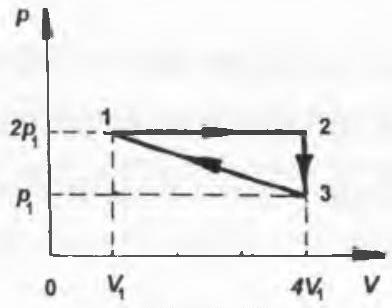
\includegraphics[max width=\textwidth, center]{2025_07_01_5b3ff9fa0d508c8e9f17g-138} Fig. 2.43\\

2.291. O cantitate de $\nu$ kmoli de gaz ideal diatomic, aflat la presiunea $p_{1}$ şi temperatura $T_{1}$, se destinde după legea $T=a V-b V^{2}$, unde $a$ şi $b$ sunt douā constante. Să se determine variația energiei interne a gazului atunci când volumul lui se măreşte de $n$ ori.\\ A) $\Delta U=\frac{5 \nu R V_{1}}{2}(n-1)\left[a-b V_{1}(n+1)\right]$; B) $\Delta U=5 \nu R V_{1}(n-1)\left[a-b V_{1}(n+1)\right]$; C) $\Delta U=\frac{5 R V_{1}}{2 \nu}(n-1)\left[a-b V_{1}(n+1)\right]$; D) $\Delta U=\frac{5 \nu R V_{1}}{2}(n-1)\left[a-\frac{b V_{1}}{n+1}\right]$; E) $\Delta U=\frac{5 \nu R V_{1}}{2}(n-1) \frac{a-b V_{1}}{n+1}$; F) $\Delta U=\frac{5 \nu R V_{1}}{2}(n-1)\left(a-b V_{1}\right)(n+1)$.\\ (Mihai Piscureanu)\\

2.292. Un kilomol de gaz ideal se destinde de la volumul $V_{1}$ la volumul $V_{2}=5 V_{1}$ după legea $T=a V+b V^{2}$, unde $a$ şi $b$ sunt constante. Să se determine lucrul mecanic efectuat de gaz.\\ A) $4 R V_{1}\left(a-4 b V_{1}\right)$; B) $3 R V_{1}\left(a-4 b V_{1}\right)$; C) $4 R V_{1}\left(a-3 b V_{1}\right)$; D) $-5 R V_{1}\left(a+4 b V_{1}\right)$ E) $-4 R V_{1}\left(a+3 b V_{1}\right)$; F) $-3 R V_{1}\left(a-4 b V_{1}\right)$.\\ (Mihai Piscureanu)\\

2.293. Căldura specifică la volum constant a unui gaz este $c_{V}$, iar densitatea sa în condiții normale $\left(p_{0}, T_{0}\right)$ este $\rho_{0}$. Exponentul adiabatic $\gamma$ va fi:\\ A) $\gamma=1+\frac{p_{0}}{c_{V} \mathrm{P}_{0} T_{0}}$; B) $\gamma=\frac{p_{0}}{c_{V} \rho_{0} T_{0}}$; C) $\gamma=1-\frac{p_{0}}{c_{V} \rho_{0} T_{0}}$; D) $\gamma=\frac{c_{V} \rho_{0} T_{0}}{\rho_{0}}$; E) $\gamma=1+\frac{c_{V} \rho_{0} T_{0}}{\rho_{0}}$; F) $\gamma=1-\frac{c_{V} \rho_{0} T_{0}}{\rho_{0}}$.\\ (Rodica Bena)\\

2.294.* Presiunea unui gaz ideal creşte de 2 ori prin încălzire izocoră. Atunci viteza termică a moleculelor gazului:\\ A) creşte de 2 ori; B) scade de 2 ori; C) creşte de 4 ori; D) scade de 4 ori; E) creşte de $\sqrt{2}$ ori; F) scade de $\sqrt{2}$ ori.\\ (Rodica Bena)\\

2.295. În coordonate $(p, \rho)$ o transformare se reprezintă ca în Fig. 2.44. Transformarea este:\\ A) izocoră; B) izotermă; C) adiabată; D) descrisă de ecuația $p=a V(a=c t)$; E) generală; F) izobară.\\ (Rodica Bena)\\ 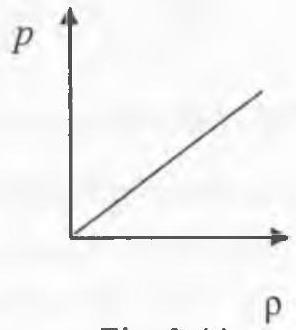
\includegraphics[max width=\textwidth, center]{2025_07_01_5b3ff9fa0d508c8e9f17g-139} Fig. 2.44\\

2.296. Într-un vas se află un amestec de $He$ şi $\mathrm{H}_{2}$ la presiunea $p$. Dublând masa heliului din vas, fără a modifica temperatura, presiunea devine $p^{\prime}=1,2 p$. Raportul maselor inițiale de substanță $\frac{m_{\mathrm{He}}}{m_{\mathrm{H}_{2}}} ;\left(\mu_{\mathrm{He}}=4 \mathrm{~kg} / \mathrm{Kmol} ; \mu_{\mathrm{H}_{2}}=2 \mathrm{~kg} / \mathrm{Kmol}\right)$ este:\\ A) 0,25; B) 1; C) 2; D) 0,8; E) 1,2; F) 0,5.\\ (Rodica Bena)\\

2.297. O maşină termică funcționează după un ciclu Carnot având temperaturile celor două izvoare de căldură $T$ şi respectiv $3 T$. Lucrul efectuat de maşină într-un ciclu este $900 \mathrm{~J}$. Lucrul efectuat de gaz în destinderea izotermă va fi:\\ A) $900 \mathrm{~J}$; B) $600 \mathrm{~J}$; C) $1,35 \mathrm{~kJ}$; D) $1,8 \mathrm{~kJ}$; E) $300 \mathrm{~J}$; F) $750 \mathrm{~J}$.\\ (Rodica Bena)\\

2.298. Un motor termic având ca agent de lucru un gaz ideal cu $\gamma=\frac{5}{3}$, funcționează după ciclul $1-2-$ transformare de tipul $p=a V$ ( $a=$ const.) şi $V_{2}=2 V_{1}, 2-3$ - o destindere adiabatică si 3-1 - o comprimare izobară. (Se dă: $2^{8 / 5} \cong 3,03$ ). Randamentul acestui motor este:\\ А) $25 \%$; B) $35 \%$; C) $11,5 \%$; D) $15,4 \%$, Е) $20,4 \%$; F) $30,2 \%$.\\ (Rodica Bena)\\

2.299. Într-un proces izobar un gaz efectuează lucrul mecanic $L=800 \mathrm{~J}$ şi schimbă cu exteriorul căldură $Q=2800 \mathrm{~J}$. Exponentul adiabatic al gazului este:\\ A) $\frac{5}{3}$; B) $\frac{7}{5}$; C) $\frac{3}{2}$; D) $\frac{5}{2}$; E) $\frac{7}{2}$; F) $\frac{4}{3}$.\\ (Rodica Bena)\\

2.300. Un amestec format din $\nu_{1}=3$ moli de gaz monoatomic $\left(\gamma_{1}=\frac{5}{3}\right)$ şi $\nu_{2}=5$ moli de gaz biatomic $\left(\gamma_{2}=\frac{7}{5}\right)$ are exponentul adiabatic:\\ А) 1,53; B) 1,8; C) 1,47; D) $\frac{10}{7}$; E) $\frac{13}{8}$; F) $\frac{11}{8}$.\\ (Rodica Bena)\\

2.301. Un gaz ideal având $\gamma=1,4$ ocupă volumul $V_{1}=4 \mathrm{dm}^{3}$ la presiunea $p_{1}=8 \cdot 10^{5} \mathrm{~Pa}$. În urma unei destinderi adiabatice gazul efectuează lucrul mecanic $L=6 \mathrm{~kJ}$. Raportul temperaturilor stărilor finală şi inițială este:\\ А) 0,4; B) 0,5; C) 2,5; D) 2; E) 1; F) 0,25.\\ (Rodica Bena)\\

2.302. În cursul unui proces termodinamic dependența presiunii unui mol de gaz ideal de volum este dată de relația $p=a V^{-2 / 3}$ ( $a=$ const.). Din starea cu volumul $V$ şi temperatura $T_{1}=300 \mathrm{~K}$ gazul trece în starea cu volumul $8 V$ şi temperatura $T_{2}$, schimbând cu exteriorul căldura. (Se dau: $\gamma=7 / 5 ; R=8,31 \mathrm{~J} / \mathrm{mol} \cdot \mathrm{K}$ )\\ A) $13,7 \mathrm{~kJ}$; B) $27,4 \mathrm{~kJ}$; C) $6,85 \mathrm{~kJ}$; D) $4,57 \mathrm{~kJ}$; E) 0; F) $5,2 \mathrm{~kJ}$.\\ (Rodica Bena)\\

2.303.* Într-un proces adiabatic presiunea unui gaz ideal $(\gamma=5 / 3)$ creşte de 32 de ori. Raportul vitezelor termice ale moleculelor în cele două stări ( $v_{2} / v_{1}$ ) este:\\ А) 4; B) 16; C) 2; D) 8; E) $\sqrt{2}$; F) $1 / 2$.\\ (Rodica Bena)\\

2.304. Unitatea de măsură a presiunii scrisă în funcție de unități ale mărimilor fundamentale din SI este:\\ A) $\mathrm{m}^{-1} \mathrm{~kg} \mathrm{~s}^{-2}$; B) $\mathrm{m}^{-1} \mathrm{gs}^{-2}$; C) $\mathrm{m}^{-2} \mathrm{~kg} \mathrm{~s}^{-1}$; D) $\mathrm{m}^{-1} \mathrm{~kg}^{-1} \mathrm{~s}^{-2}$; E) $\mathrm{m}^{-1} \mathrm{~kg} \mathrm{~s}^{-3}$; F) $\mathrm{m}^{-2} \mathrm{Kg} \mathrm{s}^{-2}$.\\ (Ioana Ivaşcu)\\

2.305. Pentru un gaz se cunoaşte coeficientul adiabatic $\gamma$. Căldura molară și la presiune constantă $C_{p}$ şi căldura molară la volum constant $C_{v}$ au valorile:\\ A) $C_{p}=\frac{R \gamma}{\gamma-1} , C_{v}=\frac{R}{\gamma-1}$; В) $C_{p}=\frac{R}{\gamma-1} , C_{v}=\frac{R \gamma}{\gamma-1}$; C) $C_{p}=\frac{R}{\gamma-1} , C_{v}=\frac{R(\gamma-1)}{\gamma}$; D) $C_{p}=\frac{R(\gamma-1)}{\gamma-R} , C_{v}=\frac{R}{\gamma-R}$; Е) $C_{p}=\frac{R \gamma}{\gamma-2} , C_{v}=\frac{R}{\gamma-2}$; F) $C_{p}=\frac{5 R \gamma}{2(\gamma-1)} , C_{v}=\frac{3 R}{2(\gamma-1)}$.\\ (Ioana Ivaşcu)\\

2.306. O cantitate de gaz biatomic ( $C_{v}=\frac{3 R}{2}$ ) evoluează după legea $V=a T^{-1}$. Căldura molară a gazului în decursul destinderii este:\\ A) $C=\frac{3 R}{2}$; B) $C=\frac{5 R}{2}$; C) $C=\frac{R}{2}$; D) $C=3 R$; E) $C=R$; F) $C=2 R$.\\ (Ioana Ivaşcu)\\

2.307.* Un motor termic funcționează după un ciclu Carnot între temperaturile $t_{1}=27^{\circ} \mathrm{C}$ şi $t_{2}=627^{\circ} \mathrm{C}$. Raportul vitezelor termice extreme atinse în ciclu este :\\ A) $\frac{v_{T_{2}}}{v_{T_{1}}}=\sqrt{2}$; B) $\frac{v_{T_{2}}}{v_{T_{1}}}=2$; C) $\frac{v_{T_{2}}}{v_{T_{1}}}=\sqrt{3}$; D) $\frac{v_{T_{2}}}{v_{T_{1}}}=\sqrt{23,22}$; E) $\frac{v_{T_{2}}}{v_{T_{1}}}=3$; F) $\frac{v_{T_{2}}}{v_{T_{1}}}=2 \sqrt{2}$.\\ (Ioana Ivaşcu)\\

2.308. Un motor termic funcționează după un ciclu Carnot având randamentul $\eta=0.6$. Ştiind că în decursul unui ciclu motorul primeşte căldura $Q_{p}=1200 \mathrm{~J}$ să se calculeze căldura cedată de sistem mediului exterior.\\ A) $Q_{c}=480 \mathrm{~J}$; B) $Q_{c}=680 \mathrm{~J}$; C) $Q_{c}=560 \mathrm{~J}$; D) $Q_{c}=600 \mathrm{~J}$; E) $Q_{c}=400 \mathrm{~J}$; F) $Q_{c}=402 \mathrm{~J}$.\\ (Ioana Ivaşcu)\\

2.309. Într un vas se află $\nu$ moli de gaz ideal având masa molară $\mu$ la presiunea $p$ şi temperatura $T$. Densitatea gazului în aceste condiții este:\\ A) $\rho=\frac{\nu p}{R T}$; B) $\rho=\frac{\mu p}{T}$; C) $\rho=\frac{\mu p}{R T}$; D) $\rho=\frac{R T}{\mu p}$; E) $\rho=\frac{\mu p T}{R}$; F) $\rho=\frac{\mu p R}{T}$.\\ (Ioana Ivaşcu)\\

2.310. O maşină termică având randamentul $\eta=0.3$ cedează căldura $Q_{c}=210 \mathrm{~J}$ în decurs de un ciclu. Puterea utilă a maşinii dacă se efectuează $n=10$ cicluri pe secundă este:\\ A) $P=900 \mathrm{~W}$; B) $P=1000 \mathrm{~W}$; C) $P=450 \mathrm{~W}$; D) $P=600 \mathrm{~W}$; E) $P=300 \mathrm{~W}$; F) $P=630 \mathrm{~W}$.\\ (Ioana Ivaşcu)\\

2.311. O cantitate de gaz ideal ocupă volumul $V_{1}$ la presiunea $p$. Gazul se dilată izobar primind căldura $Q$. Volumul final al gazului este:\\ A) $\frac{Q(\gamma-1)}{p \gamma}+V_{1}$; B) $\frac{Q(\gamma-1)}{p}+V_{1}$; C) $p \frac{Q(\gamma-1)}{\gamma}+V_{1}$; D) $\frac{Q \gamma}{p(\gamma-1)}+V_{1}$; E) $\frac{Q \gamma(\gamma-1)}{p}+V_{1}$; F) $\frac{Q(\gamma-1)}{p(\gamma-2)}+V_{1}$.\\ (Ioana Ivaşcu)\\

2.312. O cantitate de gaz ideal parcurge un ciclu format din două izocore $V_{1}$, $V_{2}=n V_{1}$ şi două izobare $p_{1}, p_{2}=k p_{1}$. Randamentul ciclului are expresia:\\ A) $\eta=\frac{(n-1)(k-1)(\gamma-1)}{(k-1)+\gamma(n-1)}$; В) $\eta=\frac{(k-1)(\gamma-1)}{(k-1)+\gamma(n-1)}$; C) $\eta=\frac{(n-1)(k-1)(\gamma-1)}{(k-1)+\gamma}$; D) $\eta=\frac{(n-1)(k-1)}{(k-1)+\gamma(n-1)}$; E) $\frac{\gamma}{\gamma-1}\left[\frac{1}{(n-1)}+\frac{k n}{k-1}\right]$; F) $\eta=\frac{(n-1)(\gamma-1)}{(k-1)+\gamma(n-1)}$.\\ (Ioana Ivaşcu)\\

2.313. $\nu$ moli de gaz ideal evoluează după legea $T=a p^{3}$ de la starea inițială de temperatură $T_{0}$ la starea finală în care temperatura este $T=k T_{0}$. Lucrul mecanic efectuat de gaz în această transformare este:\\ A) $L=\frac{2 \nu R T_{0}(k-1)}{3}$; B) $L=\frac{3 \nu R T_{0}^{\prime}(k-1)}{2 k}$; C) $L=\frac{\nu R T_{0}(1-k)}{2}$; D) $L=\nu R T_{0}(k-1)^{2}$; E) $L=\nu R T_{0}(k-1)$; F) $L=\nu R T_{0} k(k-1)$.\\ (Ioana Ivaşcu)\\

2.314. O cantitate de $\nu$ moli de gaz ideal se găseşte în starea inițială la temperatura $T_{0}$ şi suferă o transformare izobară efectuând lucrul mecanic $L$. Temperatura gazului în starea finală este:\\ A) $T_{0}+\frac{4 L}{\nu R}$; B) $T_{0}+\frac{L}{2 \nu R}$; C) $T_{0}+\frac{2 L}{\nu R}$; D) $T_{0}+\frac{\nu L}{R}$; E) $T_{0}+\frac{L}{\nu R}$; F) $T_{0}+\frac{2 \nu L}{R}$.\\ (Ioana Ivaşcu)\\

%% End %%